\documentclass[unicode,master,printedition]{seuthesis} % 本科
% \documentclass[master]{seuthesis} % 硕士
% \documentclass[doctor]{seuthesis} % 博士
% \documentclass[engineering]{seuthesis} % 工程硕士
\usepackage{booktabs}
\usepackage{amsmath}
\usepackage{subfig}
\renewcommand\figureautorefname{图}
\renewcommand\tableautorefname{表}
%\usepackage{graphicx}
\DeclareGraphicsExtensions{.jpg,.pdf}
\graphicspath{{fig/}{figure/}{images/}}
%\hypersetup{unicode=false}
 % 这里是导言区

\begin{document}
\categorynumber{000} % 分类采用《中国图书资料分类法》
\UDC{000}            %《国际十进分类法UDC》的类号
\secretlevel{公开}    %学位论文密级分为"公开"、"内部"、"秘密"和"机密"四种
\studentid{082200}   %学号要完整,前面的零不能省略。
\title{驾驶人行为特性对交通流的影响研究}{}{Thesis Title}{subtitle}
\author{吴\quad{}璠}{WU Fan}
\advisor{陆\quad{}建}{教授}{LU Jian}{Prof.}
%\coadvisor{副导师}{副教授}{Co-advisor's Name}{Associate Prof.} % 没有
                                % 可以不填
% \degree{工学硕士} % 详细学位名称
\major[12em]{交通运输规划与管理}
\defenddate{}
\authorizedate{}
%\department{交通学院}{Trasnportation College}
%\duration{2007.11—2008.6}
%\address{河海院2楼}
\maketitle

\begin{abstract}{中文关键字}
  中文摘要。
\end{abstract}

\begin{englishabstract}{English Keywords}
  English abstract.
\end{englishabstract}

%\begin{terminology}
%  本论文专用术语的注释表
%\end{terminology}

\begin{Main} % 开始正文

%\chapter{绪论(前言)}
%\section{研究的主要内容}
%\subsection{...}
%\subsubsection{...}
%\section{需要解决的问题}
%使得论文符合要求\cite{seugs:standard}。
%
%\chapter{...}
%...
\chapter{绪论}
\section{立题的背景和意义}
这是测试\cite{seugs:standard}

车辆的行驶是由驾驶人操纵有关机构实现的,驾驶人不仅是道路交通系统的信息处理者和决策者,也是道路交通系统的调节者和控制者,是道路交通系统中最活跃的要素。车辆的行驶状态是驾驶人所采取的驾驶行为的作用结果,而驾驶行为是在一定的外部环境下,驾驶人生理、心理和操作技能等驾驶特性相互作用的综合体现。不同驾驶人的生理状况和心理素质不同、驾驶操作技能也有差异,因此驾驶行为存在差异。不同驾驶人表现出不同的驾驶行为,同一名驾驶人在不同的外部环境和自身状态下的驾驶行为也不同。驾驶人行为特性具体的外在表现主要包括,在动态交通条件下,驾驶人的反应时间,速度选择,加速度选择,跟驰距离选择,变道决策与间隙接受等一系列特性。

长期以来,我国机动车为各种企事业单位所有,机动车驾驶人均为专业驾驶人,专业驾驶人的驾驶技能熟练程度、驾驶特性等方面的差异都较小。随着大量小汽车进入家庭,产生了大量的非专业驾驶人,非专业驾驶人在生理、心理以及驾驶操作技能等方面与专业驾驶人都存在明显的差异。而在传统的道路交通规划、设计与交通管理的研究和工程设计中,从宏观上假设驾驶人的驾驶特性相似和受同一普遍规律影响,与现今的真实情况存在差异。这种假设没有体现驾驶人操作活动在复杂环境下的不确定性和不一致性,没有反映同一驾驶员在不同环境下驾驶行为特性的差异,没有反映大量驾驶人驾驶特性的微观差异对宏观交通流的影响,没有反映出驾驶人不同的驾驶特性对道路交通流的影响作用关系,这与现今真实的交通状况存在显著的差异。在此基础上进行的道路交通规划、设计与交通管理难以符合真实的交通现象,降低了交通规划、设计方案与交通管理措施的合理性与实施效果,同时也增加了交通事故的潜在危险性。

通过研究驾驶人行为特性对交通流的影响,将有助于对驾驶特性、驾驶行为与道路交通流的影响关系有更加深刻的理解;将有助于从人的因素的角度分析各种复杂交通流现象的形成和演化过程;将有助于确定影响道路交通安全的人的因素,为进一步探究改善交通流状况和提高交通安全性提供有力的理论支持;也可以为智能车辆、驾驶辅助支持系统等设备的研制提供理论支持。总之,研究驾驶人行为特性对道路交通流的影响,对提高道路交通系统运输效率和交通安全性具有重要意义,对我国今后的道路交通规划、设计、管理、控制也有重要的理论和应用价值。



\section{国内外研究概况}

\subsection{驾驶人行为特性研究}

Cheng-Chen Kou(1997)研究了高速公路汇入匝道处驾驶人的跟驰和汇入时的间隙接受行为。研究发现驾驶人匝道处的汇入行为,并不与任何单一的参数如汇入速度、主线流量、跟车间距与时距、速度差等显著相关,而各参数的组合能更好的解释驾驶人的驾驶行为[1]。Dario D. Salvucci 和Andrew Liu(2002)对驾驶人变道过程中的操纵和眼动情况进行了分析[2]。Samer Hani Hamdar(2004)在Gipp’s跟驰模型的基础上融入了紧急条件下驾驶人的不同驾驶类型,并对驾驶人的特性进行了敏感性分析[3]。Letian Yang(2007)通过城市道路、乡村道路和高速公路的实测数据对自由流和非自由条件下的驾驶人的速度选择和加减速行为进行了研究,并对不同行为的驾驶人进行了分类。研究发现对于不同的道路驾驶人的速度行为差异明显,并与交通流条件高度相关;驾驶人一般会选择高于限速值不超过10\%的速度;根据驾驶人群体可分为进攻型、防守型、和一般型三类,进攻型倾向于选择高于限速的车速,防守型相反,一般型选择不超过限速太多的车速;驾驶人的加减速选择在非自由流条件下变化更大;在自由流条件下,驾驶人的加减速依赖于瞬时速度。在中低速情况下,加减速率随速度增加而减小。而在高速条件下较为稳定;不同类型驾驶人的加减速选择差异明显,进攻型驾驶人加减速率较大而防守型相反[4]。Feng Xu(2007)研究了环形交叉口驾驶人的间隙接受行为,研究从视频数据中提取事件信息,用最大似然法和Raff法对临界车头时距和跟车时距进行了估计并进行了比较。研究发现交织流量和环道车速与临界车头时距和跟车时距呈现负相关性[5]。KEVIN PATRICK HEASLIP II(2007)在跟驰模型中加入了驾驶人对车道改变的熟悉程度、适应性、攻击性,研究了施工区域驾驶人的驾驶行为[6]。Dalia Said(2008)根据高速公路不同路段的实测数据,从驾驶人劳动强度的角度分析了驾驶人的加减速和方向盘操作行为,并与高速公路线形设计的安全性进行了关联性分析[7]。Hwasoo Yeo(2008)根据实际轨迹数据研究了驾驶人的微观非对称行为,在驾驶模型中加入了操作差错和驾驶人预期,解释了交通流的滞后、不稳定、通行能力下降、换道松弛和时走时停现象,并分析了基本图中的D型和A型曲线[8]。

孔繁森 (2004) 依据Kuipers的定性仿真方法对熟练驾驶人和刚学会开车的驾驶人,在具有不同曲率半径和路面情况的一段道路上所做出的车速选择做了定性推理,给出了两类不同驾驶人驾车行为的定性状态描绘图和相应的车速曲线变化图[9]。张开冉 (2008) 对新驾驶人的反应时进行测试,与一定样本量的对照组相应指标作比较,结果表明信息复杂度较大时,两组间反应时差异较为显著[10]。王晶 (2008) 基于驾驶人性别对城市快速路跟驰模型进行了研究[11]。范红静 (2008) 研究了真实道路交通环境下专业与非专业驾驶人动态视觉特性的差异,并提出了满足驾驶人行车安全的交叉口通行能力的计算方法。研究发现:驾驶经验与交通流状态都是影响驾驶人动态视觉特性的主要因素;城市道路自由流和拥挤流环境下以及城市道路、近郊公路、高速公路三种类型道路上专业与非专业驾驶人的动态视觉特性存在明显差异[12]。武睿(2008)研究了不同类型驾驶人在不同交通环境下观察不同交通标志的眼部运动特征参数,研究发现:男性驾驶人对交通标志的视认性明显优于女性驾驶人;驾驶人的年龄和驾龄对交通标志的视认存在明显影响[13]。徐上(2009)在实际道路交通环境下进行了驾驶人跟驰行为实验,测试了驾驶人的跟驰距离、跟驰时距等操作特征参数。研究发现:性别因素、驾驶人精神状态因素、驾龄和累计行驶里程对跟驰时距有较为显著的影响;男性驾驶人跟驰时距较女性驾驶人平均低约 0.7s;驾龄和累计行驶里程越长,跟驰时距相应越小,但并非是线性减少关系[14]。李娅(2009)研究了不同光照和行车速度条件下专业与非专业驾驶人对指路标志视认的眼部运动特征参数和标志视认距离。研究发现:行车速度、光照条件和驾驶经验对指路标志的视认距离存在较为明显的影响,光照条件和驾驶经验的影响尤为显著[15]。裴玉龙 (2009) 以哈尔滨市小客车和大客车驾驶人作为观察对象拍摄记录了他们在车道变换进程中的视点变换情况。分析了驾驶人各视点停留概率和两视点之间转移概率的分布规律,得到驾驶人在车道变换进程中的注意力分配特性[16]。

\subsection{驾驶人与驾驶行为建模}

Kaz Iftekhar Ahmed(1999)对驾驶人的加减速和变道行为进行了建模[17]。Nuria Oliver 和Alex P. Pentland(2000)在测试车数据基础上利用组对隐马尔科夫模型对驾驶人行为进行了识别和预测[18]。Liang-Kuang Chen和A. GalipUlsoy(2001)利用驾驶模拟器的测试数据对驾驶人的转向操作和其中的不确定型进行了建模和分析[19]。Y. Lin等(2005)用神经网络对车辆-驾驶人-环境系统进行建模,并进行了模拟[20]。Dario D.Salvucci(2006)基于ACT-R的认知模型对驾驶人的转向操作、跟驰、变道准备和变道行为、注视分布进行了研究[21]。Tomer Toledo 等(2007)提出了一个整合加速、车道变换、间隙接受等各种驾驶行为模型的框架[22]。Samer Hani Hamdar(2009)对驾驶人行为进行建模,把驾驶行为作为一种随机的冒险行为进行研究,从而将人的认知过程纳入到微观交通流模型中,并且发现驾驶人预期、驾驶人行为差异和驾驶经验长短对其行为有显著影响[23]。

王家波 (2001) 提出了一种符合人的特性的驾驶人PID模型,并进行了仿真计算[24]。李谦 (2003) 对最优预瞄加速度决策模型存在的问题加以修正,建立了一个可以用于在高速行驶工况下复杂车辆模型横向与纵向综合控制的驾驶人控制行为模型[25]。邱凌云 (2005) 基于Agent理论对驾驶人进行建模.研究了Agent的跟驰、换道和挤占道等行为[26]。杨新月 (2006) 基于认知活动链对驾驶人行为进行了建模和仿真[27]。朱山江 (2006) 采用北京实测数据,标定了改进的智能驾驶人模型,并应用这个模型研究了快速路出口车队遇到下游信号灯路口后排队和拥堵的产生机制[28]。葛志浩 (2007) 对已知结构的驾驶人模型,采用模型参数辨识的最小二乘法计算驾驶人操纵行为参数.并进行了统计分析,研究驾驶人操纵行为参数随机性存在的规律[29]。吴超仲 (2007) 以概率反映驾驶人性格特性分布,用权重系数表示不同性格驾驶人在操作方面的差异, 建立了反映驾驶人性格的车辆跟驰模型[30]。张磊 (2008) 基于神经网络方法建立了一种集成式驾驶人跟车模型[31]。许骏 (2008) 将驾驶人-汽车看作统一的人机系统,建立了基于Markov决策过程的驾驶人行为模型,并对所建模型进行了计算机仿真[32]。王晓原 (2008) 基于决策树对驾驶行为决策机制进行了研究[33]。刘兵 (2008) 基于驾驶人视知觉对驾驶人的车速控制和车道保持机理进行了研究[34]。李勇 (2008) 综合了驾驶人反应时间、驾驶技能、性格特性和车辆特性等因素,考虑了车辆在不同路段的不同行驶特征建立了微观的驾驶人模型[35]。


\subsection{驾驶人行为与交通流关系研究}

Bonzani(2000)研究了一阶流体力学模型中Diffusion项与驾驶员行为的关系,提出了改进驾驶员行为模型的方法[36]。Hoogendoorn, S. P和 P. H. L. Bovy(2000)在Daganzo研究的基础上提出了多类用户的气动理论连续交通流模型,将速度方差加入到偏微分方程中,研究了各类用户相互竞争的行为[37]。Bellomo, N., A. Marasco(2002)回顾了一阶与二阶的流体力学交通流模型,讨论了二阶模型中局部平衡车速对驾驶员刺激的参数识别问题,提出了流体力学模型中关于驾驶员的可研究的方向,提出了驾驶员环境作用力的建模方向[38]。Zhang, H. M. (2003)研究了微观跟驰模型与宏观流体力学模型的联系,研究发现驾驶员记忆导致宏观模型中的粘性现象,并基于此建立了带有粘性的二阶流体力学模型,通过各向异性因子统一了LWR和PW等其他流体力学模型[39]。H. B. ZHU等(2007)建立了一个包括不同驾驶员概率的元胞自动机模型,分析了不同驾驶员混合对交通流的影响[40]。H.B. Zhu 和 S.Q. Dai(2008)研究发现当驾驶员检测车头距的反应延误增加时,交通流稳定区域减小,驾驶员检测车头距的反应延误在交通拥堵转换中扮演重要的角色[41]。

雷丽等(2003)研究发现敏感驾驶因素对车流的作用很大,随着敏感驾驶车辆的增多,道路容量随之提高[42]。葛红霞等(2005)研究发现当考虑快车和慢车的混合交通流时,即使少量的慢车也会导致交通流量大幅度下降[43]。李启朗 (2006) 在单车道元胞自动机交通流NS模型基础上,通过引入不同的刹车概率来反映不同驾驶人的驾驶特性,并在周期边界条件下,对由激进驾驶车辆和谨慎驾驶车辆构成的混合交通流进行模拟.结果表明,在有谨慎驾驶车辆构成的交通流的临界密度以前,混合交通流的流量完全由谨慎驾驶人的特性决定[44]。祝会兵(2008)研究发现:当道路上有一些比较谨慎的司机时,随机减速概率就大,道路流量明显下降;没有事故车瓶颈和其它瓶颈,慢车对交通流特性有很大的影响;司机的敏感性越差,反应延迟时间越长,越容易产生交通阻塞[45]。王欣等(2008)建立一种以车头间距和驾驶员反应时间等为参数的回波速度和速度-密度关系模型,研究发现驾驶员反应时间变化是产生速度陡降现象的根本原因[46]。


\subsection{国内外研究总结}

国内外针对驾驶人行为的研究集中在驾驶人的认知行为和操作行为上,对认知行为的研究主要包括驾驶人眼动特性,速度、距离等感知特性,驾驶人注意分配特性,驾驶人生理数据的采集分析等。对驾驶人操作行为的研究主要包括驾驶人的一般与特定道路条件下的跟驰行为,换道行为、超车行为等。在现有的研究中,对驾驶人行为差异性的研究基本都是在静态条件下进行比较,缺乏对实际道路交通环境下,车辆动态行驶过程中驾驶人决策和行为的差异性的研究。

国内外针对驾驶人与驾驶行为的建模,逐渐从机械的力学模型发展到控制理论模型,再到跟驰模型和变道模型以及两者相结合的综合模型,在交通流模型中越来越多地考虑到了驾驶人的主观因素,现今已有一些研究考虑了驾驶人的认知和决策过程,有的模型中考虑了驾驶人根据对周围车辆动态的预计和判断对车辆进行操控这一特性,使得驾驶人模型更为符合实际。

国内外对驾驶人与交通流关系的研究主要从两个方面开展,一方面,从微观的角度,通过实际数据的测量以及使用基于驾驶人特性的微观模型进行仿真,通过调整驾驶人行为特性参数来研究驾驶人特性对交通流的影响。另一方面,从宏观交通流模型修正的角度,通过对宏观模型中驾驶人因素项的改进来解释交通流中的幽灵拥堵、相位变化等交通流现象。%两方面的研究均取得了一些成果,但是微观的驾驶人模型与宏观交通流模型之间似乎缺少某种联系,有关研究表明,这种联系可能会存在于驾驶人之间的相互作用之中。

\section{研究内容和论文框架}


\begin{table}[htbp]
 \centering
 \caption{Add caption}
 \begin{tabular}{cccc}
   \addlinespace
    \toprule
    Face database & Yale  & Caltech & ORL \\
    \midrule
    Number of training & \multicolumn{ 1}{c}{5} & \multicolumn{ 1}{c}{3} & \multicolumn{ 1}{c}{3} \\
    samples per class  & \multicolumn{ 1}{c}{} & \multicolumn{ 1}{c}{} & \multicolumn{ 1}{c}{} \\
    \bottomrule
    \end{tabular}
  \label{tab:addlabel}
\end{table}

\chapter{驾驶人行为特性的含义}
\section{驾驶人行为在出行行为层次中的位置}
根据Hranac等(2004)的NGSIM核心算法评估报告\cite{Hranac2004},完整的出行行为可以划分为5个层次如\autoref{traveldecision}。

1.出行前计划:出行者在出行前制定的计划,如是否出行、出发时间、目的地、路径等。

2.途中策略:出行前计划制定后,出行者在途中可以选择按照原计划出行,或者对计划进行修改,比如改变目的地,改变路径或者是停车选择等。出行前计划和途中策略的用时一般超过30s。

3.路径执行:这一层次的出行行为的时间在5s至30s之间,在执行路径时,驾驶人根据一系列子目标执行战术性的操作,例如保持理想的车速,避开大车,预先换到合适的车道等。这一层次的行为会形成低层次的战术性计划组合。

4.驾驶操作:这一层次所需时间一般在5s以内,这一层次的行为包括,变换车道,变道的间隙接受,加减速等。

5.车辆控制:这一层次的行为只需很短的时间,包括转动方向盘,踩加速踏板等。

\begin{figure}[htpb]
	\centering
	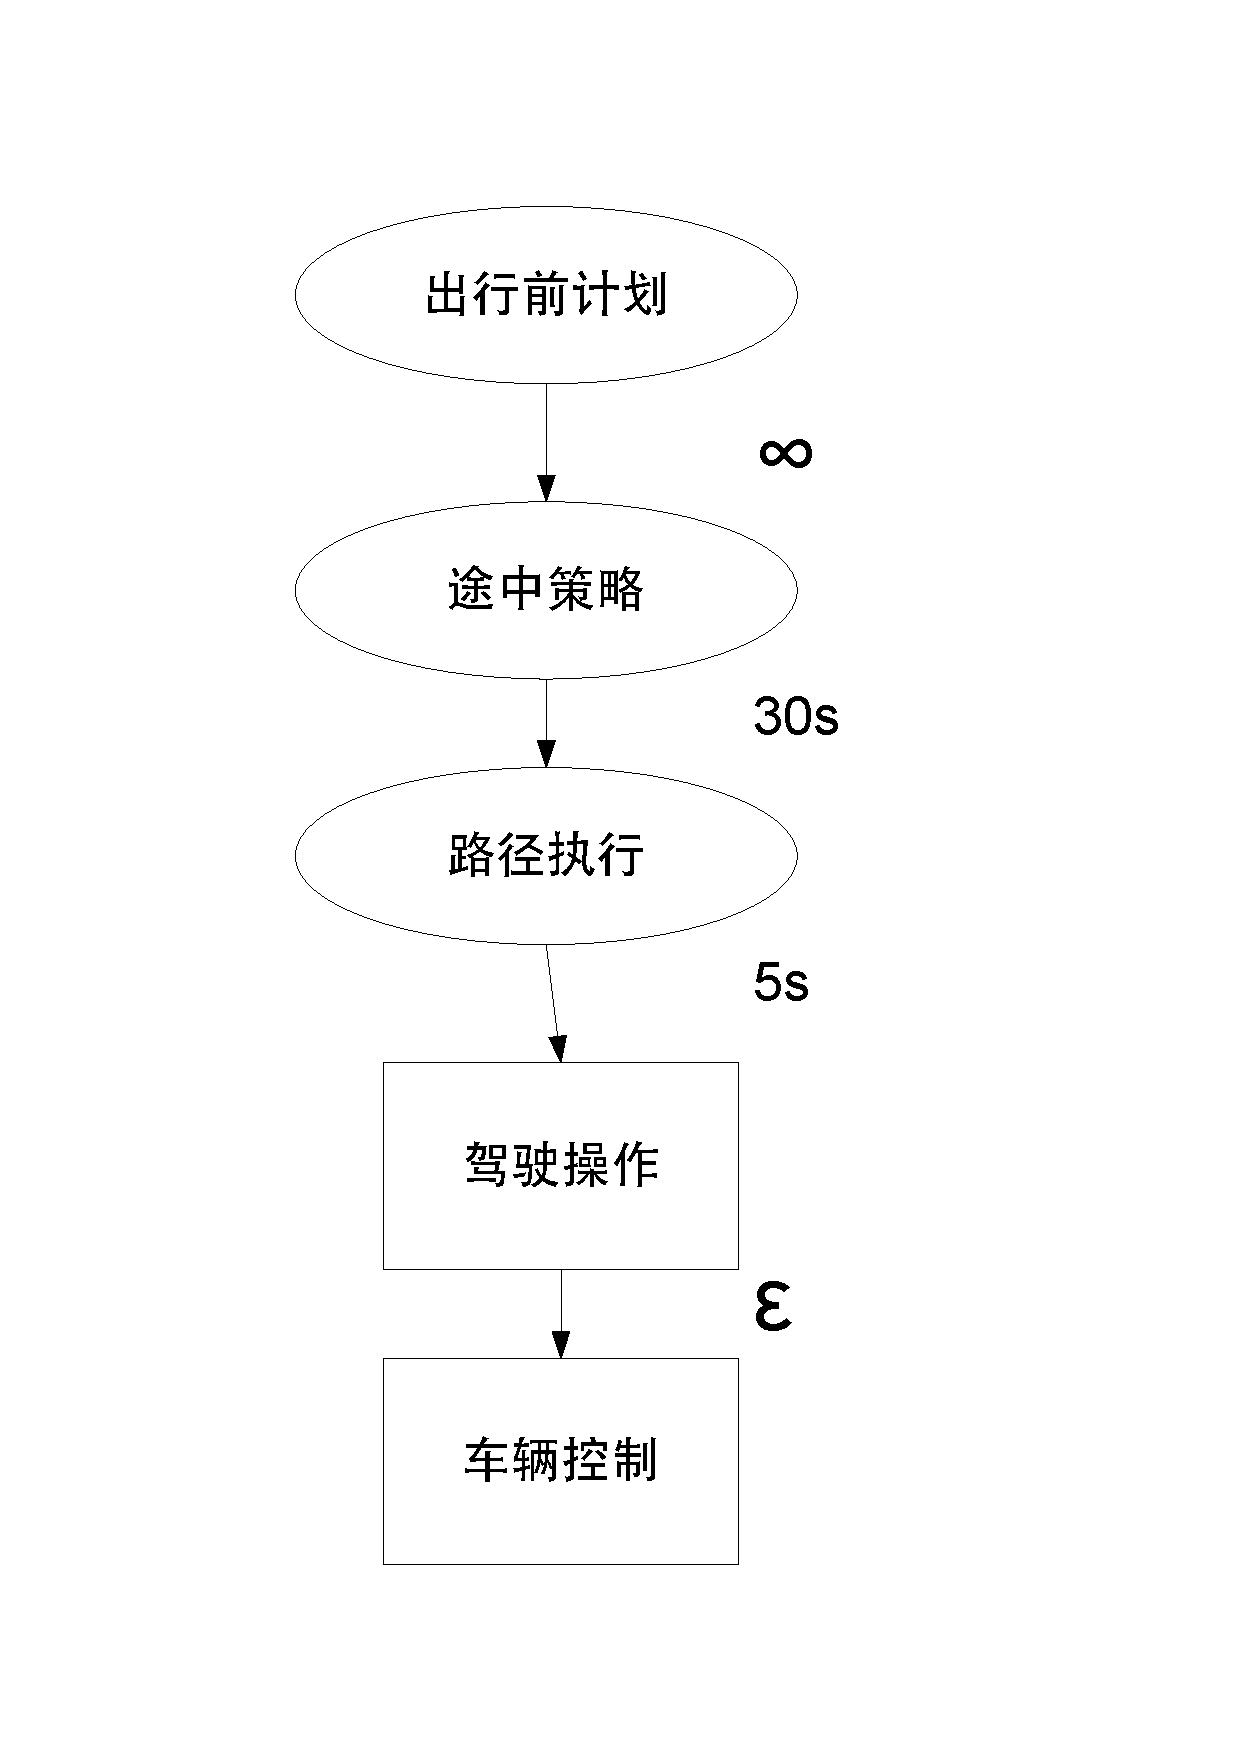
\includegraphics[width=0.3\linewidth]{traveldecision}
	\caption{出行行为层次图\cite{Hranac2004}}
	\label{traveldecision}
\end{figure}

本文所指的驾驶人行为指的是层次4,即驾驶操作这一层次,这也是大多数驾驶人行为模型所研究的层次。

%According to the NGSIM Core Algorithm Analysis Report (Hranac et al. 2004a), 
%travel decisions can be classified into the following categories based on the time scale of 
%application (shown in Figure  1.1): 
%
%1. Pre-trip traveler decisions: These strategic decisions are taken before starting a trip 
%and constitute the pre-trip plan of the traveler. Examples include, deciding whether or not 
%to travel, selecting the time of departure, destination, mode of transportation and route 
%etc.  
%
%2. Strategic en-route traveler decisions:  Once the pre-trip decisions are made, the 
%traveler either executes the originally selected plan without any change, or makes one or 
%more modifications to the initial plan. This category of decisions includes modification of 
%destination, mode or route, parking choice etc.  
%The decisions in category 1 and 2 take over 30 seconds (and in most cases much 
%longer) to make and execute. 
% 
%3. Tactical route execution decisions:  This category deals with traveler decisions that 
%take between 5 and 30 seconds to make and execute. While executing a route from an 
%origin to a destination, a series of tactical maneuvers are performed by drivers based on 
%sub-goals generated from a variety of factors. Examples include, maintaining a desired 
%travel speed, making up lost time from a previous delay, avoiding large trucks, pre-
%positioning to get into the appropriate lane, etc. These broad set of route execution 
%decisions result in a combination of lower-level tactical plans.  
%
%4. Operational driving decisions:  The operational behaviors of travelers include 
%decisions to control their vehicle at a time scale of less than five seconds. These include 
%lane shifting, gap acceptance for executing a lane change or for maneuver at an 
%unsignalized intersection, acceleration/deceleration, queue discharge behavior etc.  
%
%5. Vehicle control decisions: This category deals with driver decisions related to 
%controlling the vehicle at a nanoscopic time-scale level, steering the wheel of the vehicle 
%or pressing the accelerator for example. 
%Driving behavior models encompass the tactical route execution and operational 
%driving decisions. It should be noted that only the actions associated with the operational driving decisions and sometimes the vehicle control decisions are observed. The strategic 
%and tactical plans that lead to that action are generally unobserved or latent.
\section{驾驶人行为的过程}
驾驶人行为可以划分为三个不断交替的过程,感知与信息收集,驾驶决策和对车辆的操控。感知与信息收集过程中,驾驶人主要依靠视觉采集相关的信息,这些信息来源于周围车辆和自身车辆。其中驾驶人只对部分信息变量敏感,包括速度,加速度,跟驰距离,相对速度,以及这些变量的某些函数(如时间间隔)。驾驶人收集到信息后通过采样与整合对这些信息进行解释,这种解释依靠驾驶人的对于车辆动态特性的理解以及其积累的驾驶经验。通过对信息解释的整合处理,最终形成驾驶决策。驾驶决策形成后,驾驶人通过对车辆机件的操作,对车辆的动态施加控制。

而本文所研究的的驾驶人行为特性是指驾驶人通过操控车辆,使得车辆所表现出的一系列特性,而不具体研究驾驶人操控动作。其中驾驶过程框图如\autoref{drv_blockdia}


\begin{figure}[!h]
	\centering
	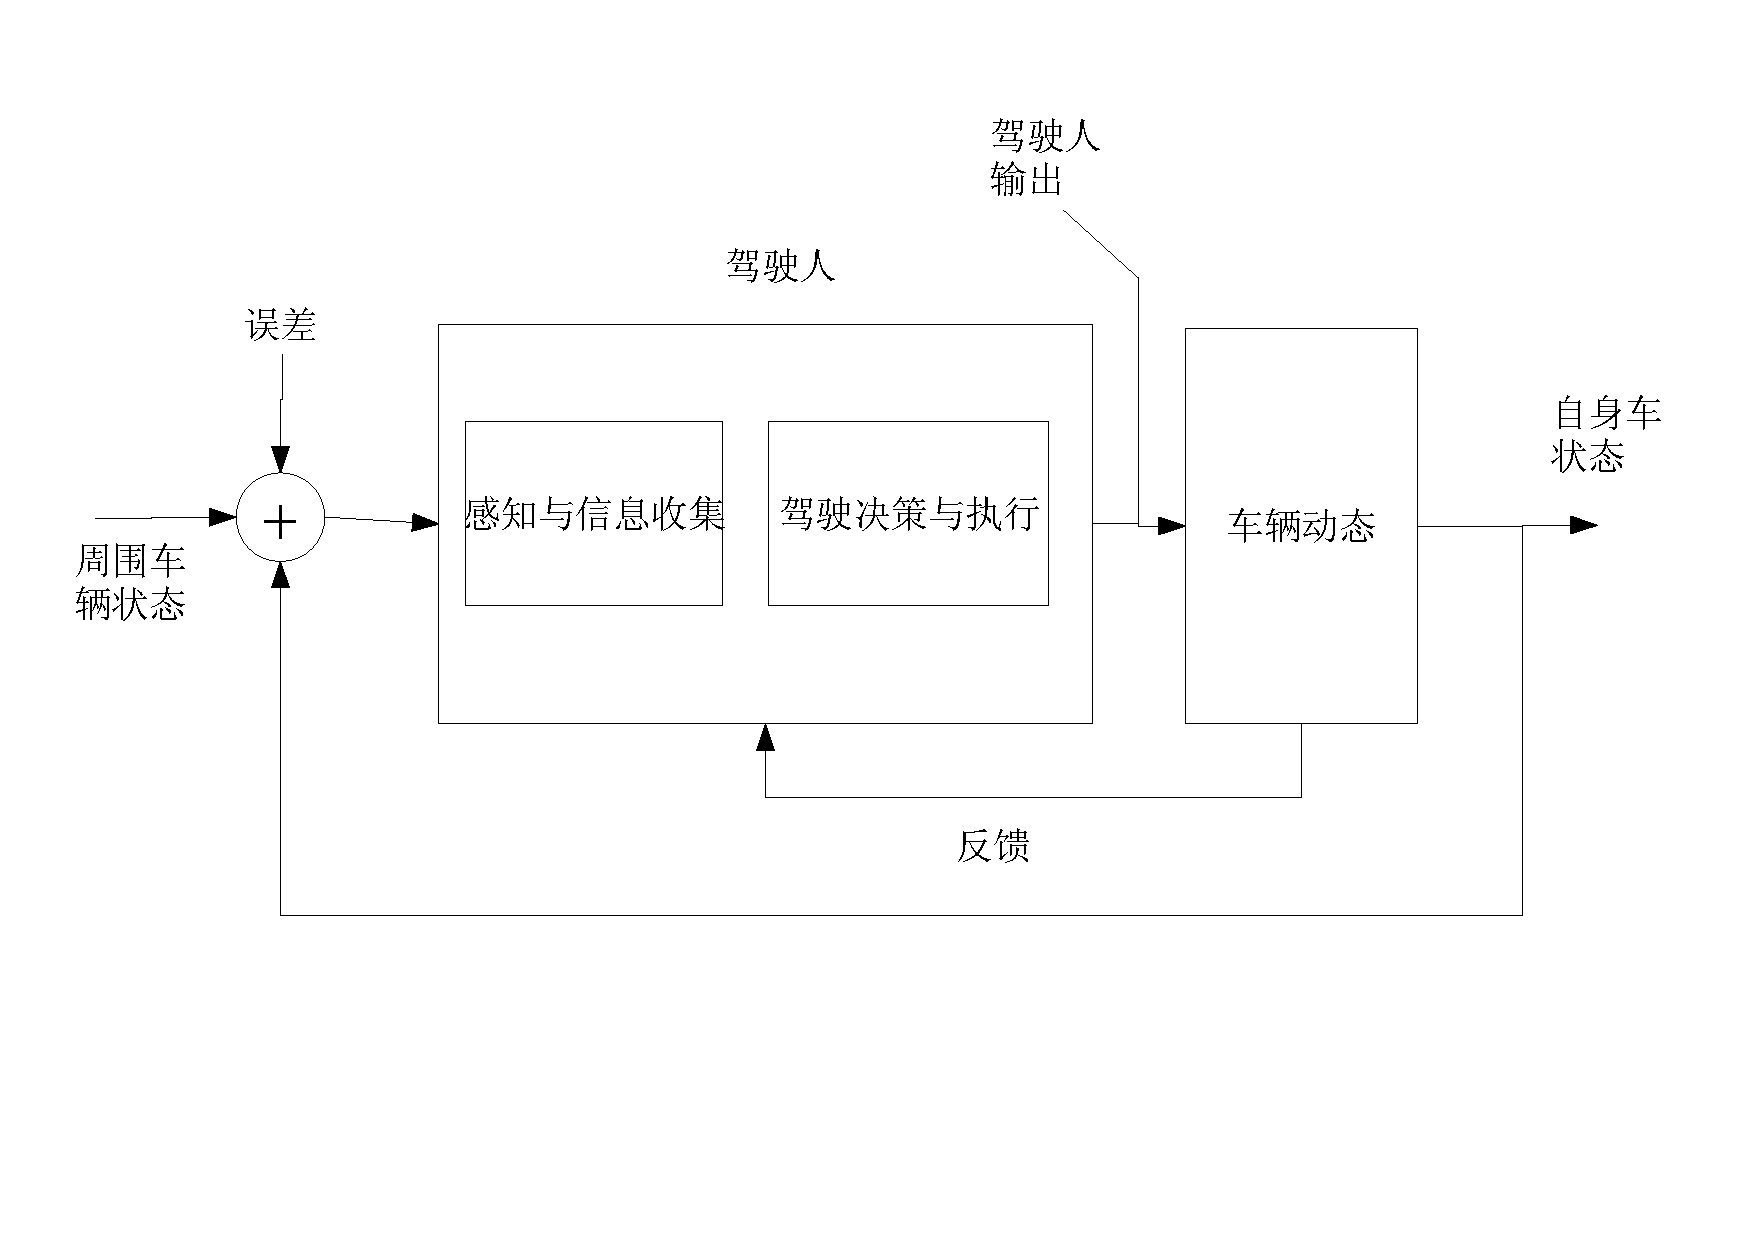
\includegraphics[width=0.5\linewidth]{drv_blockdia}
	\caption{驾驶过程框图}
	\label{drv_blockdia}
\end{figure}
驾驶人行为又可以分为跟驰行为和变道行为,跟驰行为是指驾驶人控制车辆跟随前方车辆保持一定距离,一定速度行驶的行为,这也是驾驶人最常面对的驾驶任务。变道行为是指,驾驶人暂时脱离跟驰状态,为了超车、转向或者提升驾驶条件而变换车道的行为。

两种行为事实上存在紧密联系,但是现阶段研究中仍然分别对这两种行为独立地进行分析,这种两者相对独立的假设便于开展研究,并且有利于交通流模拟系统的实现。本章中将对驾驶人的跟驰和变道行为特性的含义分别进行阐述。
%\begin{table}[htbp]
% \centering
% \caption{Add caption}
% \begin{tabular}{cccc}
%   \addlinespace
%    \toprule
%    Face database & Yale  & Caltech & ORL \\
%    \midrule
%    Number of training & \multicolumn{ 1}{c}{5} & \multicolumn{ 1}{c}{3} & \multicolumn{ 1}{c}{3} \\
%    samples per class  & \multicolumn{ 1}{c}{} & \multicolumn{ 1}{c}{} & \multicolumn{ 1}{c}{} \\
%    \bottomrule
%    \end{tabular}
%  \label{tab:addlabel}
%\end{table}

\section{跟驰行为特性}


\subsection{跟驰行为特性参数}
描述微观的驾驶人跟驰行为时,对于每一个人车单元DVU(driver-vehicle-unit)(也就是外在所表现出来的车辆,下文不再对此进行区分)有若干的特性参数来反映驾驶人的行为,这些参数包括两类,一类是可以直接测量或经由简单计算所得的变量,直接测量的变量包括车辆的即时速度,即时加速度,相对速度和跟驰距离。由直接测量变量经过计算得出的变量,包括跟车对的时间间隔。第二类是不可直接或很难测得也不可经由简单计算得出的变量,这些变量也反映了驾驶人行为的重要特征,因无法直接测量,需要根据前一类变量通过估计的方法得出合理的近似值,包括驾驶人的期望速度,期望跟驰距离,反应时间,期望时间间隔。

\subsubsection{速度}
车辆速度是$v$是跟驰过程中最为基本的变量,速度为车辆单位时间内的位移,在水平面上包括沿道路轴向和横向的速度分量。在跟驰过程中,车辆的沿道路纵向速度为影响跟驰车辆对相互作用的主要因素,而在正常的跟驰过程中车辆的沿道路横向速度相对轴向很小,因此在数量上,车辆速度与车辆沿道路轴向速度几乎总是非常相近。若以道路上一点作为起点,将车辆前保险杠点的沿道路方向的位移$X$看作是时间的函数,则速度为沿道路方向的位移的一阶导数,即$v=\dot{X}$。

\subsubsection{加速度}
加速度与速度类似的包括沿道路纵向和横向的上分量,加速度是速度的一阶导数,是位移的二阶导数,即$a=\dot{v}=\ddot{X}$。按照加速度可将车辆的运行状态分为三类,$a>0$时为加速状态,$a<0$时为减速状态,$a=0$时为巡航状态,驾驶人通过控制油门踏板和减速踏板的开合度改变车辆的加速度。

\subsubsection{相对速度}
相对速度为跟车对的速度差,为引导车辆速度值减去跟驰车辆速度值。以$v_{n-1}$表示引导车辆速度,以$v_n$表示跟驰车辆速度,则相对速度$v_r=v_{n-1}-v_n$。一般认为相对速度是跟驰过程中驾驶人接受的主要刺激,驾驶人根据前后车辆的速度差相应的调整自身车辆的行驶状态。

\subsubsection{跟驰距离与车头间距}
车头间距是跟车对车头之间的距离$\Delta X_n=X_{n-1}-X_n$。跟驰距离则指车头间距减去前车车身的长度$l_{n-1}$,即$D_n=\Delta X_n-l_{n-1}=X_{n-1}-X_n-l_{n-1}$。跟车实验中一般容易测得的是跟车距离,一般认为当跟驰距离大于或等于最坏条件下的安全距离能保证不发生追尾事故,其中最坏条件下的安全距离是指前车t时刻瞬时停止的情况下,跟驰车辆从t时刻开始从反应到制动直至完全停下所运动的距离。而跟驰模型中则更多的使用车头间距,平均的车头间距反映了交通流的密度情况。
%而最小安全距离的根据跟车对之间相对速度的关系和不同的定义而变化。

\subsubsection{时间间隔与车头时距}
车头时距为跟驰车辆车头$t$时刻在速度不变的情况下到达$t$时刻前车车头位置所需要的时间,$h_t=\frac{X_{n-1}-X_n}{v_n}$,平均车头时距反映了交通流的流量情况。时间间隔为跟驰车辆车头$t$时刻在速度不变的情况下到达$t$时刻前车后保险杠位置所需要的时间,$g_t=\frac{X_{n-1}-X_n-l_{n-1}}{v_n}$,时间间隔体现了驾驶人出于安全性考虑而保留的一定的可用于驾驶操作的余地。

\subsubsection{反应时间}
反应时间是驾驶人从外界条件发生改变的一刻开始到其控制自身车辆使其运动发生相应改变所需要的时间,此处反应时间指人车单元即车辆的总反应时间$t_l$,包括驾驶人的感知时间$t_p$,反应操作时间$t_r$和车辆机械延迟时间$t_m$,即$t_l=t_p+t_r+t_m$。


\subsubsection{期望参数}
%Gipps ?Newell模型里的期望速度?
考虑期望参数即打破了驾驶人跟驰过程是完全反应式行为的假设,期望参数考虑了驾驶人的主观愿望,也就是说驾驶人在跟驰过程中会期望达到理想的跟驰状态,并在受限制的条件下对跟驰行为进行相应的调整。理想的跟驰状态由期望参数体现,具体期望参数主要有期望速度、期望车头间距和期望时间间隔等。不同的期望参数有其特定的含义,一般意义上驾驶人所期望的跟车行驶状态要满足驾驶人对于效率性,安全性等方面的需求。


%期望速度(又称为心理速度,以符号$v_{dsr}$表示)是指在特定的道路条件下,车辆行驶过程中不受或基本不受其他车辆约束的条件下其驾驶员心目中希望达到的最高“安全”速度
%
%期望速度有不同的定义(又称为心理速度,以符号$v_{dsr}$表示)是指在特定的道路和交通条件下驾驶员心目中希望达到的合宜的速度。期望速度受到诸多因素的影响,如驾驶人行程的紧迫性,驾驶习惯,同时还受到道路线行,交通流状态的约束。
%
%Mclean是第一个定义期望车速的人,他认为:“期望车速是在自由流状态下,驾驶员不受线形约束所选择的运行速度。”

%\subsubsection{期望跟驰距离}
%
%\subsubsection{期望时间间隔}

%\subsubsection{视觉扩张率}


\subsection{跟驰行为的一般模型}
跟驰模型对驾驶人的跟驰行为的目标作出各种假设而简历数学模型。在众多的跟驰模型中影响较为广泛的有如下几类。
\subsubsection{刺激反应模型}

刺激反应模型假设跟驰中驾驶人通过视觉感知与前车的距离以及前车后部面积在视野中的大小变化来判断与前车接近或是离去及其快慢程度,通过接受这一刺激并作出判断,实施操纵从而达到安全而紧密地跟随前车行驶。刺激反应模型的基本形式为,$\text{反应}(t+\Delta t)=\text{敏感度}{\times}\text{刺激}(t)$。其中最为典型的刺激反应模型是Chandler等(1958),Gaziz等(1959,1961)于20世纪在美国通用汽车公司研究实验室开发的一系列模型\cite{Chandler1958,Gazis1959,Gazis1961}。

其中Gaziz等(1961)给出了最一般形式的非线性GM模型\cite{Gazis1961}。非线性GM模型基于如下假设:在时刻$t+\Delta t$跟驰车的反应依赖于跟驰车对刺激的敏感度和引导车所给的刺激强度,刺激强度以引导车与跟驰车之间的相对速度、距离的形式给出,跟驰车的反应通过加速度测得,敏感特性描绘出单位刺激的反应,$\Delta t$为反应时间。GM模型的一般形式如下式:
\begin{equation}
\ddot{X}_{n+1}(t+\Delta t)=\frac{\alpha_{l,m}[\dot{X}_{n+1}(t+\Delta t)]^m}{[X_n(t)-X_{n+1}(t)]^l}\cdot [\dot{X}_n(t)-\dot{X}_{n+1}(t)],
\end{equation}
式中:
\begin{displaymath}
{\begin{aligned}
m&-\text{对速度}\dot{X}_{n+1}(t+\Delta t)\text{的敏感性参数}\\
l&-\text{对车头间距}X_n(t)-X_{n+1}(t)\text{的敏感性参数}\\
\alpha_{l,m}&-\text{常数}\\
\end{aligned}}
\end{displaymath}

\subsubsection{期望参数模型}
%Several models were developed assuming that drivers
%try to attain some desired measure. 
期望参数模型针对GM模型中速度差为零时跟驰距离可能很小的不合理情况,考虑了驾驶人的主观愿望,假设驾驶人在跟驰过程中会期望达到理想的跟驰状态,理想跟驰状态的参数主要有车速,车头间距和车头时距。

Helly模型,Helly(1961)提出驾驶人的反应不仅与相对速度有关,还与期望车头间距与实际车头间距差值有关\cite{Helly1961}。其模型如下:
\begin{equation}
a_n(t)=a_1\Delta V(t-\tau_n)+a_2[\Delta X_n(t-\tau_n)-D_n(t-\tau_n)],
\end{equation}

其中$D_n$是期望车头间距,其大小受到本车速度的影响。Helly模型指出并解决了GM模型中如果两车以相同速度行驶则任何车头间距均可接受的这一缺陷。
% is the desired space headway, which depends on the subject speed.
%This model addresses a deficiency of the GM model that if two vehicles travel
%at the same speed, any value of the spacing between them is acceptable. Bekey
%et al. (1977) develop a similar model from optimal control considerations.

Koshi等(1992)提出了这一模型的非线性版本\cite{M.Koshi1992}. 他们的模型中期望车头间距给出如下:
\begin{equation}
D_n(t-\tau_n)=L_{n-1}+V_n(t-\tau_n)T,
\end{equation}
其中$L_{n-1}$为引导车长度,$T$是假定为恒定的期望车头时距。

Addison和Low(1998)以及Low和Addison(1998)将车头间距项加入GM模型提出了新的模型\cite{Addison1998,Low1998}。
%propose a model that
%combines a desired spacing term with the traditional GM term: 
%m
\begin{equation}
a_n(t)=a_1\frac{V_n(t)^m\Delta V_n(t-\tau_n)}{\Delta X_n(t-\tau_n)^l}+a_2(\Delta X_n(t-\tau_n)-D_n(t-\tau_n))^3,
\end{equation}
其期望车头间距的形式给出如下:
\begin{equation}
D_n(t-\tau)=\lambda V_n(t-\tau),
\end{equation}

\subsubsection{优化速度模型}
优化速度模型假设驾驶人在跟驰过程中根据车辆运动关系有使用最优速度的趋势。

Newell(1961)研究了速度与车头间距的关系,其假设为车速为车头间距的非线性函数\cite{Newell1961}:
\begin{equation}
V_n(t)=G_n[\Delta X_n(t-\tau)],
\end{equation}
函数$G_n$的形式体现了驾驶人的跟驰行为,Newell(1961)研究了$G_n$的具体形式\cite{Newell1961}:
\begin{equation}
V_n(t)=V_{max}\left[1-exp\left(\frac{-\lambda}{V_{max}}(\Delta X_n(t-\tau)+D)\right)\right],
\end{equation}
其中$V_{max},\lambda$和$D$为参数。$V_{max}$和$\lambda$可以相应的理解为最高车速和最小车头间距。

Bando等(1995)假设驾驶人施加的加速度跟其实际车辆速度与期望速度的差值成正比,而期望速度由与前车间距决定\cite{Bando1995}。模型忽略了反应时间,其形式如下:
% assume that the acceleration drivers apply is proportional to
%the deviation of their actual speed from a desired speed, which depends on the
%leader spacing. Reaction times are ignored. The model is given by: 
\begin{equation}
a_n(t)=\alpha[DV_n(t)-V_n(t)],
\end{equation}
%where DVn
%(t) is the desired speed. The following function was proposed, but no
%behavioural or empirical justification was presented: 
其中$DV_n(t)$为期望车速,其函数给出如下,但未给出理论或实际观测的证明。

\begin{equation}
DV_n(t)=\mathrm{tan}h(\Delta X_n(t)-2)+\mathrm{tan}h(2),
\end{equation}

\subsubsection{安全距离模型}
Gipps(1981)\cite{Gipps1981}提出了基于安全跟驰距离的模型,其模型假设驾驶人与前车保持一定的安全从而保证在前车以最大减速度减速的条件下,仍能够在最小停车间距的距离停车。其跟驰状态下的速度形式如下:

\begin{eqnarray}
&&v_n^{con}(t+T_r)=b^{max}*(\frac{T_r}{2}+\theta)\nonumber\\
&&+\sqrt{(b^{max})^2*(\frac{T_r}{2}+\theta)^2-b^{max}*[2*(\Delta X_{n-1,n}(t)-d)-v_n(t)*T_r-\frac{v_{n-1}(t)^2}{b_{n-1}^{max}}]}
\end{eqnarray}
其中,
\begin{displaymath}
{\begin{aligned}
b^{max}&=\text{最大减速度}\\
d&=\text{停车时的最小车头间距}\\
b_{n-1}^{max}&=\text{驾驶人估计的前车最大减速度}\\
T_r&=\text{反应时间}\\
\theta&=\text{安全反应时间}\\
\end{aligned}}
\end{displaymath}

其自由行驶状态下的速度如下:
\begin{equation}
v_n^{free}(t+T_r)=v_n(t)+2.5*a^{max}*T_r(1-\frac{v_n(t)}{v^*})*\sqrt{0.025+\frac{v_n(t)}{v^*}})
\end{equation}

则驾驶人车辆最终的速度为两者的最小值:
\begin{equation}
v_n(t+T_r)=min(v_n^{con}(t+T_r),v_n^{free}(t+T_r))
\end{equation}

\subsubsection{IDM模型}
Treiber等(2000)\cite{Treiber2000}和Treiber和Helbing(2003)\cite{Treiber2003}假设加速度受到期望速度和期望跟驰距离的影响提出了IDM模型,其形式如下:
% assume that the acceleration is
%affected by both the desired speed and the desired minimum space headway. The
%model also incorporates the impact of vehicle capabilities, but ignores reaction
%time: 
\begin{equation}
a_n(t)=a_{max}\left[1-\left(\frac{V_n(t)}{DV_n(t)}\right)^4-\left(\frac{D_n(t)}{\Delta X_n(t)}\right )^2\right],
\end{equation}
其中$a_{max}$为车辆的最大舒适加速度。$V_n$为实际车速,$DV$为期望速度,$D_n$为期望跟驰距离,$\Delta X_n$为实际跟驰距离。

%其期望车头间距给出如下:
%
%\begin{equation}
%D_n(t)=\Delta X_n^*+V_n(t)T_n(t)+\frac{V_n(t)\Delta V_n(t)}{2\sqrt{a_{max}b_{max}}},
%\end{equation}

驾驶人车辆的加速度由两个部分组成,其趋向自由行驶部分的加速度为:
\begin{equation}
a_{max}\left[1-\left(\frac{V_n(t)}{DV_n(t)}\right)^4\right],
\end{equation}

受前车影响部分的加速度为:
\begin{equation}
-a_{max}\left[\left(\frac{D_n(t)}{\Delta X_n(t)}\right )^2\right],
\end{equation}
当实际的跟驰距离小于期望跟驰距离时,此项成为加速度的主要部分。

其期望车头间距给出如下:
\begin{equation}
D_n(t)=\Delta X_n^*+V_n(t)T_n(t)+\frac{V_n(t)\Delta V_n(t)}{2\sqrt{a_{max}b_{max}}},
\end{equation}
其中$\Delta X_n^*$为停车间距,$T_n$为期望车头时距,当距离较小时$\Delta X_n^*$占期望跟驰距离的主要部分,$T_n$期望车头时距体现了驾驶人对安全跟驰距离的一种期望。$b_{max}$为最大舒适减速度。在大多数情况下将减速度的绝对值限制在其以下。


\subsubsection{各类跟驰模型中对驾驶人行为假设的总结}

各类跟驰模型中对驾驶人的跟驰行为的假设不尽相同,一部分模型将加速度作为驱动驾驶人行为演化的变量:刺激反应模型假设驾驶人的加速度与速度差和车头间距有关,速度差越大、车头间距越小则加速度越大。期望参数模型在刺激反应模型基础上更多地考虑了期望车头间距对驾驶人加速度的影响。IDM模型假设驾驶人的加速度由趋向自由行驶部分和受到前车影响部分组成。

另一部分模型将速度作为驱动驾驶人行为演化的变量:优化速度模型则假设驾驶人根据车头间距来选择合适的最优速度。安全距离模型与优化速度模型类似地假设驾驶人根据车头间距来选择合适的最优速度,而其最优速度的目标为保证不与前车发生碰撞。

从各类跟驰模型对于驾驶人跟驰行为的假设可以看出,驾驶人跟驰过程中影响驾驶人行为的主要包括速度与跟驰距离或车头间距的关系,以及加速度与车辆间相对运动的关系。

%Spacing models.  Spacing models hypothesize that the driver reacts to the leader
%spacing rather than to the relative speed. Newell (1961) assumes that the subject’s
%speed is a non-linear function of the spacing to the leader: 
%The form of the $G_n$
% function specifies the car-following behaviour. Newell (1961)
%studies the properties of the functional form: where $V_{max}$
%, λ  and $D$ are parameters. $V_{max}$
% and $D$ can be interpreted as the maximum speed and the minimum space headway, respectively.
%The acceleration the driver applies, which can be calculated by taking the
%derivatives of both sides of the above equation, corresponds to a non-linear GM
%model, with a sensitivity function that is an exponential function of the spacing.
%Newell studies the macroscopic properties of this model, but does not attempt to
%estimate the model parameters.
%Kometani and Sasaki (1958, 1959) propose a model based on the assumption



%驾驶人的加速选择对于交通流稳定产生影响,目前的研究中考虑了交通流的局部稳定性和渐进稳定性。局部稳定性是指引导车和跟驰车两辆车在特定的速度、加速度初始条件下,驾驶人通过操作是否会发生碰撞的性质,若不会发生碰撞则局部稳定,否则为局部不稳定。而渐近稳定性是指

%关于驾驶人跟驰过程的加速度-相对速度选择特性,
%
%研究发现驾驶人的加速过程以及减速过程中存在不对称性,
%
%的研究表明驾驶人的加速度值会摆动ocsilatory
%
%加速度-相对速度选择还关系到交通流的稳定性stability
%
%所以从实测的角度分析这种选择的差异性
%memory-less?
%
%extende filed of view(multi follow)
%
%planning, anticipation
%
%not myopic state



%\subsection{跟驰行为差异性}

%\subsubsection{跟驰行为内部的差异性}
%multi regime
%Wang Hao的研究表明
%This paper presents a methodology for studying the intra-driver heterogeneity of driving behavior between the acceleration process and the deceleration process with the vehicle trajectory data. The trajectory data collected from peak hours in Dutch Motorway A2 is used in this paper. Some criteria are proposed for the selection of sub-trajectories corresponding to both the acceleration and the deceleration processes of car-following. By applying these sub-trajectories to calibrate three different types of models, namely, the Helly model, the Gipps model and the IDM model, it is found that obvious intra-driver heterogeneities exist in the driving behaviors between the acceleration and deceleration processes of car-following: (a) the average response time of drivers in acceleration process is longer than that in deceleration process according to the prediction of the Helly model and IDM model; (b) drivers are apt to respond more intensively to the surrounding traffic in deceleration process than they do in acceleration process; (c) more than 65\% of drivers involved in this study drive in obviously different styles between the acceleration and the deceleration process. Moreover, the compensation for the response delay from model parameters is observed, and all the three models present low robustness in predicting driving behaviors of one car-following process with the parameters optimized from the data of the other different car-following process. This work not only presents a deep insight into the intra-driver heterogeneity in car-following behaviors, but also suggests some important criteria for car-following modeling.


%\subsubsection{驾驶人之间跟驰行为的差异性}
%\subsubsection{不同跟车对的跟驰行为的差异性}

\section{变道行为特性}

\subsection{变道行为特性参数}
描述微观的驾驶人变道行为时,对于每一个人车单元DVU同样有若干的特性参数来反映驾驶人的行为,与跟驰行为不同的是,变道行为更多时候是驾驶人主动的行为,这也意味着描述变道行为的变量有更多的不可测量的隐藏变量。

%研究驾驶人的变道行为相比跟驰行为要复杂很多。在实际观测中,首先只能观测到驾驶人发生变道的行为,也就是最终接受了间隙的结果。其次驾驶人何时做出了换道的决定通常观测不到,并且换到是连续的过程,当驾驶人作出换道的决定后还有可能寻找其他的间隙或改变换到的决定。

\subsubsection{车道属性}
车道属性包括车道平均速度,车道平均密度,和车道车辆组成等。这些变量是基于效应的模型中驾驶人所选择车道的效用主要的解释变量。驾驶人根据根据自身的观察,一般会对其周围局部的车道属性形成一定的判断。因此车道属性只在一定的时空范围内影响驾驶人的选择车道的效用。

\subsubsection{邻车速度}
驾驶人车辆周围的车辆的速度对于驾驶人的变道行为存在影响,首先周围车辆的速度影响驾驶人的车道选择,其次在驾驶人的目标车道上的前后车车速与自身车辆的车速差影响驾驶人的最小接受间隙。

\subsubsection{间隙}
间隙是指驾驶人在变道间隙接受过程中在与其相邻的目标车道上假设其变道后,前向和后向的净间距$G_f$和$G_b$,其示意图如\autoref{gap_accpet}。当目标车道上的车辆与驾驶人车辆在沿道路方向存在重叠时,间隙可为负值。
间隙接受示意图如\autoref{gap_accpet}
\begin{figure}[htpb]
	\centering
	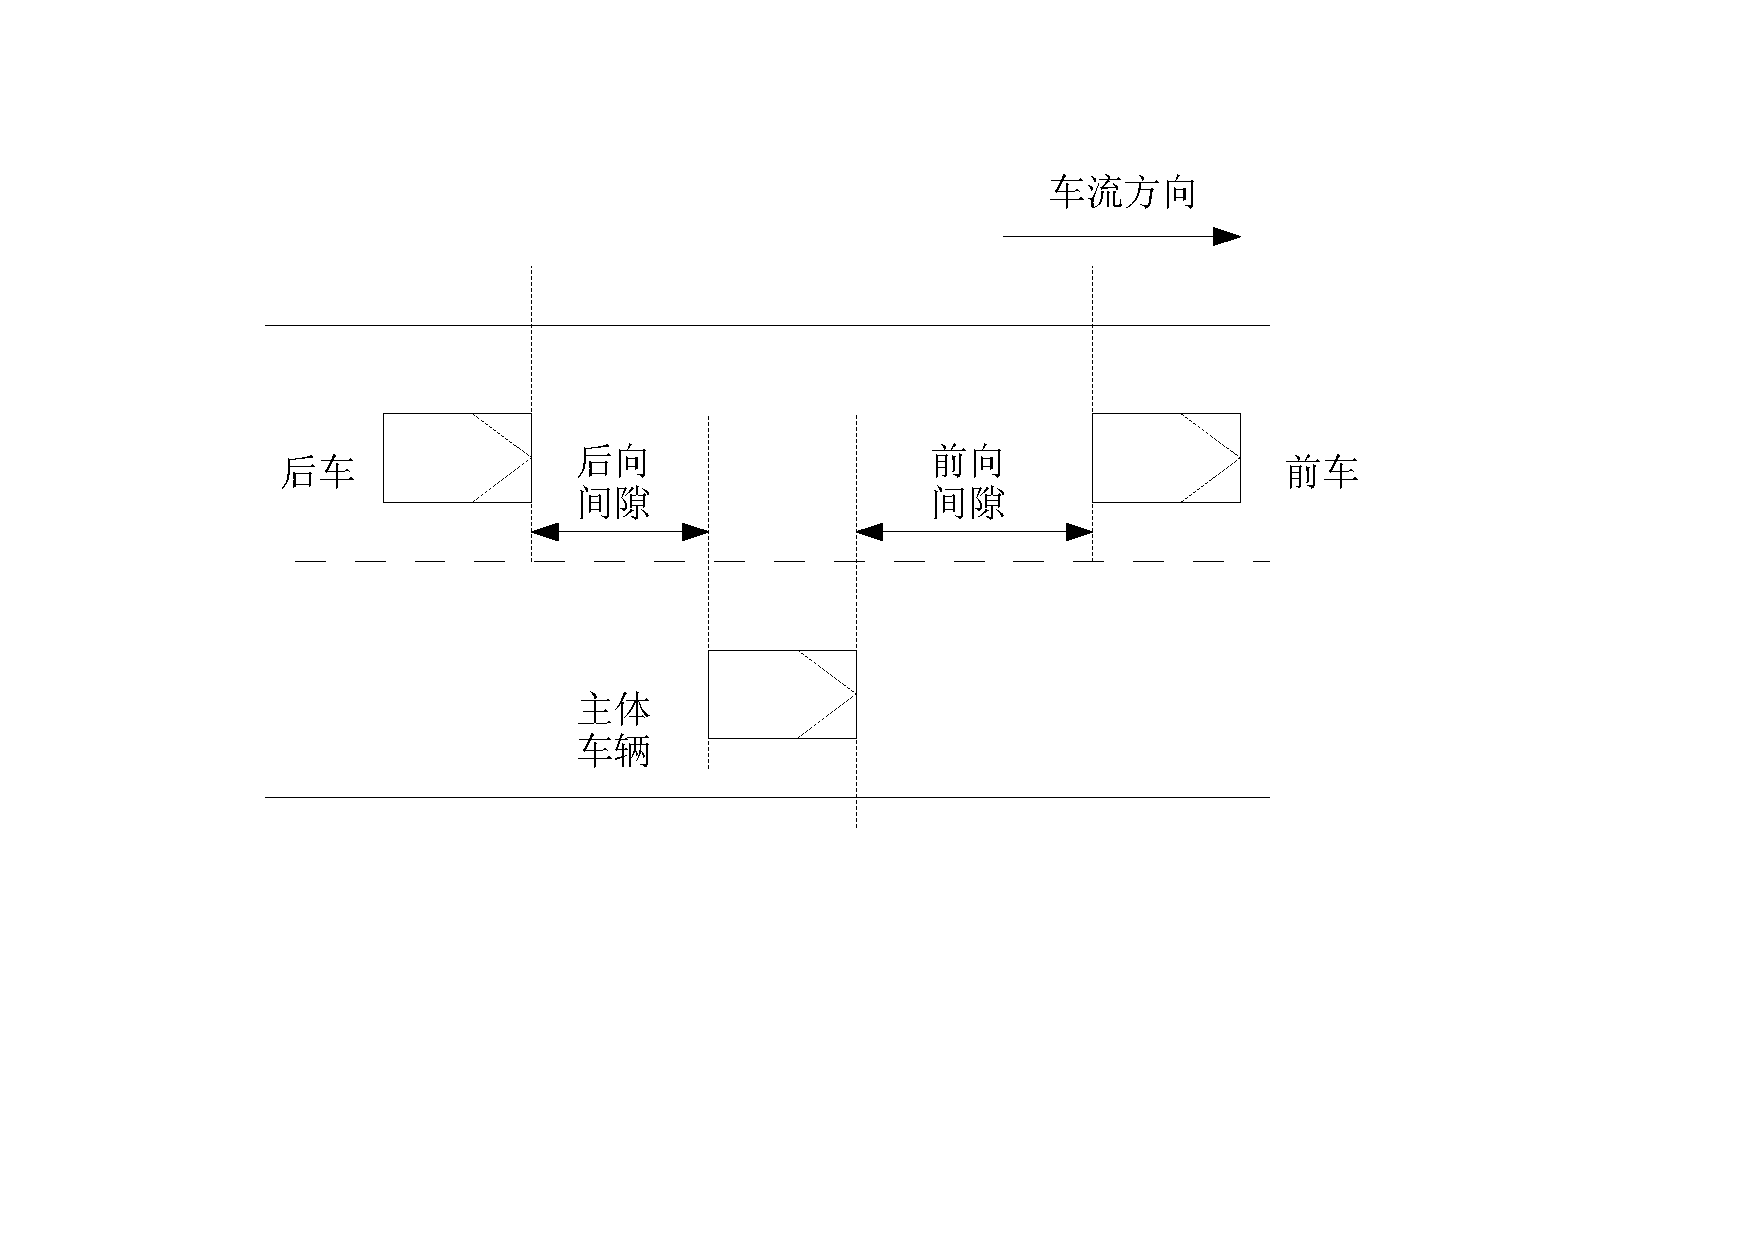
\includegraphics[totalheight=10cm]{gap_accpet}
	\caption{间隙接受示意图}
	\label{gap_accpet}
\end{figure}

\subsubsection{最小接受间隙}
最小接受间隙是指在驾驶人的间隙接受过程中,驾驶人最小的可接受间隙,当实际间隙大于最小接受间隙时则接受间隙进行变道,否则就拒绝间隙保持原车道行驶。
%目前的研究中对驾驶人的最小接受间隙分布进行了分析。

%\subsubsection{加速度改变}
%加速度改变是MOBIL模型中的驾驶人的效用函数,是指驾驶人在假设变换到目标车道以后可以获得的加速度改变(通常是增加)。
%
%\subsubsection{礼让系数}
%礼让系数

\subsection{变道行为的一般模型}
%目前描述变道行为的模型主要有两类,一类是基于车道效用和间隙接受的模型,另一类为MOBIL模型。
变道行为可分为两个阶段,第一阶段选择车道,如果选择车道非现行车道则进行第二阶段执行变道。两个阶段对应的模型分别为目标车道模型和间隙接受模型。
\subsubsection{车道选择模型}

Gipps(1986)最早提出了用于微观仿真的变道模型\cite{Gipps1986}。其模型考虑变道的必要性,可能性和安全性。驾驶人行为考虑两条最基本的原则:保持理想的速度和保持在正确的车道上从而进行计划的转向操作。

Halati等(1997)在CORSIM中提出了MLC和DLC的区别\cite{Halati1997}。按照迫切程度,变道行为可分为MLC(mandatory lane change)强制变道和DLC(discretionary lane change)选择变道,MLC强制变道指驾驶人按照行驶计划的路径必须选择某条车道时的变道行为(例如左转必须使用左转车道或下游拥堵),DLC选择变道则指驾驶人为了追求更为有利的驾驶条件而相对自由进行选择的变道行为。




 


%The first lane-changing model intended for micro-simulation tools was introduced by 
%Gipps (1986). The model considers the necessity, desirability and safety of lane-changes. 
%Drivers’ behavior is governed by two basic considerations: maintaining a desired speed 
%and being in the correct lane for an intended turning maneuver. The distance to the 
%intended turn defines which zone the driver is in and which of the considerations are 
%active. When the turn is far away it has no effect on the behavior and the driver 
%concentrates on maintaining a desired speed. In the middle zone, lane-changes will only 
%be considered to the turning lanes or lanes that are adjacent to them. Close to the turn, the 
%driver focuses on keeping the correct lane and ignores other considerations. The zones are 
%defined deterministically, ignoring variation between drivers and inconsistencies in the 
%behavior of a driver over time. When more then one lane is acceptable the conflict is 
%resolved deterministically by a priority system considering locations of obstructions, 
%presence of heavy vehicles and potential speed gain. No framework for rigor estimation 
%of the model’s parameters was proposed.  
Yang和Koutsopoulos(1996)在MITSIM中实现了一个基于规则的变道模型\cite{Yang1996}。模型中同样区分了MLC和DLC。驾驶人当需要按计划行驶至下一个连接,绕开下游的拥堵,遵守车道使用规则时进行MLC强制变道,其目标冲突通过概率的效用最大化模型解决。而当驾驶人认为引导车速度低于期望速度时考虑进行选择变道DLC,随后驾驶人寻求机会变换到相邻的车道以提高车速。其与以往模型不同之处在于车道选择基于随机的效用模型,体现了驾驶人权衡不同因素(比如速度优势,重车,汇如交通等)对车道选择的影响。
%implemented a rule based lane-changing model in 
%MITSIM where lane changes are classified as MLC and DLC. Drivers perform MLC to 
%connect to the next link on their path, bypass a downstream lane blockage, obey lane-use 
%regulations and respond to lane-use signs and variable message signs. Conflicting goals 
%are resolved probabilistically using utility maximization models. DLC are considered when the speed of the leader is below a desired speed. The driver then checks the 
%opportunity to increase speed by moving to a neighbor lane.  

Ahmed等(1996)和Ahmed(1999)提出了一个基于效用的包含MLC和DLC的通用的模型框架\cite{Ahmed1996,Ahmed1999}。变道过程分三步:决策进行变道,目标车道选择和间隙接受。当不存在MLC条件或驾驶人决定不执行MLC时,进而分两步考虑DLC。首先驾驶人检查自身车道的驾驶条件是否达到满意的程度,这取决于自身车速与期望车速的差值。如果驾驶人对自身车道的驾驶条件不满意,则驾驶人比较自身车道与相邻车道的驾驶条件,其中相邻车道的效用受到车道上的前向和后向车辆车速的影响。
 
%develop a general utility-based framework that captures both MLC and DLC situations. The lane-changing process is modelled with three steps: a decision to consider a lane change, a choiceof a target lane, and the acceptance of gaps in the target lane. If an MLC situationdoes not apply or the driver chooses not to respond to it, a decision whether to consider a DLC is made using a two-step process. First, drivers examine theirsatisfaction with driving conditions in the current lane, which is affected by the difference between the subject speed and its desired speed. The model also captures differences in the behaviour of heavy vehiclesand the effect of the presence of a tailgating vehicle. If the driving conditions in the current lane are not satisfactory, the driver evaluates conditions in neighbouring lanes and in the current lane in order to choose the target lane. The utilities of neighbouring lanes are affected by the speeds of the lead and lag vehicles in these lanes and the current and desired speed of the subject vehicle. A gap-acceptance model is also included within the lane-changing framework. 


Ben-Akiva等(2006)总结了驾驶人一般的车道选择的逻辑\cite{Ben-AkivaM.2006}。
驾驶人一般的变道逻辑图如\autoref{lc_logic}
\begin{figure}[htpb]
	\centering
	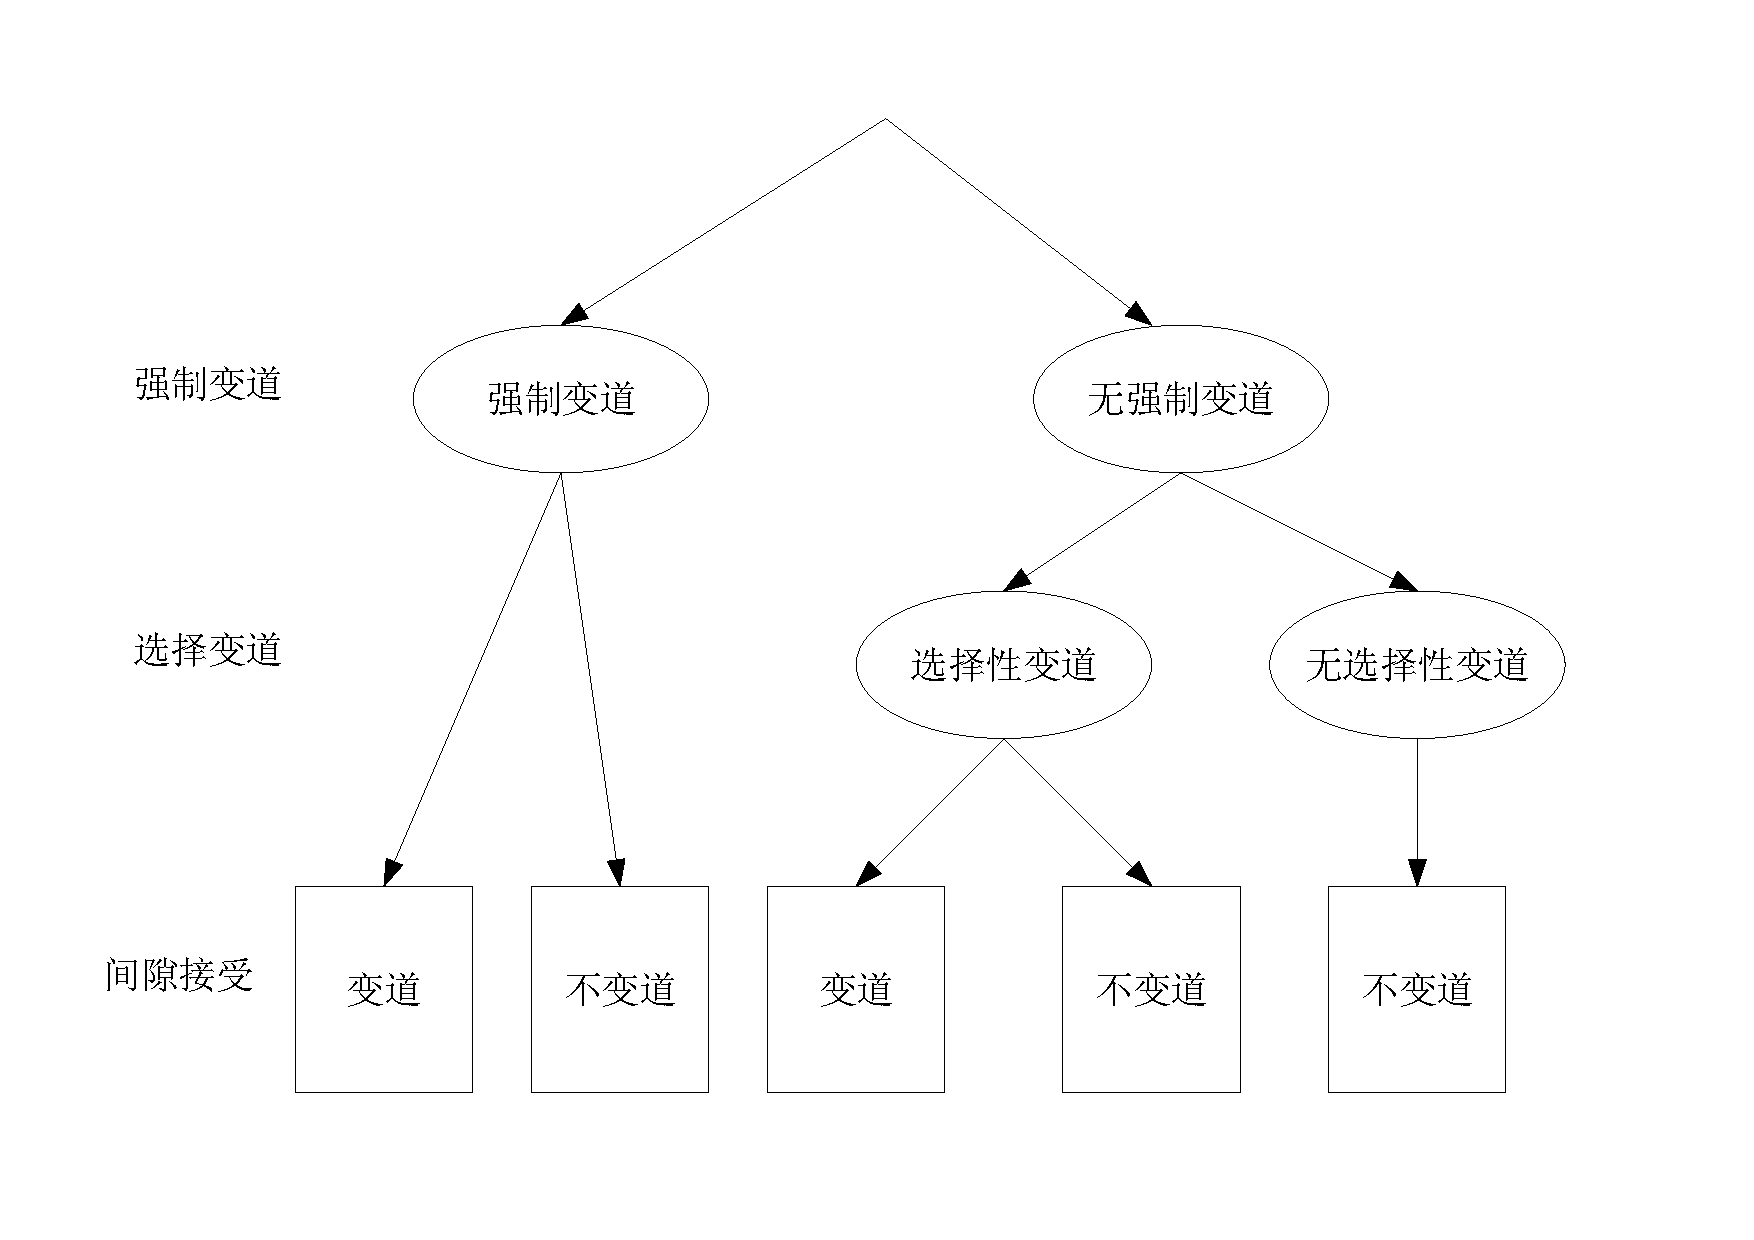
\includegraphics[width=0.4\linewidth]{lc_logic}
	\caption{变道逻辑图}
	\label{lc_logic}
\end{figure}


Toledo等(2005)提出了明确目标车道的车道选择模型,该模型基于效用理论并综合考虑了MLC和DLC,驾驶人选择效用最高的车道作为目标车道。目标车道的选择集包含所有驾驶人可能使用的车道,各条车道的效用函数形式如下:
\begin{flalign}
U_{int}^{TL}=\beta_{i}^{TL}X_{int}^{TL}+\alpha_{i}^{TL}v_n+e_{int}^{TL}\nonumber \\
\begin{split}
\forall i \in \mathrm{\{lane 1, lane 2, lane 3, lane 4, ...\}},
\end{split}
\end{flalign}
其中\\
\begin{displaymath}
{\begin{aligned}
U_{int}^{TL}&-\text{驾驶人}n\text{在时刻}t\text{选择车道}i\text{为目标车道的效用} \\
X_{int}^{TL}&-\text{影响车道}i\text{效用的解释变量构成的向量}\\
\beta_{i}^{TL}&-\text{与}X_{int}^{TL}\text{相对应的参数}\\
v_n&-\text{与驾驶人个体特征相关的解释变量构成的向量}\\
\alpha_{i}^{TL}&-\text{与}v_n\text{相对应的参数}\\
e_{int}^{TL}&-\text{影响驾驶人}n\text{在时刻}t\text{选择}i\text{车道效用的随机项}\\
\end{aligned}}
\end{displaymath}

模型中目标车道的效用受到车道属性(如密度,速度),以及与路径计划相关变量(如到下一个路径中指定车道的距离)的影响。除此之外,驾驶人车辆所处的车道位置也对车道选择产生影响,并在模型中通过需要变道的次数来反映。
%The target lane utilities are affected by the lane attributes, such as
%the density and the speed of traffic in the lane and the presence of
%heavy vehicles, and variables that relate to the path plan, such as the
%distance to a point where the driver needs to be in a specific lane and
%the number of lane changes required to go from the target lane to the
%correct lane. In addition, the vehicle’s current lane and position may
%affect the target lane choice through variables that capture the num-
%ber of lane changes from the current lane to the target lane that are
%required and the spatial relations of the subject vehicle to the vehicles
%around it.
%The driver chooses as the target lane the lane with the highest utility.
%Different choice models are obtained, depending on the assumption
%made about the distributions of the random term ?
%TL
%int
%. If it is assumed
%that they are independently and identically Gumbel distributed, target
%lane choice probabilities (P), conditional on the individual specific
%error term, are given by a multinomial logit model:

\subsubsection{间隙接受模型}

Gipps(1986)假定驾驶人分别考虑前向间隙和后向间隙,两者必须同时满足相应条件,驾驶人才接受间隙。对于间隙的评价是通过计算,本车变道后跟随前车以及购车跟随本车所需要采取的减速值,如果所需减速值小于一定阈值则接受间隙\cite{Gipps1986}。

Kita(1993)对于高速公路匝道汇入处的间隙接受行为用Logit模型进行了估计,并发现重要的影响因素包括,间隙的长度,汇入车辆速度与主线速度差值以及到加速车道末端的距离\cite{Kita1993}。

Ahmed等(1996)假设前向和后向间隙都必须被接受,在其模型中假设最小接受间隙符合对数正态分布,Ahmed等给出了最小间隙的形式,并可以保证其值非负\cite{Ahmed1996}。其形式如下:
\begin{flalign}
ln(G_{nt}^{gd,cr})=\beta^{g^t}+\alpha^gv_n+\epsilon_{nt}^{gd}\nonumber \\
\begin{split}
g \in \mathrm{\{lead, lag\}},d \in \mathrm{\{right, left\}}
\end{split}
\end{flalign}
其中\\
\begin{displaymath}
{\begin{aligned}
G_{nt}^{gd,cr}&-\text{朝着方向}d\text{变道的最小接受间隙} \\
X_{nt}^{gd}&-\text{解释变量构成的向量}\\
\beta^{g}&-\text{与}X_{nt}^{gd}\text{相对应的参数}\\
\epsilon_{nt}^{gd}&-\text{随机项,}\epsilon_{nt}^{gd}\sim N(0,\sigma_{g}^{2})\\
\alpha^{g}&-\text{与驾驶人个体特征有关的随机量}v_n\text{相对应的参数}\\
\end{aligned}}
\end{displaymath}

假设驾驶人比较真实的前后向间隙与相宜的最小接受间隙,当真实的间隙大于最小接受间隙则接受,否则就拒绝。

%In the context of lane changing, Gipps (1986) assumes that drivers consider the
%lead gap and the lag gap separately, and that both gaps must be acceptable. Gaps
%are evaluated in terms of the deceleration required by the subject vehicle in order
%to follow the new leader and by the new lag to follow the subject vehicle. The
%required decelerations are acceptable if they are smaller than a threshold, which
%reflects vehicle capabilities and the urgency of the lane change. Kita (1993) esti-
%mates a logit gap-acceptance model for the case of vehicles merging to a freeway
%from a ramp. He finds that important factors are the length of the available gap,
%the relative speed of the subject with respect to mainline vehicles, and the remain-
%ing distance to the end of the acceleration lane. Ahmed et al. (1996), within the
%framework of the lane-changing model described above, assume that both the
%lead and lag gaps must be accepted. The critical gap functional form guarantees
%that it is always non-negative: 
%
%The gap acceptance model captures a driver’s choice whether the
%available gap in the adjacent lane in the change direction can be used
%to complete the lane change or not. The driver evaluates the available
%lead and lag gaps, which are defined by the clear spacing between the
%rear of the lead vehicle and the front of the subject vehicle and between
%the rear of the subject vehicle and the front of the lag vehicle, respec-
%tively. The lead and lag vehicles and the gaps that they define are
%shown in Figure 3.
%The driver compares the available space lead and lag gaps with the
%corresponding critical gaps, which are the minimum acceptable space
%gaps. An available gap is acceptable if it is greater than the critical
%gap. Critical gaps are modeled as random variables. Their means are
%functions of explanatory variables. The individual specific error term
%captures correlations between the critical gaps of the same driver
%over time. Critical gaps are assumed to follow lognormal distributions
%to ensure that they are always nonnegative:
%
%间隙大于小于时是否接受

%在拥堵的交通条件下
%In heavily congested traffic conditions acceptable gaps may not be available.
%Ahmed (1999) develops a forced merging model for such situations that
%assumes that drivers change lanes either through courtesy yielding of the lag
%vehicle or by forcing the lag vehicle to slow down. Important factors affecting
%this behaviour include the lead relative speed, the remaining distance to the
%point the lane change must be completed and the existence of a total clear gap
%in excess of the subject vehicle length. 
%
%MOBIL模型
Kesting等(2007)提出了基于加速度效用的变道模型即MOBIL模型\cite{Kesting2007}。该模型假设变道行为是驾驶人对变道带来的期望自身加速度增加的正面效应以及变道后后车减速的负面效应的权衡。例如,变换到一条空的车道,可以获得更高的加速度并且不妨碍其他车辆,这种情况下的变道是有利的。模型中给出了效用函数的形式来估计变道所带来的正面效应和负面效应。MOBIL模型中的一个重要参数为“礼貌系数”,“礼貌系数”用来体现驾驶人不同的自私程度。但是MOBIL模型只考虑驾驶人每一瞬间是否变道的选择,并且只适用于DLC情况。
%Kesting et al. (2007) presented a lane-changing model
%focusing on the acceleration decisions instead of the gap
%acceptance. This approach frames the lane-changing
%decision as a trade-off between the expected self-
%advantage and the disadvantage imposed on other
%drivers when changing lanes. For example, moving to an
%empty lane, and hence achieving higher speeds, which
%does not hinder other vehicles, is highly preferred. A
%utility function was proposed to estimate the anticipated
%advantages and disadvantages of a prospective lane
%change. 
%One important feature is that the model con-
%siders a “politeness” parameter, which allows varying
%the motivation for lane changing from purely egoistic
%to more selfless. The lane-changing decision is modeled
%according to the utility gained. By this, the model fo-
%cuses on the driver’s final decision—whether to change
%lanes or not—without considering the initiating rea-
%sons. It takes lane changes as instantaneous events, and
%does not account for the previous steps involved in the
%process, such as vehicle speed adjustments in the sub-
%ject/target lane, and vehicle interactions in preparing
%for a lane change. Consequently, the model is applica-
%ble only for the discretionary lane changes in the speed
%advantage scenario, and cannot be used to model the
%mandatory maneuvers.



%\subsection{本文关注的变道行为特性}
%由于变道行为很难大量跟踪观测,且
%本文着重关注驾驶人的变道间隙接受特性


%\section{跟驰行为与变道行为的关联性}
%前文提到跟驰行为与变道行为并非完全相互独立的,驾驶人所做出的各种决策在时间上以及决策空间上都是相互影响的。例如加速度行为可能会受到变道行为以及穿越交叉口的影响。Zhang等(1998)考虑了驾驶人调整加速度进行变道操作,驾驶人可以加速,减速或者停下从而寻找合适的间隙来完成变道操作,同时还考虑了其他车辆减速避让变道车辆的行为\cite{Zhang1998a}。Toledo(2007)考虑了变道对加速度行为的影响,提出了整合的驾驶模型,模型中加速行为划分为三类,保持车道的加速度模型,变车道过程的加速度模型和目标车道加速度模型,三类模型分别对应了三种不同的外界刺激,在变车道过程的加速度模型和目标车道加速度模型中体现了变道行为和加速度行为的相互影响\cite{Toledo2007}。
%
%跟驰行为和变道行为的相互关联还可能是由于驾驶人内在属性的影响,例如激进的驾驶人其采取的加速度较大而可接受的最小间隙相应的较小,因此跟驰行为与变道行为其特性之间存在怎样的联系还有待进一步研究。本文将联系驾驶人性格及安全意识等内在属性,从关联性的角度对进行驾驶人跟驰行为与变道行为的分析,从而为生成驾驶人提供依据。


%
%Interdependencies. In order to model more sophisticated driving behaviour it
%is necessary to account for interdependencies among the various decisions
%drivers make, both over time and across decision dimensions. For example,
%acceleration behaviour may be affected by lane changing or intersection cross-
%ing decisions. Work in this direction has been done by Zhang et al. (1998) and
%Toledo (2002), who consider the effect of lane changing on acceleration behav-
%iour, 



\section{驾驶人行为的差异性}
本文的一个重要假设就是驾驶人行为的差异性,正是由于驾驶人行为的差异性,驾驶人组成情况的改变才可能导致对交通流的影响。

驾驶人行为的差异性有两种含义,一是不同驾驶人之间的行为差异性,二是驾驶人在不同交通条件,生心理条件下的行为差异性。

不同驾驶人之间行为的差异可以由驾驶人驾驶操作的目标、习惯、熟练程度的差异等多种因素造成。而驾驶人自身,在交通条件,生心理条件发生改变时会改变自己的驾驶行为而作出适应性的调整,最典型的现象是驾驶人加减速的不对称性。本文中将基于驾驶人行为差异性的假设,同时考虑驾驶人行为的差异性的两种含义进行研究。
%
%Driver heterogeneity 
%
%It can be assumed that all driver/vehicle combinations apply the same objective, i.e. 
%react to the same stimuli, while only the extents to which these respective stimuli play 
%a role and to which the driver is able to react differ. In modeling language this means 
%that only parameter values are assumed to differ between individual driver/vehicle 
%combinations. 
%
%The extent of heterogeneity may also be assumed more substantial, such that there are 
%also differences between the objectives of driver/vehicle combinations. In this case 
%models following different logics are assumed to apply to different driver/vehicle 
%combinations. 
%
%has a clear impact on the flow specific lane distributions, especially desired speeds are a key 
%point in this sense. Also the role of heterogeneity with respect to other aspects of car-
%following can not simply be neglected. In dense traffic for example, lane changing 
%possibilities decrease considerably forcing vehicles to drive behind each other on the same 
%lane. In this situation it seems reasonable to assume that car-following heterogeneity can 
%influence the resulting traffic flow dynamics
%
%In modeling changes in the longitudinal behavior of a driver again the same options can be 
%identified, i.e. the control objective of a driver can either be assumed to change over time or to 
%remain the same.  
%
%This overview shows that parameters are often separately estimated for 
%accelerating and decelerating cars. In such a study presented in (Treiterer and Myers, 1974) it 
%is found that drivers tend to place more emphasis on both their own velocity and the spacing 
%between themselves and the leading vehicle while decelerating than while accelerating. 
%Intuitively this can be easily interpreted by considering that drivers decelerate to avoid 
%dangerous situations, while drivers accelerate to improve their situation.  

\section{本文关注的驾驶人行为特性}

本文主要关注驾驶人的跟驰行为特性,主要的原因是驾驶人的变道行为量化的观测十分困难,并且很难区分强制变道和非强制变道,虽然变道行为对交通流可能产生显著的影响,由于研究条件的限制本文不再对驾驶人的变道行为特性作更多的讨论。

本文的目的在于研究驾驶人行为特性对交通流的影响,除了研究单独的行为特性参数,将着重关注可能对交通流状态产生显著影响的跟驰行为特性。直观上,速度-跟驰距离特性对于交通流效率有较大影响,而加速度-相对速度特性对于交通流稳定性和安全性有较大影响。这两方面是驾驶人跟驰过程中最为基本的任务,速度和加速度的选择既有本质的区别又存在联系。速度的选择体现了跟驰过程中驾驶人一种相对稳定的需求(例如对于安全性和执行出行计划的需要),加速度的选择则体现了驾驶人跟驰过程中对于驾驶环境的适应以及驾驶状态的改变;而两方面的联系在于,速度-跟驰距离状态的改变需要通过驾驶人施加操作来实现,也就是说速度的改变通过加速度来实现。本文将在实际测量数据的基础上,对驾驶人一般的跟驰行为特性进行研究,以期加深对驾驶人跟驰行为特性的认识。

\subsection{速度-跟驰距离特性}
速度-跟驰距离选择反应了驾驶人跟驰行为特性中相对稳定的部分,一方面,驾驶人根据出行计划,道路条件,交通流条件来选择车速,当车辆的加速度小于一定的阈值时则认为处于稳定的跟驰状态,此时驾驶人根据其选择的车速会与引导车保持一定的安全跟驰距离。另一方面,由于驾驶人对于外界条件的估计存在误差以及对于自身车辆的控制存在不稳定性,车辆的行驶状态会与驾驶人期望的状态出现偏差,驾驶人需要在一定的跟驰距离下调整自身相应的车速。因此驾驶人的速度-跟驰距离选择是一种组合性的选择。
跟驰距离与车头间距相差的部分为引导车的车身长度,跟驰距离与车头间距两者虽不存在固定不变的算术关系,但是两者的相关性是客观存在的。跟驰模型中出于简便的需要一般使用车头间距,而不是实际中更容易测的跟驰距离
%
%本文将在现有研究以及实测数据的基础上对驾驶人的速度-跟驰距离选择特性进行分析,研究其在驾驶人中的差异性,并通过模拟的方法研究其对交通流的影响。

\subsection{加速度-相对运动关系特性}
加速度-相对速度选择反应了驾驶人跟驰行为特性中相对随机的部分。按照刺激反应模型的假设,驾驶人在一定的相对速度下选择相应的合适的加速度。现有的研究中,Herman等(1958)讨论了基于刺激反应模型的交通流局部和渐进稳定性\cite{Herman1959}。结果表明驾驶人的敏感性参数与反应时间的乘积决定了单车道交通流的局部和渐进稳定性。因此驾驶人的加速度-相对速度选择特性对于交通流存在不可忽略的影响。驾驶人的加速度行为的一个重要特征是加速和减速的不对称性,Forbes(1963)发现驾驶人加速过程中的反应要比减速过程中的慢\cite{Forbes1963}。Foote(1965)跟踪观测了隧道中的车队,发现在同样车速下减速车队具有更高的流量\cite{Foote1965}。Newell(1965)解释了驾驶人加减速的不对称性,认为如果前车加速跟随车会空出一段距离再做决定\cite{Newell1965}。

%
%本文将在现有研究以及实测数据的基础上对驾驶人的加速度-相对速度选择特性进行分析,研究其在驾驶人中的差异性,并通过模拟的方法研究其对交通流的影响。

%
%\section{驾驶人行为特性对交通流的影响}
%%\subsection{交通流状态参数}
%%\subsubsection{效率状态参数}
%%\subsubsection{安全性状态参数}
%表征交通流状态的参数主要可分为两类,一类体现交通流的效率性,另一类体现交通流的安全性。交通流效率性参数包括平均速度,流量,通行能力,行程时间等。交通流的安全性参数包括TTC,交通冲突计数,加速度噪音等。具体的参数内容将在第五章进行阐述。
%
%目前关于驾驶人行为特性对交通流的影响主要关注了驾驶人行为特性对交通流效率参数的影响。

%With respect to the influence of heterogeneity on the fundamental diagram, we made a 
%distinction between the influence of driving style heterogeneity and the influence of within 
%driving style heterogeneity. Our simulations indicated that driving style heterogeneity mainly 
%causes the shape of the fundamental diagram to change. Within driving style heterogeneity on 
%the other hand introduces horizontal scatter to the density-speed plane, meaning that the 
%density corresponding to a given speed becomes stochastic and depends on the composition of 
%the sample of vehicles currently present on the roadway. In the presence of within driving 
%style heterogeneity the fundamental diagram thus becomes a two-dimensional plane rather 
%than a single line.  
% 
%Our simulations indicated that the assumed level of heterogeneity can considerably influence 
%platoon stability. We showed, for instance, that a disturbance in the dynamics of the platoon 
%leader amplified when propagating through a platoon characterized by a low level of 
%heterogeneity, while it smoothed when propagating thorough a platoon characterized by a 
%high level of heterogeneity.  How the disturbance propagated from one vehicle in the platoon 
%to the corresponding following vehicle in the platoon, was found to be dependent on the 
%characteristics of the following vehicle. More specific, the considered heterogeneous platoons 
%consisted of “stabilizing” and “destabilizing” vehicles. Consequently, the propagation of the 
%disturbance was found to be dependent on the platoon composition, i.e. the order of vehicles 
%having different characteristics. 
% 
%As flows typically consist of platoons, the simulation results on flow stability were in general 
%in line with the results on platoon stability. That is, we showed that the impact of disturbances 
%created by a speed-limit and an on-ramp decreased obviously when the level of within driving 
%style heterogeneity was increased. We also found that the flow composition, i.e. the order of 
%vehicles having different characteristics, was important for how the disturbance propagated 
%through traffic flow. 
 
%
%可以看到目前目前关于驾驶人行为特性对交通流的影响还很少涉及交通流的安全性参数,本文将通过模拟的方法,从微观和宏观两个方面分析驾驶人行为特性对交通流效率性和安全性的综合影响。


\section{本章小结}
本章主要阐述本文的研究对象和范围,介绍了表征驾驶人行为特性以及交通流状态的参数和主要有影响力的跟驰和变道模型,简要论述了驾驶人行为特性差异性的含义以及本文主要关注驾驶人行为特性。

\chapter{驾驶人行为特性实验}


%\[D = ct/2\]




\section{有关驾驶人行为特性实验方法回顾}

%\begin{equation}
%D = 2R{\rm{asin}}(\sqrt {\sin _{}^2(\frac{{{l_1} - {l_2}}}{2}) + \cos ({l_1})\cos ({l_2}){{\sin }^2}(\frac{{{w_1} - {w_2}}}{2})} )
%\end{equation}

\section{实验设计}
\subsection{实验目的}

调查专业驾驶人与非专业驾驶人在城市路段行车时,采取的驾驶行为的异同,为进一步分析驾驶人行为特性对城市路段交通流的影响提供数据。

\subsection{实验获取的数据}
分别获取单向两车道与三车道上,驾驶人行车过程中,本车与前后车实时保持的距离,即$S_{\text{前}}$、$S_{\text{后}}$;本车的实时速度$V$,前车的实时速度$V_{\text{前}}$;后车的实时速度$V_{\text{后}}$;本车与前车相对速度${\Delta}S_{\text{前}}$;本车与后车相对速度v’后;本车换道频率n,换道时相邻车道提供的前后车距离s换等。


\subsection{实验设备}
实验设备包括小汽车一辆(现代sonata手动档)、车载激光测速测距仪一体化系统一套(车载激光两台、GPS一个、处理机一台)、摄像机一台、笔记本电脑一台。
\begin{table}[htbp]
 \centering
 \caption{试验设备列表}
 \begin{tabular}{cccc}
   \addlinespace
    \toprule
    序号 & 名称  & 构成 & 用途 \\
    \midrule
	1 & 小汽车 & 北京现代sonata手动档 & 实验用车 \\
	2 & 车载激光测速测距仪 & 车载激光(两台)、GPS、处理机 & 获取实时车间距、相对速度 \\
	3 & 摄像机 & 摄像机 & 车辆换道行为监控 \\
	4 & 笔记本电脑 & Thinkpad T40笔记本 & 现场数据采集终端 \\
    \bottomrule
    \end{tabular}
  \label{equipment}
\end{table}

\autoref{equipment}
其中,小汽车选取目前道路上较为常见,比较有代表性的车型,北京现代的sonata领翔 2.0 GL MT,具体参数如表3-2.

\subsection{实验原理}
通过获取实时连续的本车与前后车的距离以及本车的实时速度,可以推算得到本车与前车和后车的相对速度、前后车的实时速度等相关数据,应用摄像机可以得到本车的换道频率,最后经过数据的处理分析,可以得到换道时本车道前后车的距离,以及换道时相邻车道提供的前后车距离等。
\subsubsection{激光测距基本原理}
激光测距仪是指利用射向目标的激光脉冲或连续波激光束测量目标距离的距离测量仪。它由三大部分组成:激光发射机、激光接收机、电源。激光发射机由脉冲激光器、发射光学系统、取样器以及瞄准光学系统组成,其作用是将高峰值功率的激光脉冲射向目标。激光接收机由接受光学系统、光电探测器和放大器、接收电路和计数显示器组成,其作用是接收从目标漫反射回来的激光脉冲回波并计算和显示目标距离。电源用于设备的供电。
激光测距仪的工作原理是利用脉冲激光器向目标发射单次激光脉冲,计数器测量激光脉冲到达目标并由目标 返回到接收机的往返时间,由此运算目标的距离。计算公式为:

\begin{equation}
D = ct/2
\end{equation}

其中$D$是与目标的距离, $c$为光速,$t$是光往返时间。

激光测距仪的工作过程是:首先瞄准目标,然后接通激光电源,起动激光器,通过发射光学系统,向瞄准的目标发射激光脉冲信号。同时,采样器采集发射信号,作为计数器开门的脉冲信号,起动计数器,钟频振荡器向计数器有效的输入钟频脉冲,由目标反射回来的激光回波经过大气传输,进入接收光学系统,作用在光电探测器上,转变为电脉冲信号,经过放大器放大,进入计数器,作为计算器的关门信号,计数器停止技术。计数器从开门到关门期间,所进入的钟频脉冲个数,经过运算得到目标距离,在显示器上显示出来。


\subsubsection{GPS卫星定位系统基本原理}
GPS系统由空间部分、地面监控部分和用户端三个部分组成。
(1)GPS的空间部分:由21颗工作卫星和3颗备用卫星组成,24颗卫星均匀覆盖在地球上空,可以保证地球上所有地点任意时刻都能同时看到至少4颗GPS卫星。
(2)GPS的地面监控部分:地面监控设备的作用是监测和控制卫星上的各种设备是否正常工作,以及卫星是否一直沿着预定轨道运行;另一作用是保持各颗卫星处于同一时间标准——GPS时间系统。GPS地面监控系统包括一个主控站、三个注入站和五个监测站。
(3)GPS的用户端:即是GPS的信号接收机,它能捕获卫星的信号,对所接收的GPS信号进行变换、放大和处理,实时地计算出测点的三维位置、速度和时间。
GPS系统的基本原理是:太空中的卫星在任意时刻都有一个坐标值(已知值),接收机所在位置为未知值,信息在传送过程中,所需耗费的时间,可经由比对卫星时钟与接收机内的时钟计算之,将此时间差值乘以电波传送速度(一般为光速),就可计算出卫星与接收机间的距离,如此就可依三角向量关系来列出一个相关的方程式,每接收到一颗卫星就可列出一个相关的方程式,因此收到至少三颗卫星信号,即可计算出经纬度坐标,收到四颗则加上高程值,五颗以上更可提高准确度。当接收机处于动态时,每一秒钟的坐标数据都在更新中,也就是说接收机会自动不断地接收卫星信号,并实时地计算其所在位置的坐标数据。系统再将获取的空间与时间的数据结合,计算出车辆的实时速度。

\subsubsection{车载GPS定位仪系统工作流程}
驾驶人在道路上行驶时,车载GPS实时接收卫星信号,经过计算获取车辆实时的精度与纬度,然后将数据传导至处理机,经过处理机运算处理后,计算出车辆的实时速度,最后将实时坐标数据与实时车辆速度传到与处理机相连的笔记本电脑中,为后续的数据处理提供原始资料。车载GPS卫星定位仪工作流程如图3-1所示。

\subsubsection{车载激光测距系统}
激光间距测量仪相比其它测距仪,激光测距仪具有测距精度高、测距速度快、轻小灵活、测量距离数字显示、操作简单等优点。下面分别介绍车载激光的硬件系统和软件系统。
(1)硬件系统
车载激光硬件系统包括激光接收发射一体化系统、车载电源线、输出终端(笔记本)及相关配套设施。其中激光发射机、接收机是车载激光系统的主体设备,封装于一台设备中。给设备连接于一台处理机上,处理机经过计算,将获取的数据发送到笔记本电脑上显示,处理机另外外接两条线,一条是车载电源线,与12V的车载电源连接;另一条是数据线缆,与笔记本相连,与笔记本相连的一端采用了USB2.0 to SR232转换接口。硬件系统模式见图3-2。
(2)软件系统
由激光测距工作过程知,脉冲个数的读取及目标距离需要通过运算得到。北京奥泽尔科技有限公司为本次试验专门开发了一个为计算车头间距的激光测距软件。

\subsubsection{仪器安装}
仪器的安装如图3-4所示。一个车载激光固定在实验车辆挡风玻璃后面,中控台中央的位置,激光头向前放置,能够使激光照射到实验车辆前方的物体;另一个车载激光固定在后车窗玻璃以内,激光头向后放置,透过后车窗玻璃使激光能够照射到实验车辆后方的物体;车载GPS固定在车辆中将的位置;处理机和笔记本电脑放置在车辆后排座位上;摄像机固定在实验车辆后排座位靠背的中间位置上,可以通过实验车辆挡风玻璃拍摄到前方的道路交通情况。

\subsubsection{数据处理}
通过实验仪器获取的数据只有实验车辆与前车和后车的实时距离,以及实验车辆的实时经纬度,要得到我们所需要的实验车辆速度、前车相对速度、前车速度、后车相对速度、后车速度等数据,可以通过以下计算得到。
GPS定位仪输出的是WGS-1984经纬度坐标,在此坐标下计算行驶距离的公式为:
\begin{equation}
D = 2R{\rm{asin}}(\sqrt {\sin _{}^2(\frac{{{l_1} - {l_2}}}{2}) + \cos ({l_1})\cos ({l_2}){{\sin }^2}(\frac{{{w_1} - {w_2}}}{2})} )
\end{equation}
其中 $D$(m)为经纬度坐标点( ${l_1},{w_1}$)和(${l_2},{w_2}$)之间的距离, $R$为地球半径,取6378137m。设定GPS每秒钟返回一个数据,当前车辆的瞬时速度 (单位m/s)计算公式为:$v = D'$
设$\Delta t$为记录前后两个坐标点的时间差,本车加速度 $a$($m/s^2$)则通过本车速度计算得到,计算公式为:
\begin{equation}
a = \frac{{{v_1} - {v_2}}}{{\Delta t'}}
\end{equation}
其中$v_1$,$v_2$分别为相邻的两瞬时速度(单位m/s), $\Delta {t'}$为两个瞬时速度的时间差(单位s)。激光测距仪直接输出的是本车车头与前车车尾之间的间距,前车与本车的相对速度 (m/s)计算公式如下:
\begin{equation}
{v_r} = \frac{{{d_2} - {d_1}}}{{\Delta {t^{''}}}}
\end{equation}
其中$d_1$,$d_2$为相邻两个车间距(单位m), $\Delta t''$为两个相邻车间距对应的时间差(单位s),又${v_r} = {v_f} - {v_b}$,其中${v_f}$为前车速度(单位s), ${v_b}$为后车速度(单位s),故前车的速度为:
\begin{equation}
{v_f} = {v_r} + {v_b}
\end{equation}

\subsection{实验方法}
\subsubsection{实验对象}
实验对象分为专业驾驶人与非专业驾驶人,各十五人。其中,专业驾驶人主要选取长期从事驾驶工作,或驾龄7年且累计行程10万公里以上的驾驶人;非专业驾驶人主要选取非特定职业,驾龄不足7年或累计行程不足10万公里的驾驶人。选取的专业驾驶人与非专业驾驶人都尽可能来自各行各业,覆盖各年龄层,男女比例均衡。
\subsubsection{实验路线}
实验路线的选取要注意多项条件。首先,道路条件方面应包含单向两车道城市道路与单向三车道城市道路,且路段上开口较少,有机非分隔带,机动车行驶受非机动车和行人干扰较小,路面情况良好;其次,交通条件方面要有足够大的交通流量,但是不至于造成长时间的拥堵,道路上行驶的车型以小汽车为主。
经过实地调查分析,本实验选取的实验路段为:南京市龙蟠中路-瑞金路-御道街-中山东路一线。其中龙蟠中路为双向六车道;瑞金路东西向为三车道,西东向为两车道;御道街靠近瑞金路一段为双向四车道,靠近中山东路一段为双向六车道;中山东路为双向四车道。该路段全天交通流量均较大且高平峰时流量相差不大,平峰时段车流量满足要求,高峰时段不造成长时间拥堵,车辆跟驰特征明显,比较符合实验要求。具体线路如图3-5所示。

\subsubsection{实验条件}
天气状况良好、无大风大雨、光线充足的情况下,分别在工作日与非工作日的交通流量较大的时候进行实验。所选取的时间段主要在车流量较大但不造成长时间拥堵的时候,能够满足车辆跟驰的要求。经过调查发现,在该路段上,工作日与非工作日的交通流量变化不大,交通流量与高平峰时间段相对固定。最后根据所选取路段的交通流量以及高平峰的时间,本论文实验时间定为8:00——11:00和13:00——18:00。
\subsubsection{实验过程}
首先,每个实验参与者在按照既定路线驾驶行车前,先进行简单培训,说明本次实验的目的、设备的安置及用途、既定的路线等,使实验参与者对本实验有个理性的认识,有助于本次实验的顺利开展。
其次,将我们准备好的《驾驶人特性实验调查问卷》与《驾驶人安全意识调查表》给实验参与者填涂。
具体表格(暂略待补)
然后,开始进行路上实验,由一名实验参与者按照事先拟定的路线,驾驶实验车辆,沿着龙蟠中路——瑞金路——御道街——中山东路——龙蟠中路一圈后调头,再沿着龙蟠中路——中山东路——御道街——瑞金路——龙蟠中路行驶。
最后,保存数据,结束一次实验。
准备下一个实验参与者进行实验。





















%\begin{table}[htbp]
% \centering
% \caption{Add caption}
% \begin{tabular}{cccc}
%   \addlinespace
%    \toprule
%    Face database & Yale  & Caltech & ORL \\
%    \midrule
%    Number of training & \multicolumn{ 1}{c}{5} & \multicolumn{ 1}{c}{3} & \multicolumn{ 1}{c}{3} \\
%    samples per class  & \multicolumn{ 1}{c}{} & \multicolumn{ 1}{c}{} & \multicolumn{ 1}{c}{} \\
%    \bottomrule
%    \end{tabular}
%  \label{tab:addlabel}
%\end{table}

\chapter{驾驶人行为特性的差异性分析}
本章的研究目的在于探究驾驶人行为特性,在专业与非专业驾驶人中是否存在差异,在哪些方面存在差异以及差异的程度有多大,为下一章研究驾驶人行为特性对交通流影响提供依据。本章首先将讨论所获取数据的基本情况,针对数据所存在的问题进行数据后处理。其次,对数据进行集计,分析两组受试驾驶人在跟驰行为中所表现出的特性。最后,使用测试数据对跟驰模型参数进行标定,并分析两组驾驶人参数分布的异同。
\section{数据处理}
\subsection{数据基本情况}
\subsubsection{驾驶人构成}

根据第三章对于驾驶人分类,区别专业与非专业驾驶人的主要因素为驾龄,总里程数。专业驾驶人主要选取长期从事驾驶工作,驾龄7年以上且累计行程10万公里以上的驾驶人;非专业驾驶人主要选取非特定职业,驾龄不足7年或累计行程不足10万公里的驾驶人。

应征驾驶人共26人,其中10人归为非专业驾驶人16人归为专业驾驶人,其基本情况如下,驾驶人的年龄分布如\autoref{age_barplot},其中最大的群体为20-25岁。两组驾驶人的年龄分布箱图如\autoref{age_boxplot},其中专业驾驶人平均年龄为43.4岁,最低33岁,最高53岁;非专业驾驶人专业驾驶人平均年龄为25岁,最低23岁,最高29岁。

两组驾驶人的驾龄和累计行驶里程分布情况分别如\autoref{certified_boxplot}和\autoref{mileage_boxplot},实验样本中,非专业组平均驾龄为3.06年,平均行驶里程为2.01万公里专业组平均驾龄为12.6年,平均行驶里程为67.2万公里。

可以看出非专业组和专业组驾驶人的驾龄和累计行驶里程存在明显的差异,但是驾驶人的驾龄、累计行驶里程和年龄似乎存在较大的相关性。

另外值得一提的是实验样本中的女性驾驶人较少仅有3名,占样本量26名的约10\%,3名女性驾驶人均为非专业驾驶人。



\begin{figure}
\begin{minipage}[t]{0.48\linewidth}
\centering
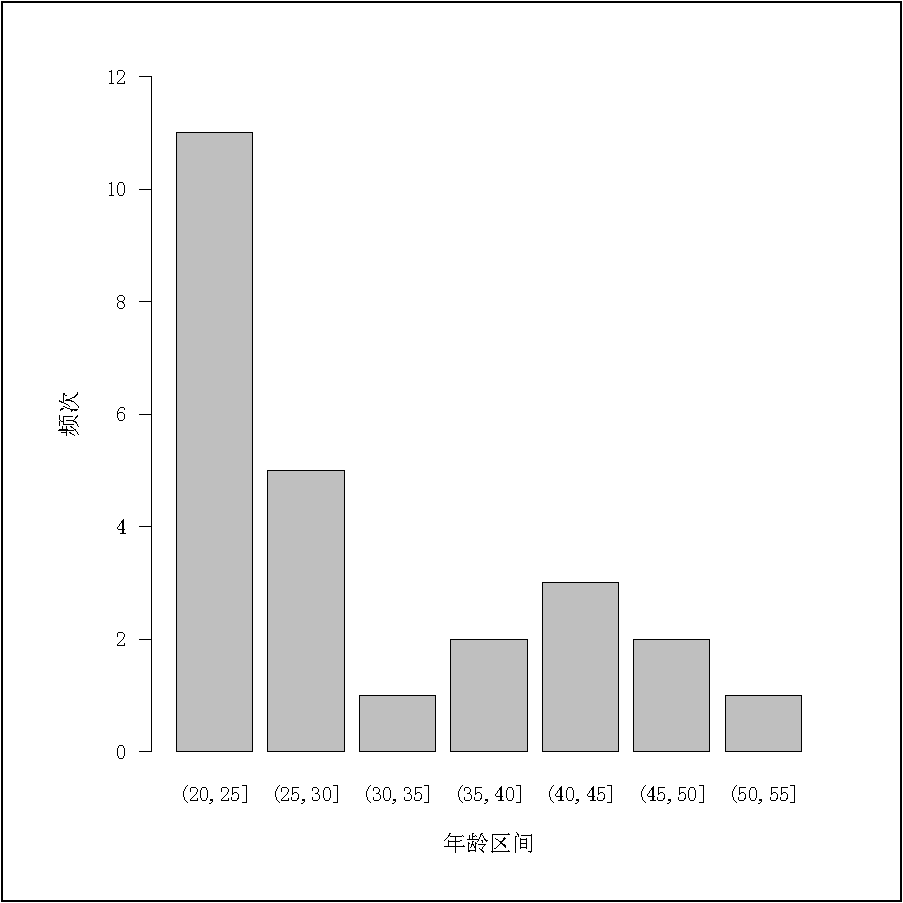
\includegraphics[width=\textwidth]{chapter4-age_barplot}
\caption{年龄分布柱状图}
\label{age_barplot}
\end{minipage}%
\hspace*{0.04\linewidth}
\begin{minipage}[t]{0.48\linewidth}
\centering
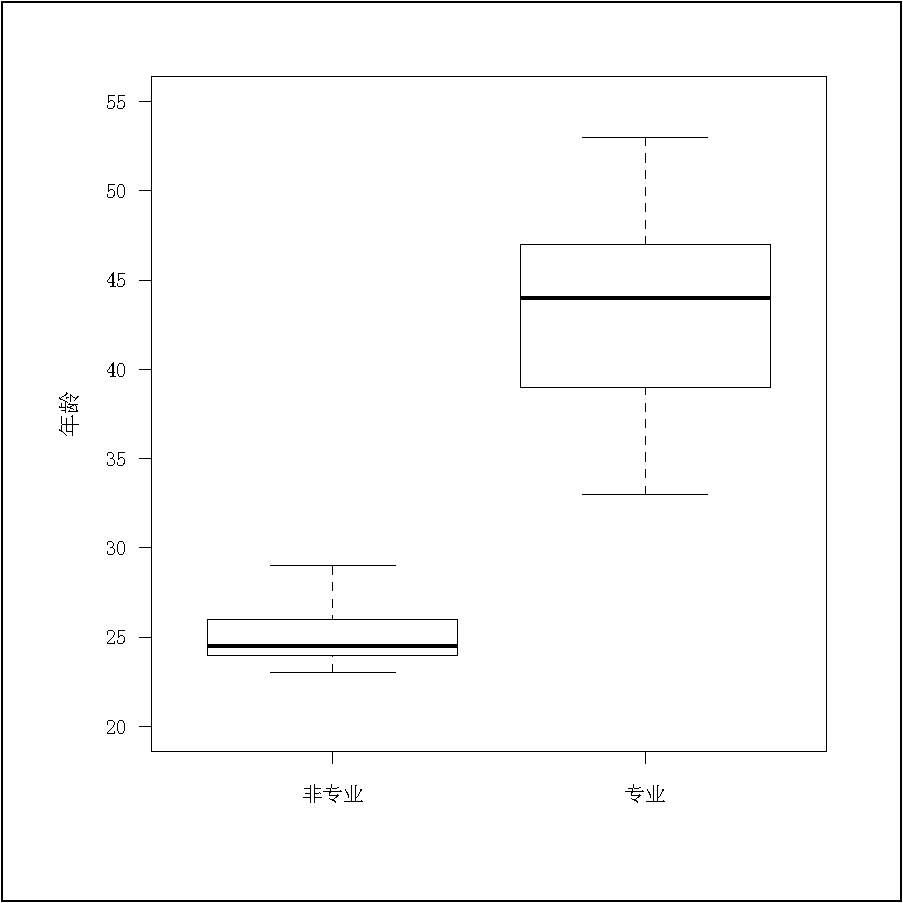
\includegraphics[width=\textwidth]{chapter4-age_boxplot}
\caption{非专业与专业组年龄箱图}
\label{age_boxplot}
\end{minipage}
\end{figure}

\begin{figure}
\begin{minipage}[t]{0.48\linewidth}
\centering
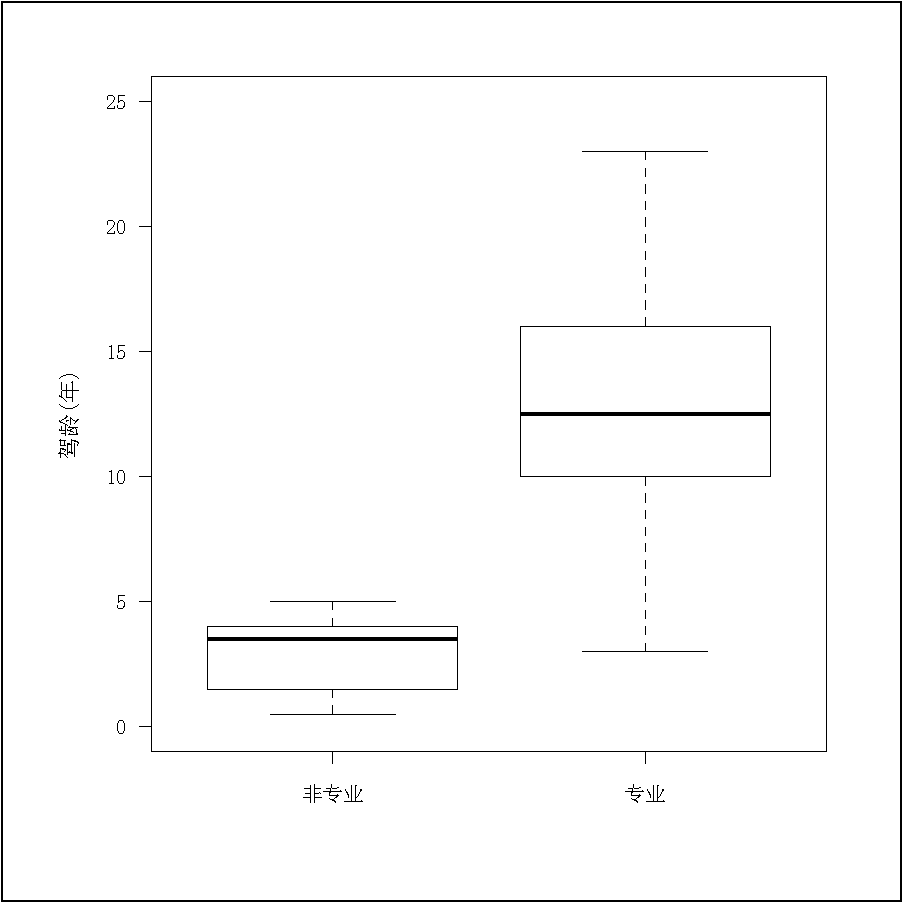
\includegraphics[width=\textwidth]{chapter4-certified_boxplot.pdf}
\caption{非专业与专业组驾龄箱图}
\label{certified_boxplot}
\end{minipage}%
\hspace*{0.04\linewidth}
\begin{minipage}[t]{0.48\linewidth}
\centering
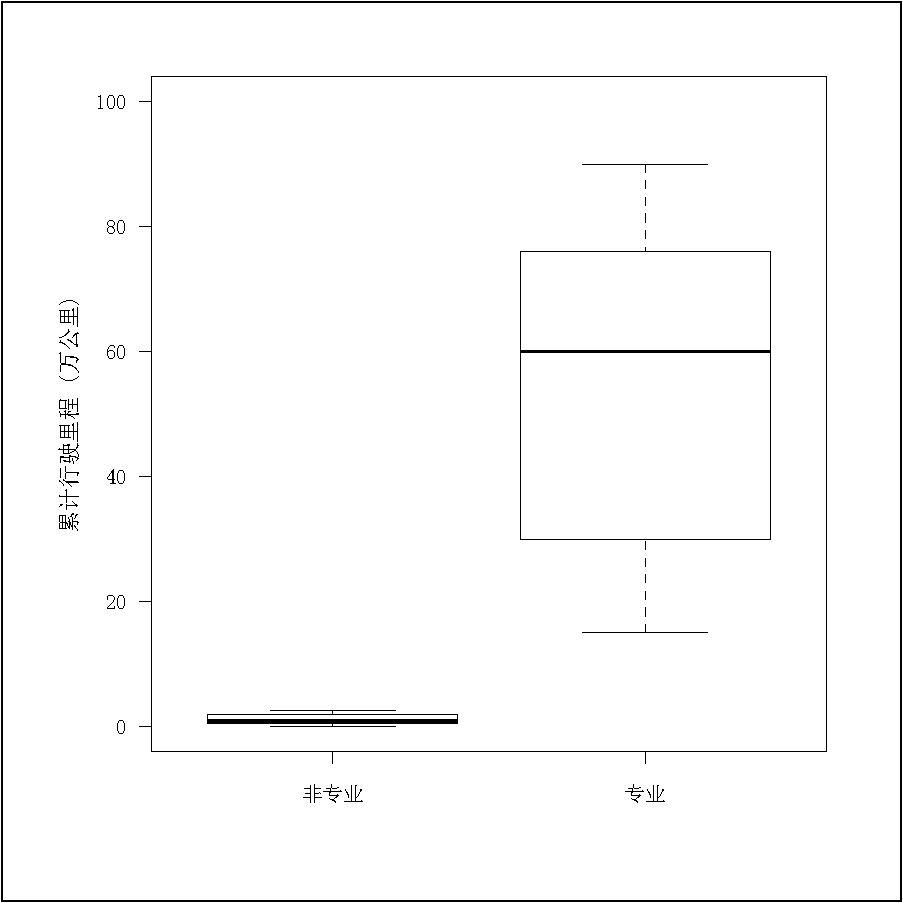
\includegraphics[width=\textwidth]{chapter4-mileage_boxplot.pdf}
\caption{非专业与专业组累计里程箱图}
\label{mileage_boxplot}
\end{minipage}
\end{figure}




\subsubsection{数据的基本情况}

通过实验获取共60041s(约16.6hr)的数据,就单个驾驶人而言最短的数据741s,最长的数据3623s。\autoref{d_density,v_density,acc_density}给出了原始数据中测试车的跟驰距离,速度和加速度分布情况。由于城市路段交通情况的特点,跟驰距离主要集中在20米以内,峰值出现在2-6m之间。车速的分布,由于停车较多,速度为0的分布频次最多,而在0-40km/h的区间内分布比较平均,40-60km/h分布逐渐减少,很少有超过60km/h的车速。实验车加速度的分布峰值出现在0$m/s^2$,分布范围主要在[-2,2]$m/s^2$的区间。总体上数据的基本情况符合实际测试的交通状况。





\begin{figure}[h]
\begin{minipage}[t]{0.48\linewidth}
\centering
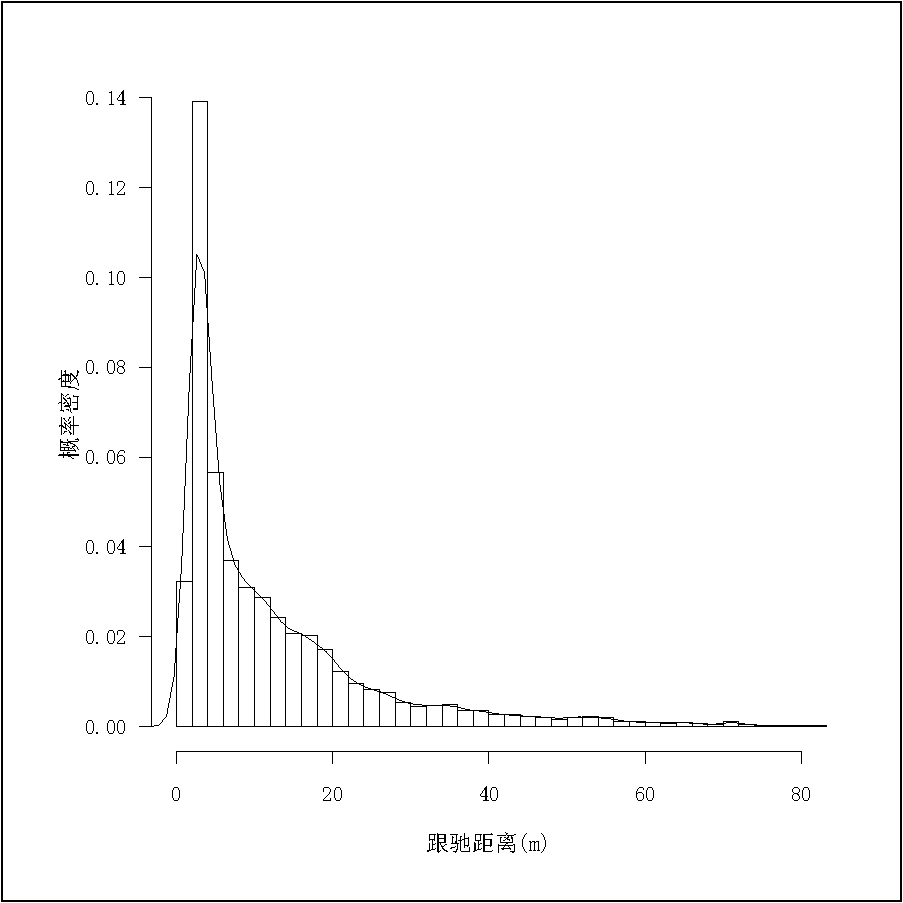
\includegraphics[width=\textwidth]{chapter4-d_density}
\caption{跟驰距离的核密度估计图}
\label{d_density}
\end{minipage}%
\hspace*{0.04\linewidth}
\begin{minipage}[t]{0.48\linewidth}
\centering
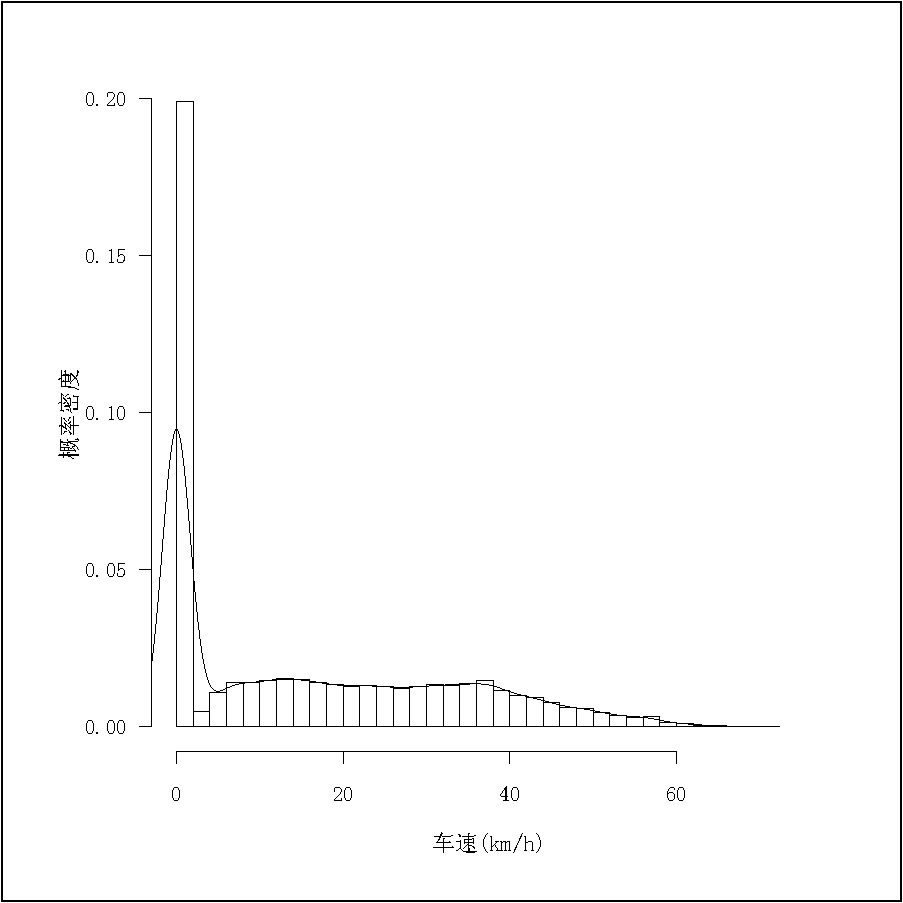
\includegraphics[width=\textwidth]{chapter4-v_density}
\caption{车速的核密度估计图}
\label{v_density}
\end{minipage}
\end{figure}

\begin{figure}[htbp]
\centering
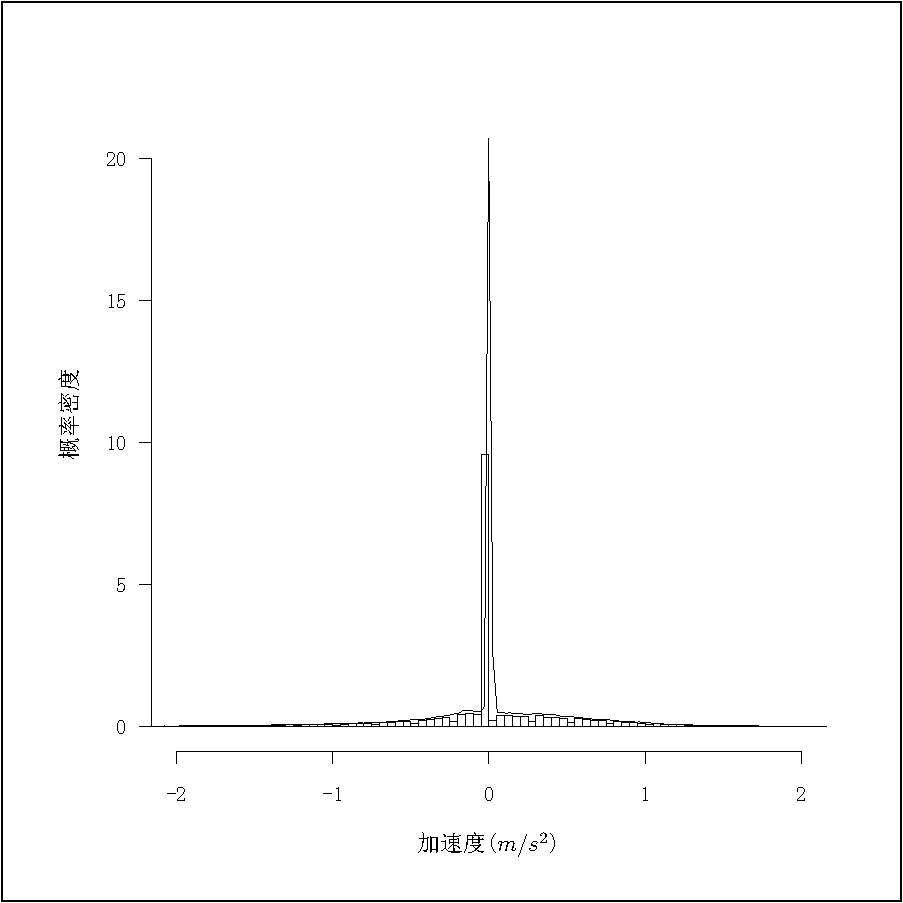
\includegraphics[width=0.48\linewidth]{chapter4-acc_density}
\caption{加速度的核密度估计图}
\label{acc_density}
\end{figure}







\subsection{数据处理}


由于激光测距系统的固有特性,所测的的原始数据中前车轨迹数据主要存在两方面的问题。其一,前车动态的数据不连续。激光测距测速仪安装于实验车上,在行驶过程中,受到前车尾部高度,反射率,车辆转向等因素的影响,其射出的光束并不能保证时刻得到有效的返回光束,因此也无法测出实验车与前车的相对动态关系。其二,所得数据存在随机误差(系统误差已通过试验设备的校准尽可能减小),随机误差理论上应符合正态分布,随机误差将使实验数据的分析发生偏差,Ossen(2008)\cite{Ossen2008}的实验表明,车辆轨迹的测量误差会对驾驶人行为参数的估计产生不可忽略的影响,因此有必要对数据进行后处理。对于车辆轨迹的后处理的最主要目的是得到对于真实轨迹的偏差尽可能小的估计。

目前研究中针对轨迹数据的处理主要有以下几种方法。

1.简单移动平均


最简单的轨迹数据后处理是简单移动平均,Thiemann等\cite{Thiemann2008}使用对称指数移动平均来平滑处理NGSIM的轨迹数据,发现了误差在差分过程中的放大效应,使得误差从位置,速度,加速度放大地向下传递,并使用移动平均来抵消这一效应。移动平均(低通滤波器)通常需要进行敏感性分析来确定移动平均的窗口大小和权重函数,从而使得既能够降低噪声又能保存原有信号中的高频部分。一般通过频谱分析来确定截断频率。

% The most basic filtering technique is the simple moving average. (16) use a 
% symmetric exponential moving average filter to smooth NGSIM data. They detect the magnification of noise 
% after differentiation and address it first by differentiating positions to speeds and accelerations and then by 
% smoothing all three variables. 
% Moving average generally needs a sensitivity analysis to find windows and weights that provide the 
% best tradeoff between the damping of the noise and the losing of high frequency parts of original trajectories. In 
% general, attention must be paid when using such techniques (or low-pass filters) since they may remove some 
% detailed information while leaving part of the noise. Therefore it would advisable if the choice and the design of 
% filters were preceded by spectral analysis of data. Such analysis can give useful information e.g. to decide the 
% most appropriate cut-off frequency and to design the frequency response of the filter. 

2.卡尔曼滤波

Ervin, R.等\cite{Ervin2000}使用卡尔曼滤波的方法对SAVME系统采集的轨迹数据进行了平滑处理,Punzo等\cite{Punzo2009}使用类似的方法对GPS采集的轨迹数据进行了处理。卡尔曼滤波需要对车辆的运行模型进行假设,而研究车辆的运行模型往往是采集轨迹数据的目的,因此若本文使用卡尔曼滤波进行轨迹数据的处理存在逻辑上的矛盾。
% The Kalman filter needs a simple traffic model and
% thus introduces some significant assumptions into the smoothing process. Also, the Kalman
% filter has more parameters while the sEMA method has only one parameter, T, and does not
% introduce complicated assumptions.

% Ervin et al. (6, 7) used Kalman
% filtering to smooth trajectory data collected by using video cameras
% with the SAVME system. Punzo et al. (8) used a similar approach
% with data collected by using GPS technology. The Kalman filter was
% applied with average speeds that were derived from the raw data.
% Thus, the result was smoothed average measurements rather than
% instantaneous ones. Although the difference between the two types
% of measurements may be negligible for the very short time intervals
% (0.1 s) reported in their application, it is expected to be more signif-
% icant for longer intervals. Furthermore, with the SAVME system, the
% Kalman filter is based on a model of the vehicle dynamics. However,
% the development of such model is, in most cases, the purpose of the
% data collection effort.

3.局部加权回归

Toledo等\cite{Toledo2007a}提出了使用局部加权回归的方法对轨迹数据进行处理的方法,局部加权回归可以较好地使用多项式拟合高度非线性的函数,可以用来处理轨迹数据和速度数据。Toledo等\cite{Toledo2007a}的研究表明局部加权回归结果对于参数选择,测量误差和缺失测量值均是较为稳定的。
% The approach uses local regression, a
% method well suited for mapping highly nonlinear functions. The proposed
% methodology is applied to a set of position data. The results demonstrate
% the value of the method to development of vehicle trajectories and speed
% and acceleration profiles. The conducted sensitivity analysis also shows
% that the method is rather robust regarding measurement errors and
% missing values.

本文中根据所测数据的特性,比较各种方法后选取局部加权回归的方法对轨迹数据进行处理,并根据一定的原则通过筛选,获取合理的数据。


%介绍local regression的原理和作用
\subsubsection{局部加权回归}
Cleveland\cite{Cleveland1979}最早提出了局部加权回归的方法,局部加权回归在每一点使用数据的一个子集(一般选取以拟合点中心对称的一个“窗口”)通过低阶的多项式函数进行拟合,多项式系数的估计采用加权最小二乘法,对于靠近拟合点的数据给予较高的权重而远离拟合点的数据则反之,得出拟合函数后计算拟合点的数值。局部加权回归可以灵活的选取窗口大小和权重函数以适应不同的应用需求。
% At each point in the data set a low-degree polynomial is fitted to a subset of the data, with explanatory variable values near the point whose response is being estimated. The polynomial is fitted using weighted least squares, giving more weight to points near the point whose response is being estimated and less weight to points further away. The value of the regression function for the point is then obtained by evaluating the local polynomial using the explanatory variable values for that data point. The LOESS fit is complete after regression function values have been computed for each of the n data points. Many of the details of this method, such as the degree of the polynomial model and the weights, are flexible. The range of choices for each part of the method and typical defaults are briefly discussed next.


对前车数据应用局部加权回归时,需要进行3个参数的选择,分别是权重函数,多项式次数和窗口大小。

根据实际情况,本文处理中权重函数选取了Tricube核函数,
\begin{equation}
w(t_0,t)=(1-u(t_0,t)^3)^3
\end{equation}

\begin{equation}
u(t_0,t)=\frac{\left | t-t_0 \right |}{d}
\end{equation}

其中:
\begin{displaymath}
{\begin{aligned}
w(t_0,t)&=\text{中点为}t_0\text{时}t\text{点的权重}\\
u(t_0,t)&=t\text{到}t_0\text{的规格化距离}\\
d&=t_0\text{到窗口外最近一点的距离}\\
\end{aligned}}
\end{displaymath}



其形状如\autoref{tricub}

\begin{figure}[htbp]
\begin{minipage}[t]{0.48\linewidth}
\centering
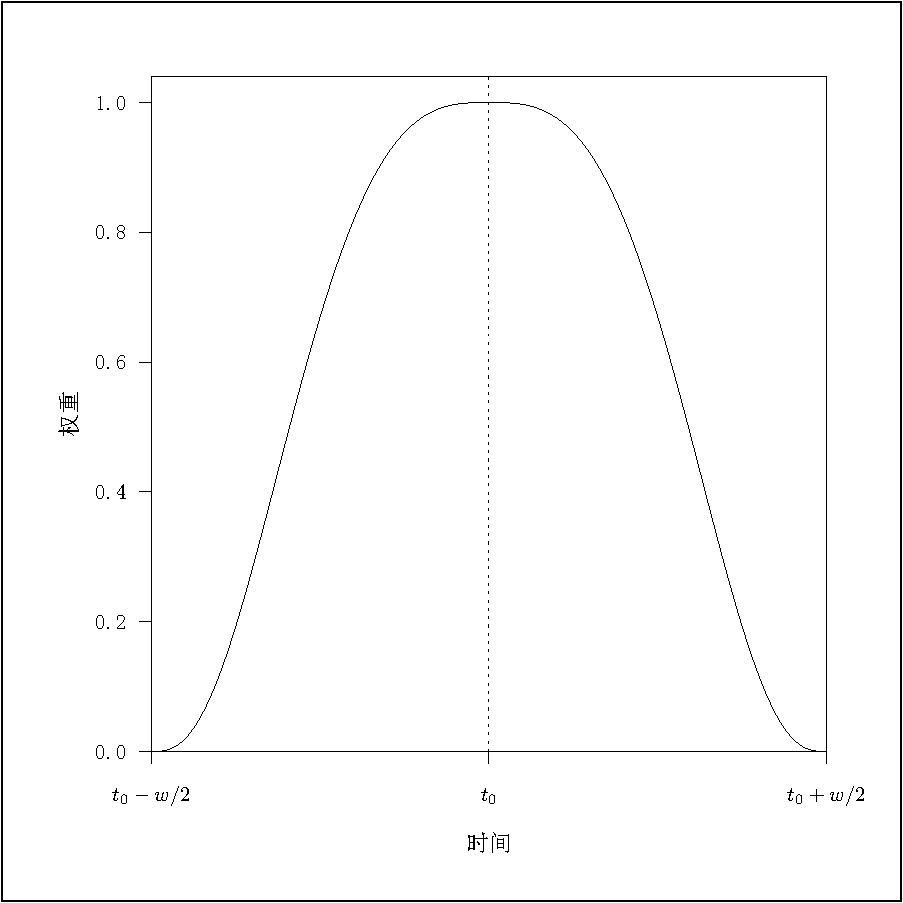
\includegraphics[width=\textwidth]{chapter4-tricub}
\caption{Tricube核函数示意图}
\label{tricub}
\end{minipage}%
\hspace*{0.04\linewidth}
\begin{minipage}[t]{0.48\linewidth}
\centering
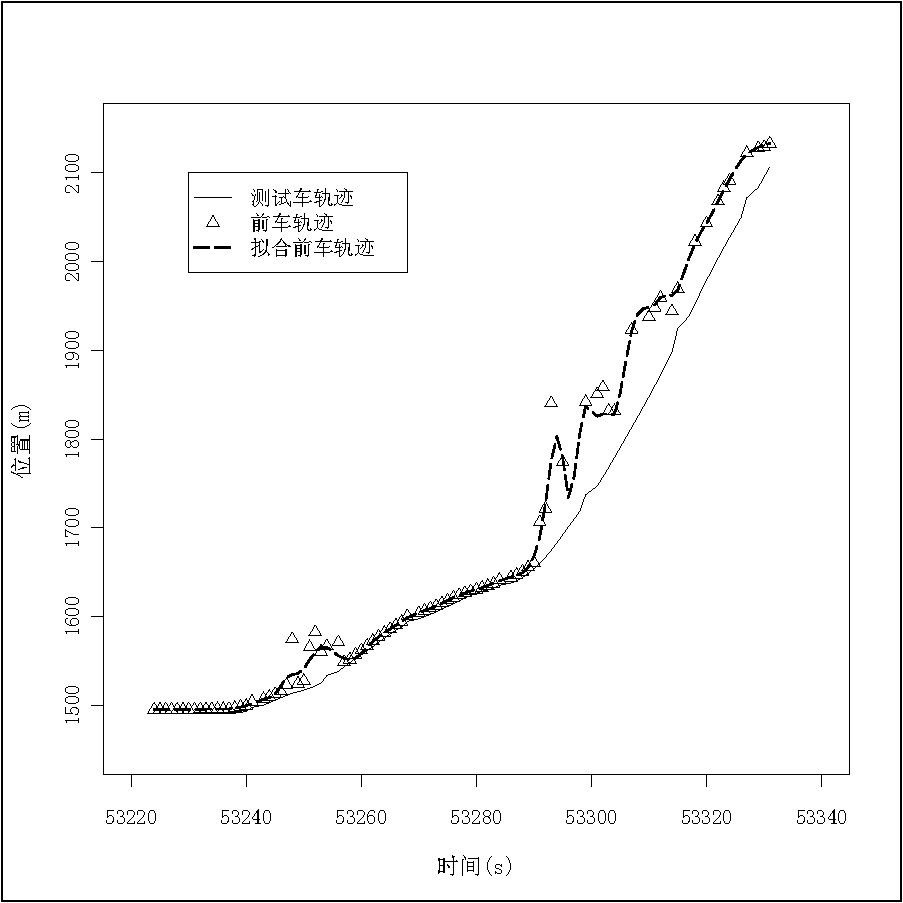
\includegraphics[width=\textwidth]{chapter4-sample-processing}
\caption{前车(引导车)轨迹数据局部回归示意图}
\label{sample-processing}
\end{minipage}
\end{figure}


为了保证回归后所得数据的合理性,需要保证回归多项式次数至少为3次,从而当从轨迹数据求导获取速度和加速度数据时,速度和加速度不会退化为常数。而过高的次数会增加计算的复杂度,并且高次多项式需要更大的数据窗口进行拟合,因此本文中选取多项式次数为3,窗口大小选择为11个数据点,一般会覆盖到1s的时间。


经过局部回归处理后的数据,还需要对数据进行筛选,合理的前车轨迹数据应符合以下两个条件,其一由于正常行驶中车辆不后退,因此轨迹数据应为非严格单调增函数;其二由于车辆运动的宏观连续性,拟合数据与原始数据较大的差值往往表明原始数据中前车运动已经超过可能的物理极限,为无效数据,因此有效的局部回归数据应与原始数据较为吻合。其三前车数据应符合交通情况和物理极限,例如车速超过60km/h和加速度在[-5,10]$m/s^2$之外的应为无效数据。


\autoref{sample-processing}为对前车轨迹数据处理的样例,例如图中53260s到53290s的数据为回归拟合较好的数据,而53300s周围的数据由于出现车辆倒退为无效数据,需要排除在有效数据之外。


\subsubsection{处理结果}
\label{process-result}
%start from here 2011
经过数据处理与数据筛选后,60041s的数据中共24374s大约40.6\%的数据成为最终用于分析的数据。经过处理后的数据中实验车数据的跟驰距离,车速和加速度分布如\autoref{postprocess-d-density,postprocess-v-density,postprocess-acc-density}


\begin{figure}[htbp]
\begin{minipage}[t]{0.48\linewidth}
\centering
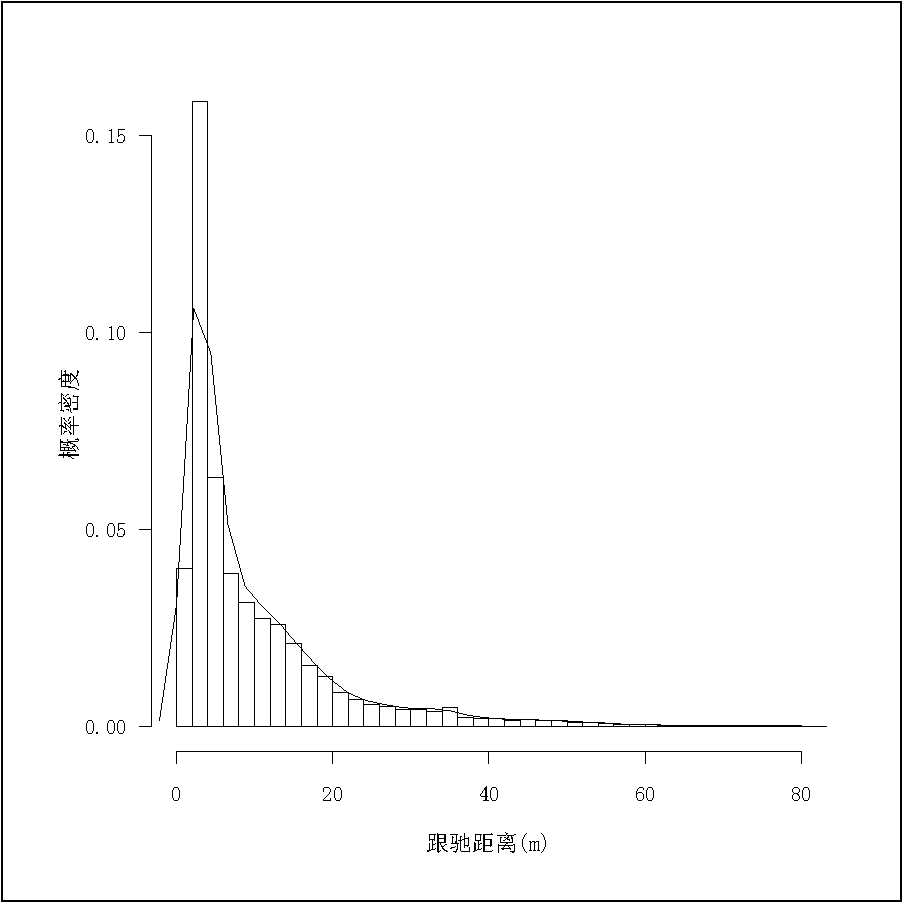
\includegraphics[width=\textwidth]{chapter4-postprocess-d-density}
\caption{处理后跟驰距离概率核密度估计图}
\label{postprocess-d-density}
\end{minipage}%
\hspace*{0.04\linewidth}
\begin{minipage}[t]{0.48\linewidth}
\centering
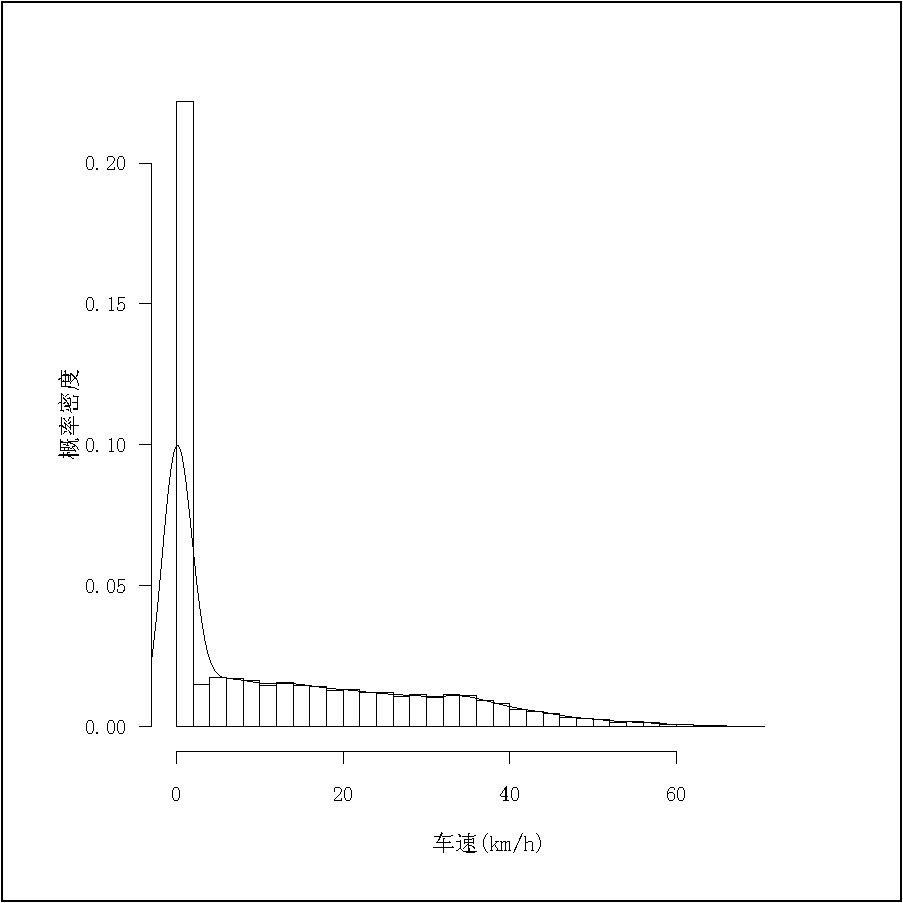
\includegraphics[width=\textwidth]{chapter4-postprocess-v-density}
\caption{处理后速度概率核密度估计图}
\label{postprocess-v-density}
\end{minipage}
\end{figure}

\begin{figure}[htbp]
\centering
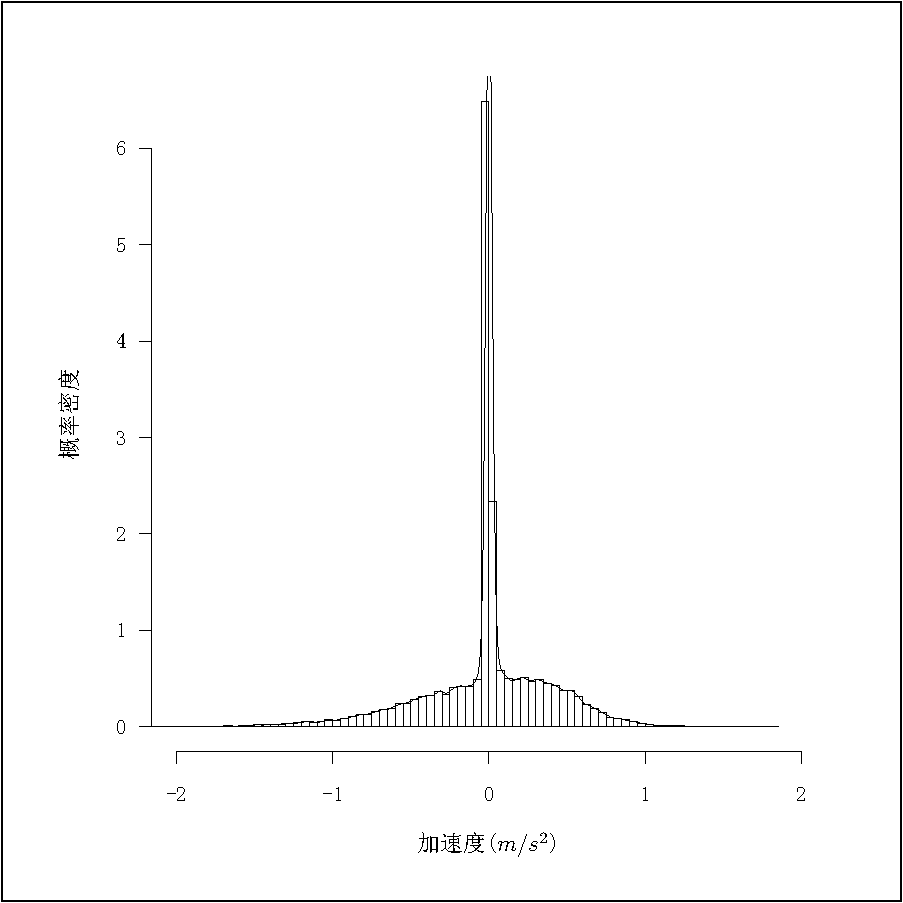
\includegraphics[width=0.48\linewidth]{chapter4-postprocess-acc-density}
\caption{处理后加速度概率核密度估计图}
\label{postprocess-acc-density}
\end{figure}


处理后的数据参数分布,其形状对比\autoref{d_density,v_density,acc_density},可以看出数据处理并未对数据的固有特征造成显著的影响,因此可以认为数据处理未对原始数据进行有偏差的抽取。

%\section{问卷信息}
\section{跟驰行为特性的集计分析}
本节通过对数据的集计,对专业与非专业驾驶人的行为特性进行初步的分析,从而研究专业与非专业驾驶人驾驶行为的异同。分析主要针对三个方面,一,自由流与跟驰的临界点;二,稳定状态下跟驰距离与速度的关系;三,加速度与车辆相互运动的关系。

\subsection{自由行驶与跟驰的临界点}
% Discerning free driving from car-following state plays an essential role in modeling driver’s car-following behavior. Many car following models distinguish free driving from car following state, and assume that a driver tends to drive at a desired speed until getting influenced by vehicles ahead of him. It is also conceivable that the influence of frontal vehicle is larger for short time/space distance and smaller for longer time/space distance. But how distant away a driver starts to engage frontal vehicle and get into car-following state has not been fully studied. 

车辆的行驶可认为存在自由行使和跟驰两种状态,自由行驶是指车辆在不受前车影响下的自由行驶。而跟驰情况下,车辆速度受到前车速度的影响。一般可以假设认为,前车对于驾驶人的影响大小与其时间或空间意义上的距离有关,距离越小则影响越大而距离越大则影响越小。自由行驶和跟驰的临界点是影响跟驰行为的重要因素,因此也是反映驾驶人行为特性的一个指标。

% Based on the obtained data the method proposed by K. Vogel was used to determine the threshold between free driving and car following. The reasoning of the scheme is briefly described as follows.
% The criterion for separating ‘‘free’’ and following vehicles is that the speed of a free vehicle should not be influenced by the speed of the vehicle ahead. Thus, the speeds of the two vehicles should not correlate.
Vogel(2002)\cite{Vogel2002}提出了通过定点测量的车头时距和车速数据确定自由行驶与跟驰的临界点的方法,根据车头时距和车头间距对数据进行分组,其后计算每组数据内前后车速度的相关系数来代表前车对后车速度的影响程度。其数据表明当车头时距大于一定数值后,车速的相关系数出现突然的下降,通过假设临界点分别对假设的跟驰数据和自由行使数据进行线性拟合试算,当两组数据的拟合的交点与分割点最为接近时则认为得到了自由行驶与跟驰的临界点。

本文中针对所获取的数据,基于Vogel的方法,使用时间间隔替换车头时距分别对专业和非专业驾驶人的数据进行了自由行驶与跟驰的临界点的确定。
对于所有的数据,将时间间隔数据舍入到最近的秒数,例如时间间隔在0.5至1.5秒坐开右闭区间的归入到1秒的组别,在1.5至2.5秒坐开右闭区间的归入到2秒的组别,依此类推。对于超过20.5秒的数据由于数据量很少不能得到可靠的速度相关系数值,因此排除在考察数据之外。

对专业和非专业驾驶人,分别计算速度相关系数,并进行线性回归的试算,其结果如\autoref{tab-free-discern},回归示意图如\autoref{nonpro-tgap-discern,pro-tgap-discern}。

\begin{table}[htbp]
  \centering
  \caption{自由行驶与跟驰临界点结果表}
    \begin{tabular}{ccc}
    \addlinespace
    \toprule
          & 专业驾驶人 & 非专业驾驶人 \\
    \midrule
    临界点时间间隔 & 6.5s  & 11.5s \\
    跟驰拟合R平方 & 0.9899 & 0.9925 \\
    自由行驶拟合R平方 & 0.3302 & 0.0892 \\
    交点 & 6.06s & 11.34s \\
    跟驰拟合方程 & y=-0.06526x+ 0.93158 & y=-0.0679x+ 0.9996 \\
    自由行驶拟合方程 & y=-0.02613x+ 0.69439 & y=-0.00752x+ 0.31514 \\
    \bottomrule
    \end{tabular}%
  \label{tgap-discern}%
\label{tab-free-discern}
\end{table}%

\begin{figure}[htbp]
\begin{minipage}[t]{0.48\linewidth}
\centering
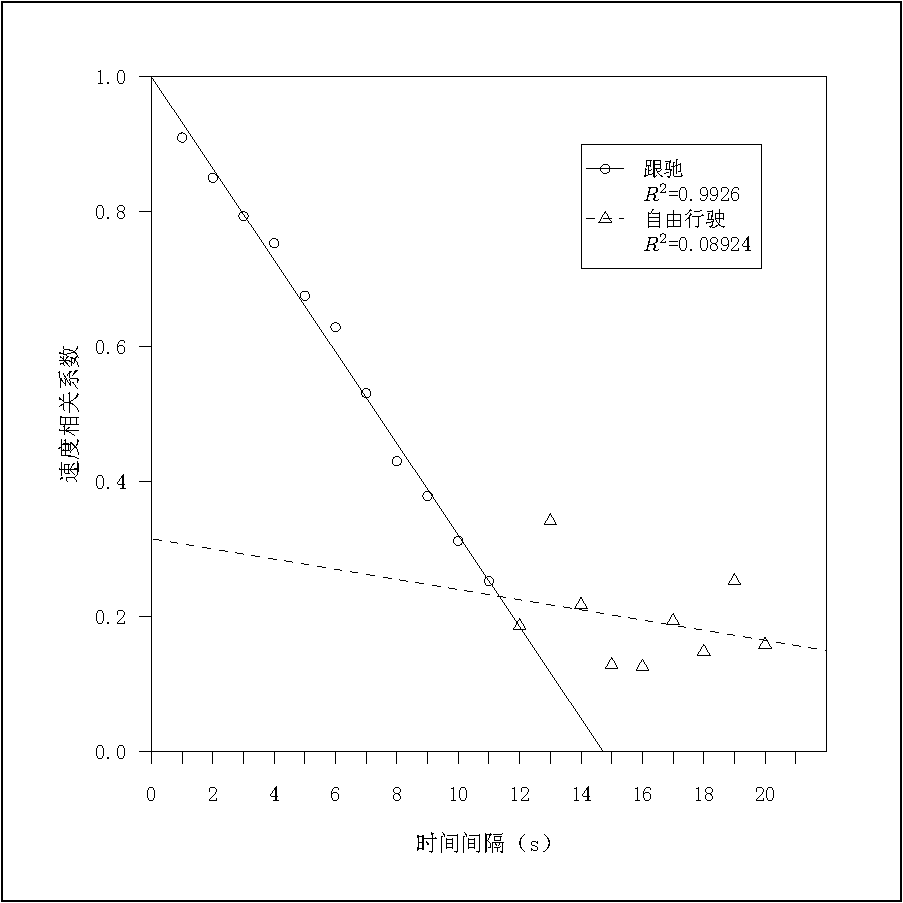
\includegraphics[width=\textwidth]{chapter4-nonpro-tgap-discern}
\caption{非专业驾驶人时间间隔-速度相关系数图}
\label{nonpro-tgap-discern}
\end{minipage}%
\hspace*{0.04\linewidth}
\begin{minipage}[t]{0.48\linewidth}
\centering
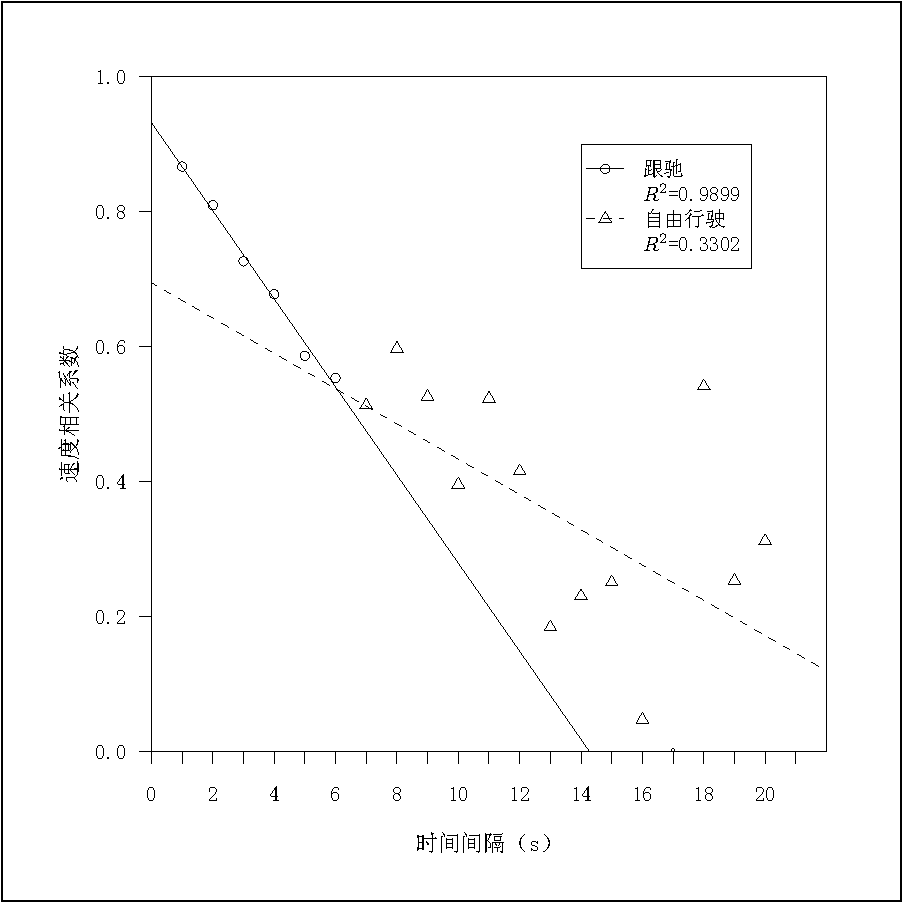
\includegraphics[width=\textwidth]{chapter4-pro-tgap-discern}
\caption{专业驾驶人时间间隔-速度相关系数图}
\label{pro-tgap-discern}
\end{minipage}
\end{figure}





% Upon this approach, the criterion for determining the cut-off point for free and following vehicles would be the x-axis value of the intercept point of the two regression lines. It should be as close as possible to the time/space distance value which was used to split the data into the two subgroups. If this were not the case, it would indicate that the division was not made at the correct location. The empirical data would need to yield a drop in correlation values at the threshold. Therefore it is basically the task to find regression lines that intersect close to the split point to get the threshold.

% For all observations the time gap was rounded to the nearest second, and then grouped according to time gap. For example, vehicles with time gaps between 0.5 s (excluded) and 1.5 s (included) fell into group 1 with a rounded time gap of 1 s, vehicles with a time gap between 1.5 (excluded) and 2.5 s (included) fell into group 2 with a rounded time gap of 2 s, and so on. Vehicles with time gaps that are longer than 20.5 s were too scarce to provide reliable estimate of speed correlation and are excluded. 

% For the two drivers’ groups, in each time gap interval the speed correlation was calculated. The correlation values of the two drivers’ group are plotted in Fig and Fig; for each driver’s group the speed correlations all decreased while time gaps increased. However, they show quite different patterns. 
% For the experienced group with a time gap of 1 s the correlation value was about r=0.9, i.e. more than 80% of the variance in speed was explained by the speed of the vehicle ahead. For each additional second in time gap, up to 6 s, the correlation value r decreased substantially. For time gaps of more than 6 s and less than 12 s the correlation values started to fluctuate but still decreased in trend, and the slope was not as steep as before 6 s. For time gaps of more than 12 s the speed correlation went under 0.4.

% For beginners group with a time gap of 1s the correlation value was also about r=0.9. For each additional second in time gap, up to 12s, the correlation value r decreased substantially, for time gaps of more than 12s the curves appear to level out. For headways of 12s and longer, the speed of frontal vehicle accounted for no more than 10% of the speed of subject vehicle.
结果显示,对于专业驾驶人1s的时间间隔其速度相关系数为0.9,也就是说超过80\%的泵车速度变化可以由前车的速度解释,到6s之前每增加1s的时间间隔,速度相关系数均显著下降。在6s与12s之间速度相关系数产生一些波动,总体上仍呈现下降趋势。超过12s后速度相关系数减小到0.4以下;对于非专业驾驶人,1s的时间间隔其速度相关系数也约为0.9,直到12s速度相关系数均显著下降,超过12s后速度相关系数减小到0.1以下。
% Based on these observations, for each driver group possible split points were chosen. One linear regression was computed on the correlation values below the split point; another linear regression was computed above the split point. The best split point turned out to be 6.5 s and 11.5 s for experienced and beginner group respectively. Results are provided in Table 1, regressions are shown in Figure. 5 and Figure. 6 
从专业与非专业自由行驶与跟驰临界点结果看,专业驾驶人的临界点为6.5s,非专业驾驶人为11.5s,这似乎意味着非专业更早的受到前车的影响而进入跟驰的状态,但是结合速度相关系数的数值,在(6.5,11.5]的时间间隔区间内,专业驾驶人的速度相关系数要大于非专业驾驶人的相应数值。将(6.5,11.5]的时间间隔区间内的数据选出,得到专业驾驶人8159组数据,非专业驾驶人7245组数据,计算前后车辆的速度差值,两组数据基本上呈正态分布。分别统计得到专业驾驶人速度差中位数为0.3281m/s,标准差4.357m/s;非专业驾驶人速度差中位数为0.3677m/s,标准差4.801m/s。通过Levene检验,专业组与非专业组的速度差方差存在统计意义的显著差别(P<0.01)。以上结果表明在(6.5,11.5]的时间间隔区间内,驾驶人仍然有与前车保持速度一致的趋势,同时专业驾驶人的速度差分散程度要小于非专业驾驶人。综合所得结果可以推断,对于专业和非专业驾驶人在一定的时间间隔内,均受到前车速度影响,相比于非专业驾驶人专业驾驶人似乎能更好地将自身的车速与前车保持一致,尤其是在稍大的时间间隔区间,因此可以认为专业驾驶人有更为“平滑”的驾驶特性。
%The results presented above suggest a 6.5s time gap separation between free driving and car following for the experienced group and accordingly 11.5s for the beginners group. It would seem that beginner drivers start to engage leading vehicle earlier in the time gap sense than experienced drivers. However, the results needs careful interpretation. Although the separation point for the experienced group is 5s longer than that of the beginners group, the speed correlation for the experienced group was generally larger in between the (6.5,11.5] time gap section. For both group the speed correlation dropped almost linearly as time gap increase before the separation point. Before the separation point, time gap all explained over 90% variance of speed correlation. But above the separation point, time gap only accounted for less than 10% of the speed correlation variance for beginners group, yet accounted for 33% of the speed correlation variance for experienced group. Based on the findings,  it is possible to surmise drivers do not differ in perceiving influence from frontal vehicle but differ in taking action. Thus it would be reasonable to choose 12s time gap to be a separation point between free driving and car-following.
% The 12s time gap value is greater than the former proposed 6s time headway value reported by K. Vogel. This clearly suggests the separation point between free driving and car-following is not universal. The variation could come from different sources, e.g. the different road and traffic conditions, different driving behaviors and certainly the different technology used to measure the behavioral data. In order to account for this variation , further investigation is needed and should focus on the influence of different road and traffic conditions.
%In addition, the patterns showed in Figs indicate a difference between the two driver groups. Further analysis was done to explore the difference between driver groups. Data in the (6.5, 11.5] time gap section was picked out for both groups. The experienced group consisted of 8159 observations and the beginners group consisted of 7245 observations. The speed difference (speed of leading vehicle minus speed of subject vehicle) of each observation was calculated for both groups. Central tendency of speed differences was given by the median value: 0.3677m/s for beginners and 0.3281m/s for experienced drivers and sample standard deviations were 4.801 and 4.357 respectively. The low median values suggest drivers tend to adapt their speed to frontal vehicle in the (6.5, 11.5] time gap section. Levene’s test was performed to check the equality of variances. The result showed the speed difference variance of the two groups differed significantly (P<0.01). This combined with the S.D. values indicate experienced drivers adapt his speed to frontal vehicle better.


\subsection{稳定状态下跟驰距离与速度的关系}
%speed-distance profile
速度-跟驰距离选择反应了驾驶人跟驰行为特性中相对稳定的部分,驾驶人根据出行计划,道路条件,交通流条件来选择车速,当车辆的加速度小于一定的阈值时则认为处于稳定的跟驰状态,此时驾驶人根据其选择的车速会与引导车保持一定的跟驰距离。

基于稳定状态下跟驰距离与速度有关的假设,将实验中所获取的数据加速度绝对值小于0.1$m/s^2$的数据选出并分组集计:分别对专业组和非专业组驾驶人按照速度分组,计算每组相应的平均跟驰距离和平均速度,其关系如\autoref{stable-v-distance}。

由\autoref{stable-v-distance}可以看出,整体上跟驰距离随车速的增加而增加,这符合一般认识。对平均车速和平均跟驰距离进行线性回归,得到回归方程。对于专业驾驶人$d_1(m)=1.557 v_1(m/s) + 3.8652$,其$R^2=0.3277$。对于非专业驾驶人$d_2(m)=1.830 v_2(m/s) + 2.6901$,其$R^2=0.4466$

\begin{figure}[htbp]
\begin{center}
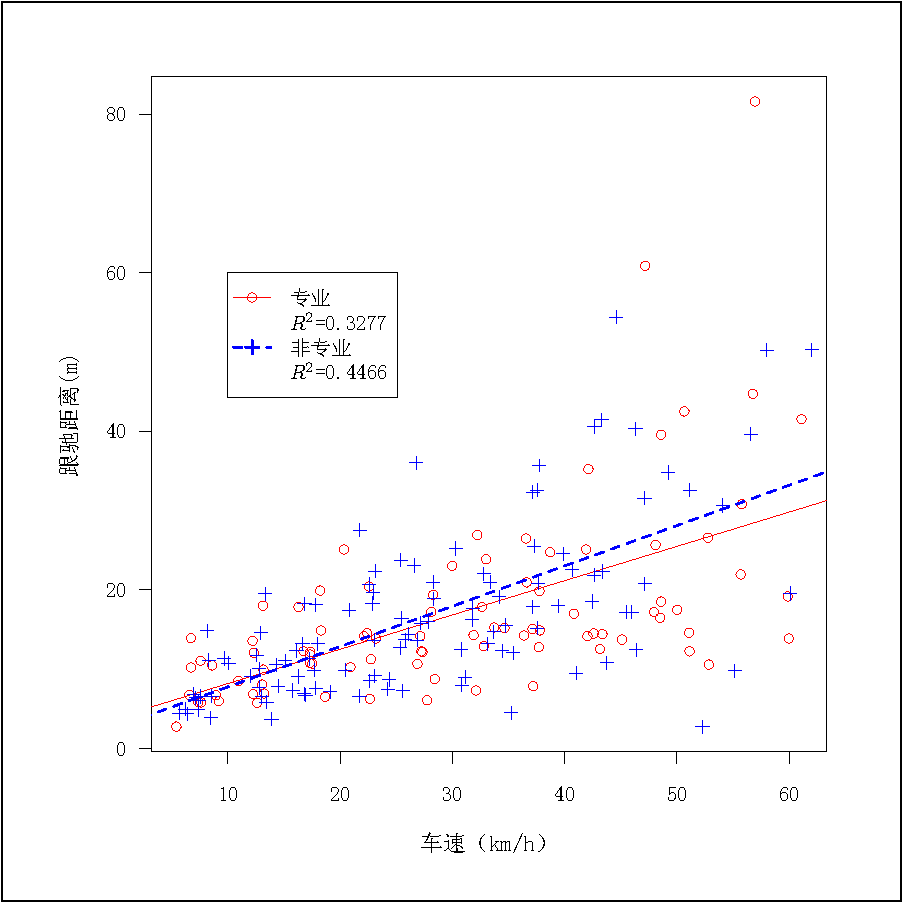
\includegraphics[width=0.6\linewidth]{chapter4-stable-v-distance}
\end{center}
\caption{稳定状态下跟驰距离与速度关系图}
\label{stable-v-distance}
\end{figure}

通过设置虚变量可以检验(T检验)专业组和非专业组的回归系数的差异是否显著。设置虚变量$PRO$,对专业驾驶人$PRO=1$,非专业驾驶人$PRO=0$,则通过回归:
\begin{equation}
d=h_1 \cdot PRO+h_2\cdot v + h_3 \cdot PRO \cdot v +b
\end{equation}
其中$h_1$为截距差,$h_3$为斜率差。

得到\autoref{h-b-df},结果表明两组线性回归的斜率与截距均无统计意义的显著差异(P=0.05水平下,不能拒绝$h_1=0$或$h_3=0$的假设)。因此此处集计分析的证据,不能支持专业与非专业驾驶人的稳定状态下跟驰距离与速度关系特性存在显著差异的观点。

\begin{table}[htbp]
\label{h-b-df}
\begin{center}
\caption{专业组和非专业组的跟驰距离与速度关系回归系数的差异显著性检验}
\begin{tabular}{rrrrr}
  \addlinespace
  \toprule
 & 估计值 & 标准误差 & t值 & P值 \\ 
  \midrule
b & 2.69 & 1.83 & 1.47 & 0.14 \\ 
  $h_1$ & 1.18 & 2.77 & 0.42 & 0.67 \\ 
  $h_2$ & 1.83 & 0.21 & 8.75 & 0.00 \\ 
  $h_3$ & -0.27 & 0.30 & -0.90 & 0.37 \\ 
   \bottomrule
\end{tabular}
\end{center}
\end{table}


\subsection{加速度与车辆相互运动的关系}
%acceleration-speed-difference profile
加速度与车辆相互运动的关系反应了驾驶人跟驰行为特性中相对不稳定的部分。按照刺激反应模型的假设,驾驶人在一定的相对速度下选择相应的合适的加速度,当与前车有接近趋势时则选择负的加速度,有远离趋势时选择正的加速度,而驾驶人采取的加速度与受到的刺激(速度差)成正比。一般化的GM模型认为加速度不仅与速度差有关还与跟驰距离以及车速有关。


Xin等(2008)\cite{Xin2008}提出了驾驶人加速度模型,认为驾驶人的与前车的视觉扩张率有关,但是未明确指出其关系。其视觉扩张率指,物体投射在视网膜上的角度的变化率,
\begin{equation}
tan(\frac{\theta}{2})=\frac{W/2}{D(t)}
\end{equation}

\begin{equation}
\frac{sin(\theta)}{\dot{\theta}}=\frac{D(t)}{\Delta V}
\end{equation}
其中:



\begin{displaymath}
{\begin{aligned}
\theta&=\text{前车投射在视网膜上的角度}\\
\dot{\theta}&=\text{前车投射在视网膜上的角度的变化率即视觉扩张率}\\
W&=\text{前车宽度}\\
D(t)&=t\text{时刻的车头间距}\\
\Delta V&=\text{相对速度}\\
\end{aligned}}
\end{displaymath}


在驾驶过程中前车投射在驾驶人视网膜上的角度较小,因此视觉扩张率可以近似为:
\begin{equation}
\theta \approx \frac{W}{D}
\end{equation}


\begin{equation}
\frac{\theta}{\dot{\theta}}=\frac{D(t)}{\Delta V}
\end{equation}

\begin{equation}
\dot{\theta}=W\frac{\Delta V}{D^2}
\end{equation}

在交通冲突技术中Time-To-Collision(TTC)被证明是有效的度量交通冲突严重程度的手段。Hayward(1972)\cite{Hayward1972}定义TTC为;“两车保持当前速度和路线而相撞所需要的时间。”Lee(1976)\cite{Lee1976}定义TTC为两物体距离比上其相对速度。Balas和Balas(2006)\cite{Balas2006}比较了TTC倒数和TTC,认为TTC倒数比TTC更为直接和连续的反映了碰撞的危险,并且认为TTC倒数可用于解释驾驶人的驾驶行为。

基于加速度与速度差跟驰距离有关的观点,假设前车宽度基本不变,将实验中所获取的数据分组集计:分别对专业组和非专业组驾驶人按照速度差距离比$\frac{\Delta V}{D}$即TTC倒数,加速度与速度差距离平方比$\frac{\Delta V}{D^2}$进行分组,计算每组相应的平均速度差距离比,平均速度差距离平方比,以及平均加速度,得到关系如\autoref{a-deltavbyd,a-deltavbyd2}。

\begin{figure}[htbp]
\begin{minipage}[t]{0.48\linewidth}
\centering
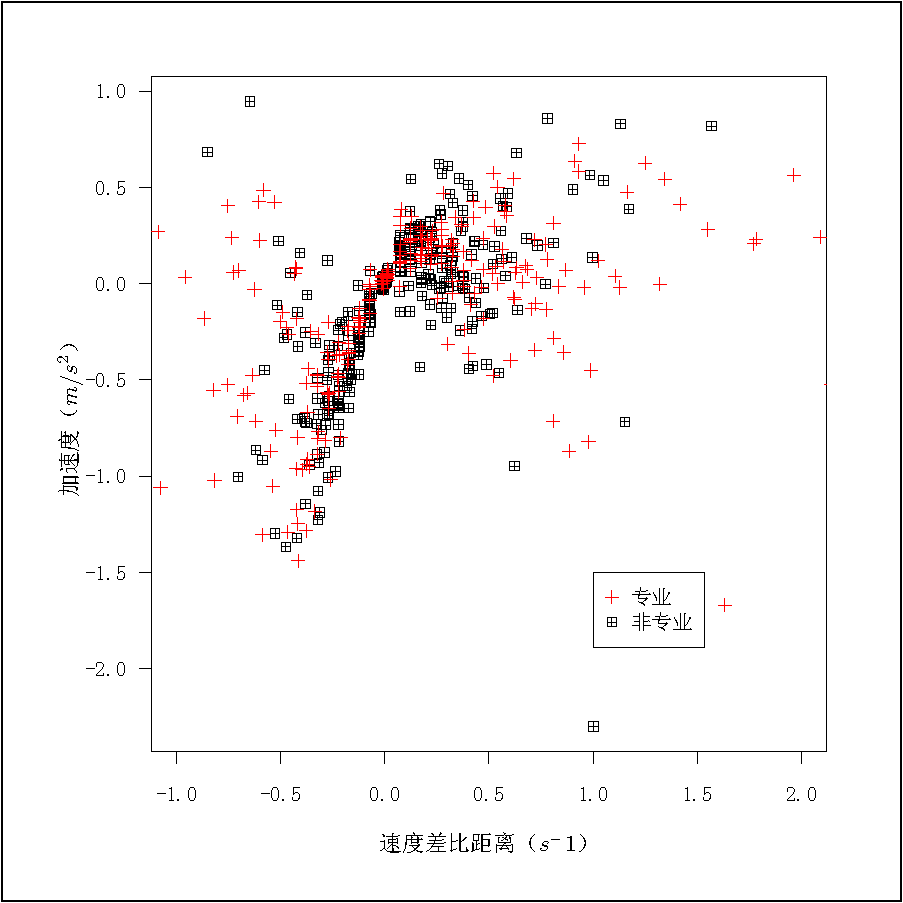
\includegraphics[width=\textwidth]{chapter4-a-deltavbyd}
\caption{加速度与速度差距离比图}
\label{a-deltavbyd}
\end{minipage}%
\hspace*{0.04\linewidth}
\begin{minipage}[t]{0.48\linewidth}
\centering
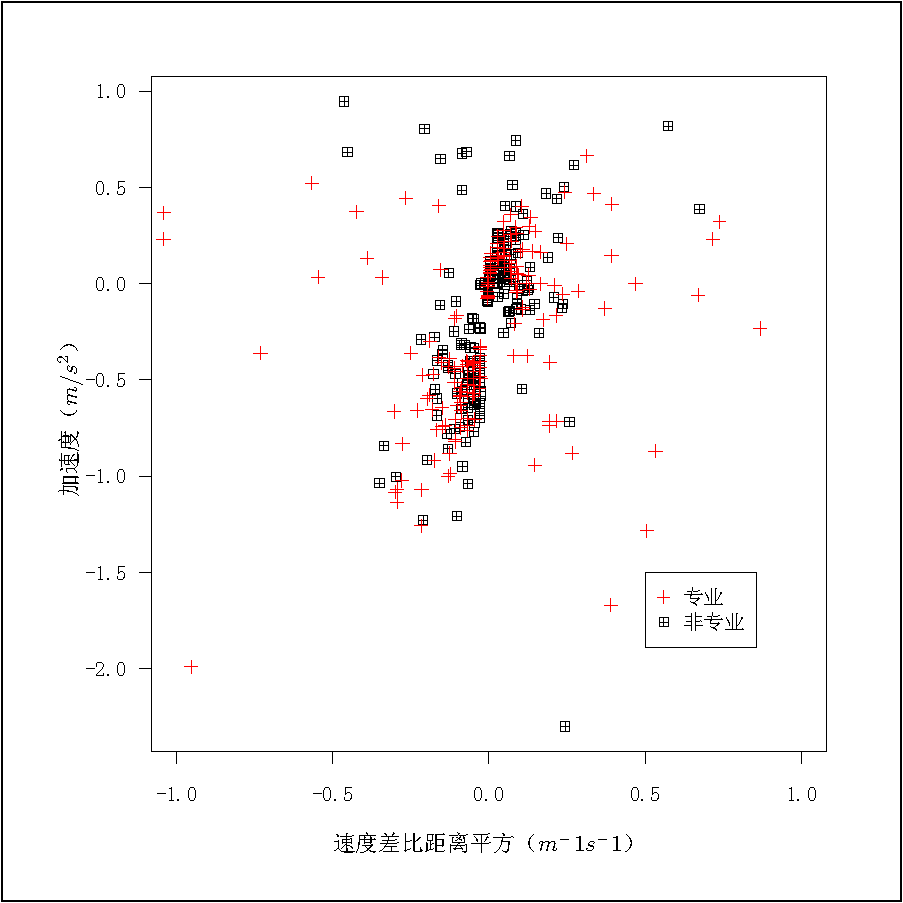
\includegraphics[width=\textwidth]{chapter4-a-deltavbyd2}
\caption{加速度与速度差距离平方比图}
\label{a-deltavbyd2}
\end{minipage}
\end{figure}


对于前车速度小于跟驰车辆的情况,由\autoref{a-deltavbyd,a-deltavbyd2}中的速度差轴左侧可以发现速度差距离比(TTC倒数)与驾驶人的负减速度存在明显的线性关系,说明驾驶人对于减速情况减速度的选择与速度差距离比有较大的相关性。而加速度与速度差距离平方比的线性关系则较不明显。而当速度差为正时驾驶人的加速度的分布均十分的分散,这表明驾驶人减速与加速之间存在不对称性。同时专业组和非专业组之间并未表现出明显的差别。


\subsection{集计分析小节}
从集计分析的结果可以发现专业和非专业驾驶人驾驶行为特性的差异得到了混合的结果,在自由行驶与跟驰的临界点方面存在明显的差别,而在稳定状态下速度与跟驰距离,加速度与车辆相互运动的关系特性方面不存在明显的差别。

%一方面可能是样本的代表性问题,专业组和非专业组的差别除了驾驶经验以外还有年龄和职业等的差异,因此专业组与非专业组的区别并不是一个单纯的影响因子。

由于集计分析忽略了更多驾驶条件的影响,例如在相同的速度差条件下速度值不同采取的加速度可能也不同。由于集计对驾驶人不同驾驶条件下的数据进行了平均,因此还需要对数据进行进一步的分析。下一节中将从更加微观的角度分析,使用跟驰模型参数标定的方法,分析跟驰模型参数在驾驶人中的分布情况,并作出相应的分析和推断。



%因此不能排除驾驶人在组内的差异性,

%同时结果表明驾驶人自身在加速与减速过程存在显著的差异性。






\section{跟驰模型参数标定}
为了进一步研究驾驶人行为特性的异同,并且为通过模拟研究驾驶人行为特性对交通流影响提供依据,本节使用轨迹数据对微观跟驰模型参数进行标定,并使用Bootstrap方法对所得结果进行分析和推断。
\subsection{标定方法框架}
Ossen(2008)\cite{Ossen2008}给出了一般化的通过轨迹数据标定跟驰模型的框架:

以$z_n(t)$表示驾驶人n车辆的真实行驶状态,此状态一般包含车辆的位置$x_n(t)$与速度$v_n(t)$,以$\xi_n(t)$表示驾驶人n所面临的交通条件,向量$\xi_n(t)$包含驾驶人n对于前方若干辆车的位置、速度等变量的观察和估计:

\begin{equation}
\xi_n(t)=(z_{n-j}(t),\cdots z_{n-1}(t))
\end{equation}

j为驾驶人n向前观测的车辆个数,本文数据由于技术原因只能测到向前一辆车的动态,标定中也将使用单引导车模型,因此:
\begin{equation}
\xi_n(t)=z_{n-1}(t)
\end{equation}

驾驶人车辆纵向的运动可以用跟驰模型来描述则:
\begin{equation}
\frac{d}{dt}z_n(t)=f(\xi_n(t-T_r\mid\beta_n))
\end{equation}

则系统的变化方程为:
\begin{equation}
\hat{z}_n(t_k)=\left\{\begin{matrix}
y_n(t_1))& k=1\\
\hat{z}_n(t_{k-1})+\int_{t_{k-1}}^{t_k} f(\xi_n(s-T_r)\mid\hat{\beta}_n)ds& \text{其他}
\end{matrix}\right.
\end{equation}

标定的目标就是找到最优的参数$\beta^*_n$使得目标函数最小:
\begin{equation}
\beta^*_n=argmin_{\hat{\beta}_n}g(y_n,\hat{z_n})
\end{equation}

其中g为目标函数,数量化度量模型预测结果和真实结果的差别。

\subsection{跟驰模型}

跟驰模型选用IDM(Intelligent Driver Model)智能驾驶模型,IDM模型自提出以后由于其优良的特性被广泛研究,IDM模型参数较少且具有明确易理解的物理意义。IDM模型统一描述了自由行驶和跟驰,并且可以体现加速和减速的不对称性。



Treiber等(2000)\cite{Treiber2000}和Treiber和Helbing(2003)\cite{Treiber2003}假设加速度受到期望速度和期望跟驰距离的影响提出了IDM模型,Kesting和Treiber(2008)\cite{Kesting2008}对其参数进行了标定。其形式如下:
% assume that the acceleration is
%affected by both the desired speed and the desired minimum space headway. The
%model also incorporates the impact of vehicle capabilities, but ignores reaction
%time: 
\begin{equation}
a_n(t)=a_{max}\left[1-\left(\frac{V_n(t)}{DV_n(t)}\right)^4-\left(\frac{D_n(t)}{\Delta X_n(t)}\right )^2\right],
\end{equation}
其中$a_{max}$为车辆的最大舒适加速度。$V_n$为实际车速,$DV$为期望速度,$D_n$为期望跟驰距离,$\Delta X_n$为实际跟驰距离。

%其期望车头间距给出如下:
%
%\begin{equation}
%D_n(t)=\Delta X_n^*+V_n(t)T_n(t)+\frac{V_n(t)\Delta V_n(t)}{2\sqrt{a_{max}b_{max}}},
%\end{equation}

驾驶人车辆的加速度由两个部分组成,其趋向自由行驶部分的加速度为:
\begin{equation}
a_{max}\left[1-\left(\frac{V_n(t)}{DV_n(t)}\right)^4\right],
\end{equation}

受前车影响部分的加速度为:
\begin{equation}
-a_{max}\left[\left(\frac{D_n(t)}{\Delta X_n(t)}\right )^2\right],
\end{equation}
当实际的跟驰距离小于期望跟驰距离时,此项成为加速度的主要部分。

其期望车头间距给出如下:
\begin{equation}
D_n(t)=\Delta X_n^*+V_n(t)T_n(t)+\frac{V_n(t)\Delta V_n(t)}{2\sqrt{a_{max}b_{max}}},
\end{equation}
其中$\Delta X_n^*$为停车间距,$T_n$为期望车头时距,当距离较小时$\Delta X_n^*$占期望跟驰距离的主要部分,$T_n$期望车头时距体现了驾驶人对安全跟驰距离的一种期望。$b_{max}$为最大舒适减速度。在大多数情况下将减速度的绝对值限制在其以下。






\subsection{目标函数}

g为目标函数,数量化度量模型预测结果和真实结果的差别。本文中使用Theil's U作为目标函数,
\begin{equation}
g(y_n,\hat{z}_n)=\frac{\sqrt{\frac{1}{K} \sum\limits_{k=1}^{K}(y_n(t_k)-\hat{z}_n(t_k))^2}}{\sqrt{\frac{1}{K} \sum\limits_{k=1}^{K}(y_n(t_k))^2}+\sqrt{\frac{1}{K} \sum\limits_{k=1}^{K}(\hat{z}_n(t_k))^2}}
\end{equation}
其中$y_n$为实际观测值,$\hat{z}_n$为模型预测值,考虑到本文数据采集所使用的方法以及交通流状况,使用跟驰距离而不考虑将速度代入到$y_n$和$\hat{z}_n$中计算,理由是实验数据中直接测量的变量包括跟驰距离,而前车速度经过计算得出,误差经由一次求导会被放大。城市交通流状况存在较多的停车,以速度代入也将使目标函数对参数过于敏感不利于得到合理的标定值。

\subsection{优化算法与搜索范围}
本文使用遗传算法(genetic algorithm)对目标函数进行优化,遗传算法是计算数学中用于解决最优化的搜索算法,是进化算法的一种。进化算法最初是借鉴了进化生物学中的一些现象而发展起来的,这些现象包括遗传、突变、自然选择以及杂交等。

遗传算法通常实现方式为一种计算机模拟。对于一个最优化问题,一定数量的候选解(称为个体)的抽象表示(称为染色体)的种群向更好的解进化。一般解用二进制表示(即0和1的串)。进化从完全随机个体的种群开始,初代种群产生之后,按照适者生存和优胜劣汰的原理,逐代(generation)演化产生出越来越好的近似解,在每一代,根据问题域中个体的适应度(fitness)大小选择(selection)个体,并借助于自然遗传学的遗传算子(genetic operators)进行组合交叉(crossover)和变异(mutation),产生出代表新的解集的种群。这个过程将导致种群像自然进化一样的后生代种群比前代更加适应于环境,末代种群中的最优个体经过解码(decoding),可以作为问题近似最优解。


本文的参数优化过程使用了Walter等\cite{WRMebane2009}开发的Rgenoud解法器,初始种群个数设为1000,目标函数无改进阈值设置为0.001,无改进停止代数10代。本文中共需标定5个参数,分别是$DV$期望车速,最大舒适加速度$a_{max}$,最大舒适减速度$b_{max}$,期望车头时距$T$,最小间距$\Delta X^*$。设置参数的搜索范围可以减少运算量并可保证所得结果在合理的范围内,参数的搜索范围如\autoref{param_range}。


% Table generated by Excel2LaTeX from sheet 'Sheet1'
\begin{table}[htbp]
  \centering
  \caption{参数标定搜索范围}
    \begin{tabular}{rrrrrr}
    \addlinespace
    \toprule
    参数    & $DV(m/s)$    & $a_{max}(m/s^2)$    & $b_{max}(m/s^2)$    &  $\Delta X^*(m)$    & $T(s)$ \\
    \midrule
    范围    & [0,30] & [0.3,3] & [0.5,10] & [0,5] & [0,5] \\
    \bottomrule
    \end{tabular}%
  \label{param_range}%
\end{table}%


\subsection{轨迹数据与标定结果}
\refsec{process-result}提到经过数据处理大约40.6\%的数据为有效数据,由于测量系统的特性,数据并不连续。为保证轨迹数据含有足够的信息量从而保证参数标定的可靠性,本文选取长度不小于10s的轨迹数据用于参数标定。

结果表明参数标定可以得到拟合良好的轨迹,\autoref{sample-calib-d,sample-calib-v}为标定结果样例,图中可以看到跟驰距离和车速的模型预测值与实际值吻合良好。

结果样例如\autoref{sample-calib-table}。

\begin{figure}[htbp]
\begin{minipage}[t]{0.48\linewidth}
\centering
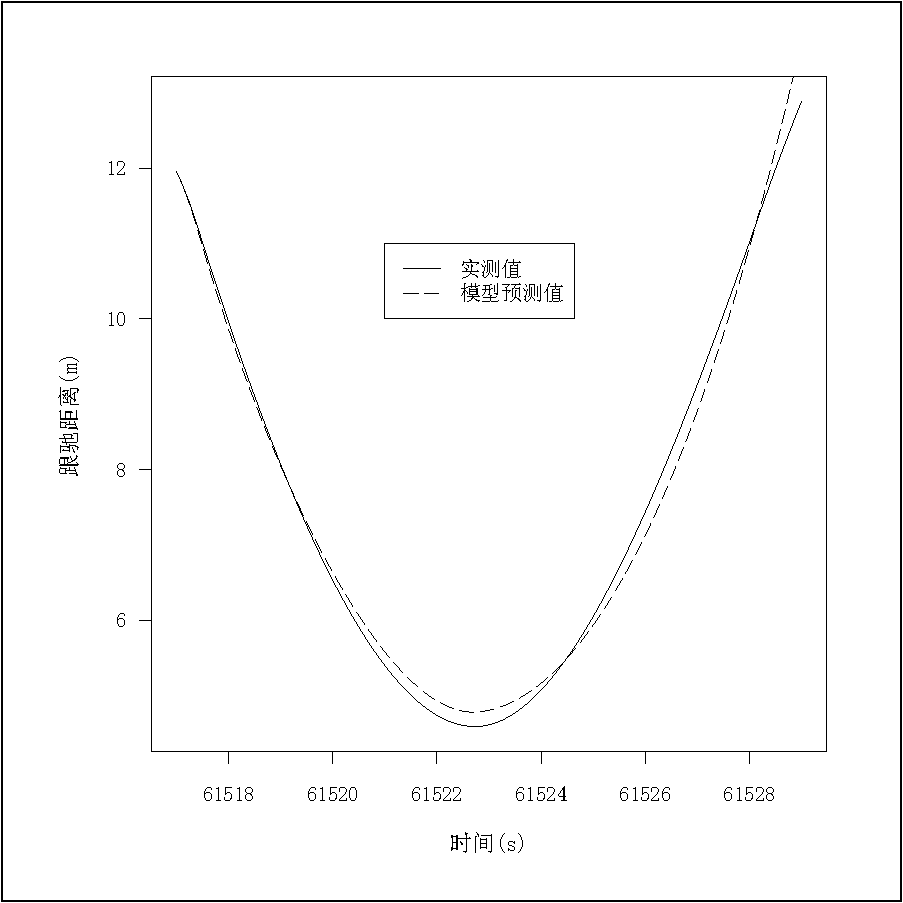
\includegraphics[width=\textwidth]{chapter4-sample-calib-d}
\caption{参数标定结果样例-跟驰距离变化图}
\label{sample-calib-d}
\end{minipage}%
\hspace*{0.04\linewidth}
\begin{minipage}[t]{0.48\linewidth}
\centering
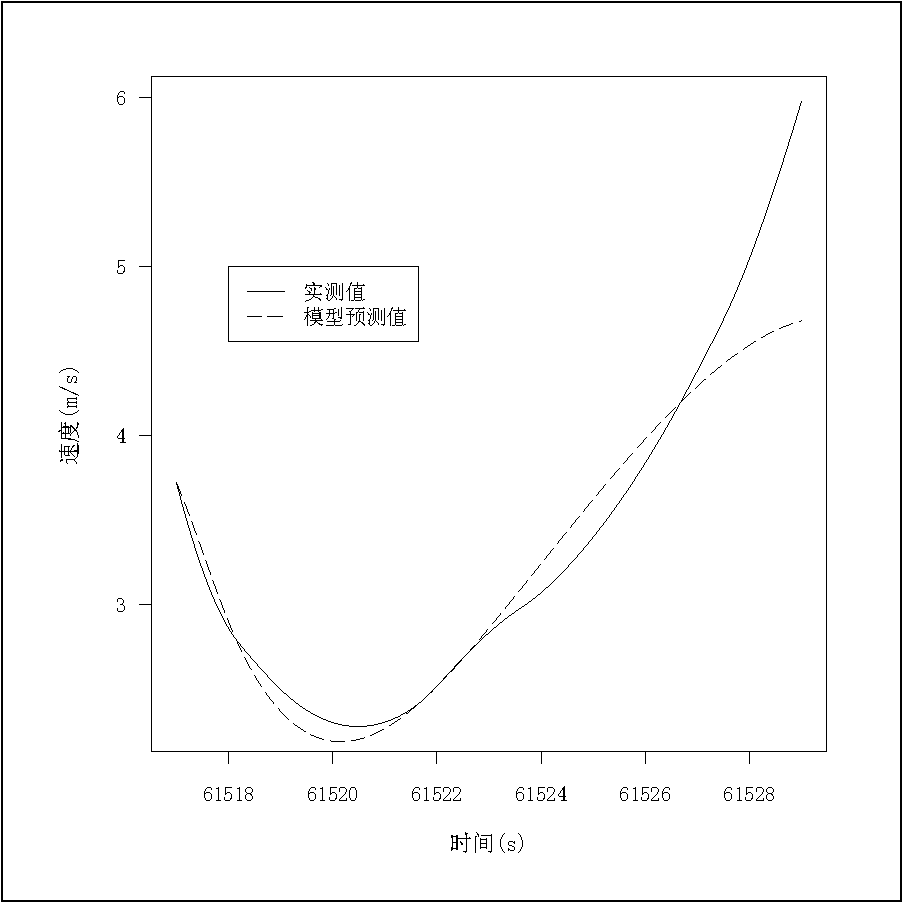
\includegraphics[width=\textwidth]{chapter4-sample-calib-v}
\caption{参数标定结果样例-车速变化图}
\label{sample-calib-v}
\end{minipage}
\end{figure}

% Table generated by Excel2LaTeX from sheet 'calib_result'
\begin{table}[htbp]
  \centering
  \caption{标定参数结果样例}
    \begin{tabular}{rrrrrr}
    \addlinespace
    \toprule
    $DV(m/s)$    & $a_{max}(m/s^2)$    & $b_{max}(m/s^2)$    &  $\Delta X^*(m)$    & $T(s)$ & 目标函数值 \\
    \midrule
    19.10  & 0.62  & 3.42  & 1.20  & 3.90  & 0.02  \\
    9.95  & 0.30  & 0.68  & 4.42  & 4.70  & 0.20  \\
    12.62  & 0.54  & 0.50  & 4.60  & 4.54  & 0.18  \\
    14.00  & 2.88  & 1.00  & 4.80  & 3.99  & 0.46  \\
    1.95  & 0.30  & 5.97  & 1.61  & 4.36  & 0.02  \\
    5.24  & 0.37  & 7.91  & 3.86  & 4.26  & 0.46  \\
    6.28  & 0.63  & 0.53  & 3.44  & 0.84  & 0.13  \\
    2.94  & 2.88  & 0.50  & 4.11  & 3.50  & 0.37  \\
    8.06  & 0.42  & 0.50  & 3.19  & 2.02  & 0.18  \\
    4.19  & 2.04  & 1.80  & 2.37  & 3.15  & 0.23  \\
    21.00  & 0.87  & 9.01  & 0.30  & 3.64  & 0.12  \\
    ...  & ...  & ... & ...  & ...  & ...  \\
    \bottomrule
    \end{tabular}%
  \label{sample-calib-table}%
\end{table}%

%% Table generated by Excel2LaTeX from sheet 'calib_result'
%\begin{table}[htbp]
%  \centering
%  \caption{Add caption}
%    \begin{tabular}{rrrrrrr}
%    \addlinespace
%    \toprule
%    序号    & 参数1   & 参数2   & 参数3   & 参数4   & 参数5   & 目标函数值 \\
%    \midrule
%    1     & 0.0760  & 0.7399  & 6.0596  & 4.9949  & 19.9735  & 0.0523  \\
%    2     & 1.2352  & 0.4298  & 0.5000  & 2.7482  & 5.5988  & 0.0302  \\
%    3     & 1.4037  & 0.5716  & 0.7723  & 2.8879  & 15.5550  & 0.1082  \\
%    4     & 1.9631  & 0.7525  & 2.5320  & 3.1079  & 13.1612  & 0.1056  \\
%    5     & 2.3227  & 0.9399  & 0.5108  & 3.7085  & 8.8214  & 0.1297  \\
%    6     & 13.8583  & 0.3000  & 0.5003  & 0.5603  & 20.0000  & 0.3148  \\
%    7     & 16.9795  & 0.3000  & 0.5000  & 0.6026  & 20.0000  & 0.3120  \\
%    8     & 13.3178  & 0.3067  & 0.5000  & 3.6540  & 6.9455  & 0.7914  \\
%    9     & 1.1541  & 0.4485  & 9.3143  & 2.4454  & 17.8628  & 0.1342  \\
%    10    & 29.4136  & 0.3000  & 0.5000  & 0.3814  & 20.0000  & 0.8865  \\
%    11    & 1.2205  & 0.3000  & 0.5006  & 1.9076  & 17.7410  & 0.4417  \\
%    12    & 14.0335  & 0.3000  & 0.5002  & 0.4269  & 20.0000  & 0.2779  \\
%    13    & 0.0086  & 0.3187  & 8.2771  & 1.8356  & 2.3186  & 0.0137  \\
%    14    & 13.9797  & 0.3000  & 0.5000  & 0.9117  & 20.0000  & 0.5047  \\
%    15    & 14.8697  & 0.3000  & 0.5002  & 0.7457  & 20.0000  & 0.3022  \\
%    16    & 11.6980  & 2.0517  & 1.0119  & 1.8404  & 3.0476  & 0.1829  \\
%    17    & 2.1580  & 0.3000  & 9.0604  & 4.9944  & 19.9765  & 0.1471  \\
%    ...    & ... & ... & ...  & ...  & ...  & ... \\
%    \bottomrule
%    \end{tabular}%
%  \label{tab:addlabel}%
%\end{table}%





\subsection{所得估计参数的可靠程度}

由于车辆轨迹包含的信息不同,因此一段轨迹只能可靠的估计若干个参数,例如一段停车的轨迹是不可能准确地估计出期望车速,最大舒适加速度和最大舒适减速度的参数,却可能很好地估计出停车间距的参数。而加速过程的轨迹则很难估计最大舒适减速度的参数,反之亦然。所以需要估计所得参数的可靠程度。Greene(2000)\cite{Greene2000}指出对于一个变量的点估计其方差至少不小于Cramer-Rao下限,并且指出其值可用对数似然函数在最大似然估计点的二次偏导数估计。Ossen(2008)\cite{Ossen2008}据此提出了使用参数估计点的目标函数二次偏导数来估计参数估计的可靠程度,即:

%二次偏导数与m中位数,variance的关系
\begin{equation}
\left.\frac{\partial^2 g(y_n,\hat{z}_n)}{\partial\beta_i^2}\right| _{\beta_i=\beta_i^*}
\end{equation}

可以理解二次偏导数为估计参数的敏感度,若二次偏导数越大,则不论向任何一个方向一个小的扰动均会造成目标函数值g越大的增加,也就代表参数估计越可靠。

由于所估计参数的取值范围不同,为了统一比较各参数的可靠程度,需对各参数除以其中位数进行规格化,然后计算其二次偏导数。






\subsection{Bootstrap与置信区间估计}
为了得到两组各参数有效的估计,本文中选取目标函数g值0.2以下,并且参数二次偏导数不小于20(则规格化参数改变0.1,目标函数的改变量应在$20\times 0.1^2=0.2$的数量级)的参数估计作为最后的结果进行分析。最终,各参数估计值的分布情况如\autoref{weighted-distr-np1,weighted-distr-pp1,weighted-distr-np2,weighted-distr-pp2,weighted-distr-np3,weighted-distr-pp3,weighted-distr-np4,weighted-distr-pp4,weighted-distr-np5,weighted-distr-pp5,}


\begin{figure}[htbp]
\begin{minipage}[t]{0.48\linewidth}
\centering
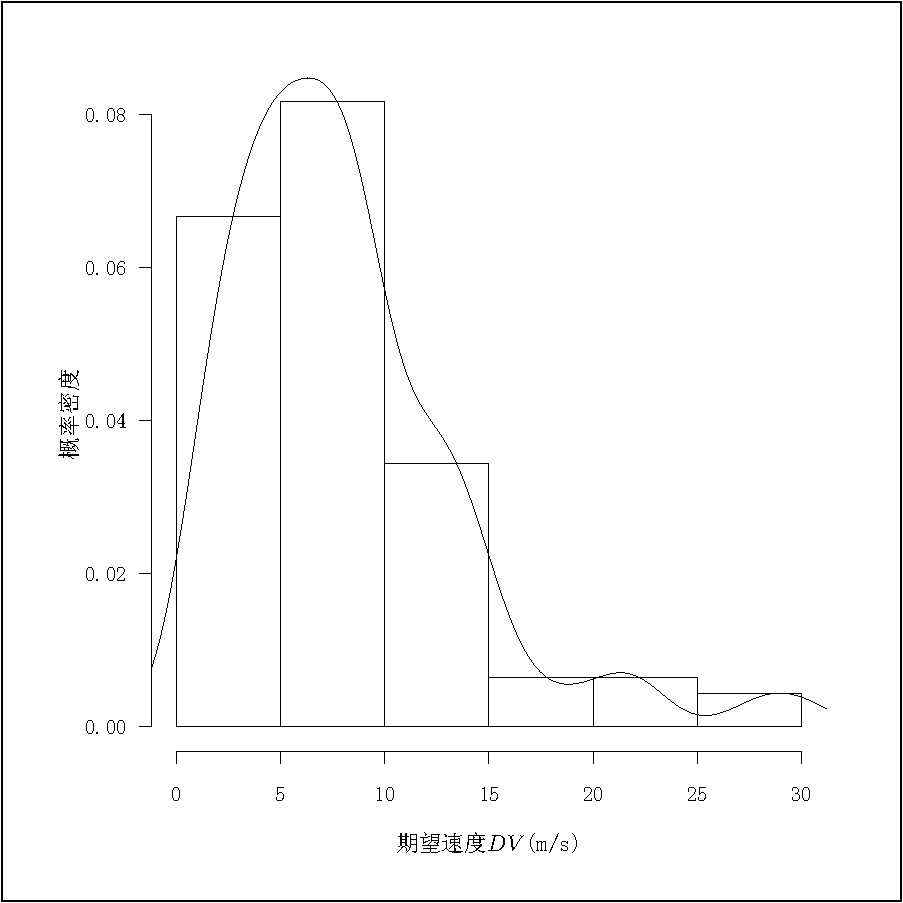
\includegraphics[width=\textwidth]{chapter4-weighted-distr-np1}
\caption{非专业期望速度$DV$分布}
\label{weighted-distr-np1}
\end{minipage}%
\hspace*{0.04\linewidth}
\begin{minipage}[t]{0.48\linewidth}
\centering
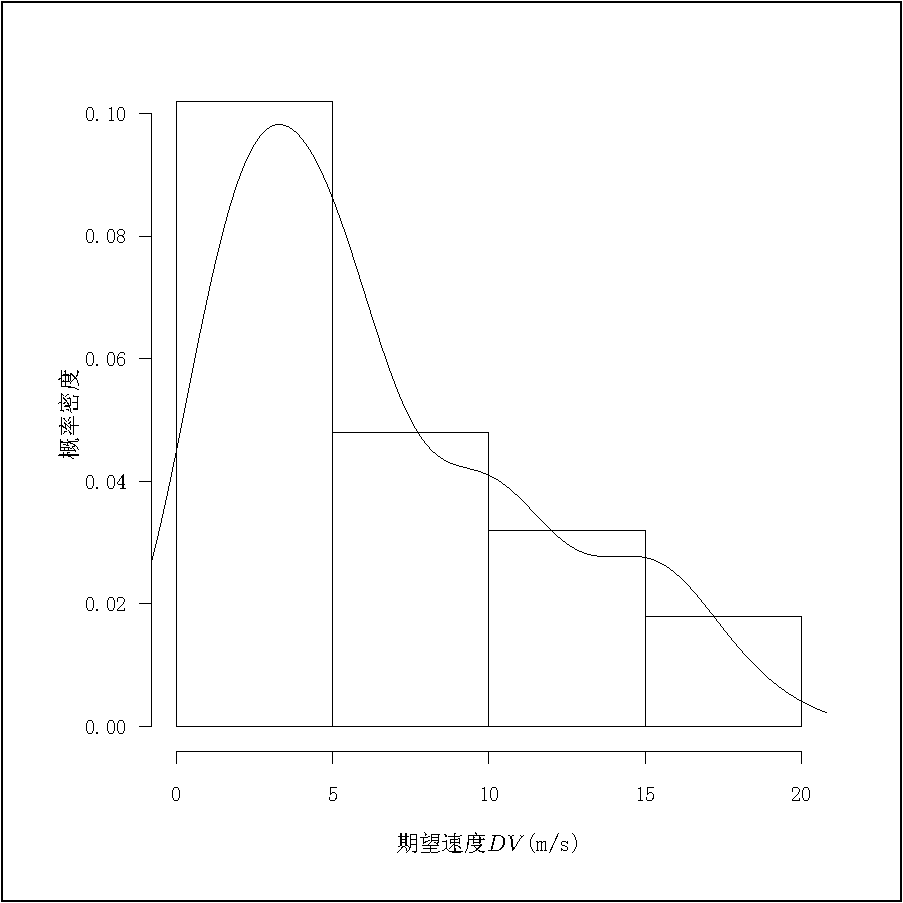
\includegraphics[width=\textwidth]{chapter4-weighted-distr-pp1}
\caption{专业期望速度$DV$分布}
\label{weighted-distr-pp1}
\end{minipage}
\end{figure}

\begin{figure}[htbp]
\begin{minipage}[t]{0.48\linewidth}
\centering
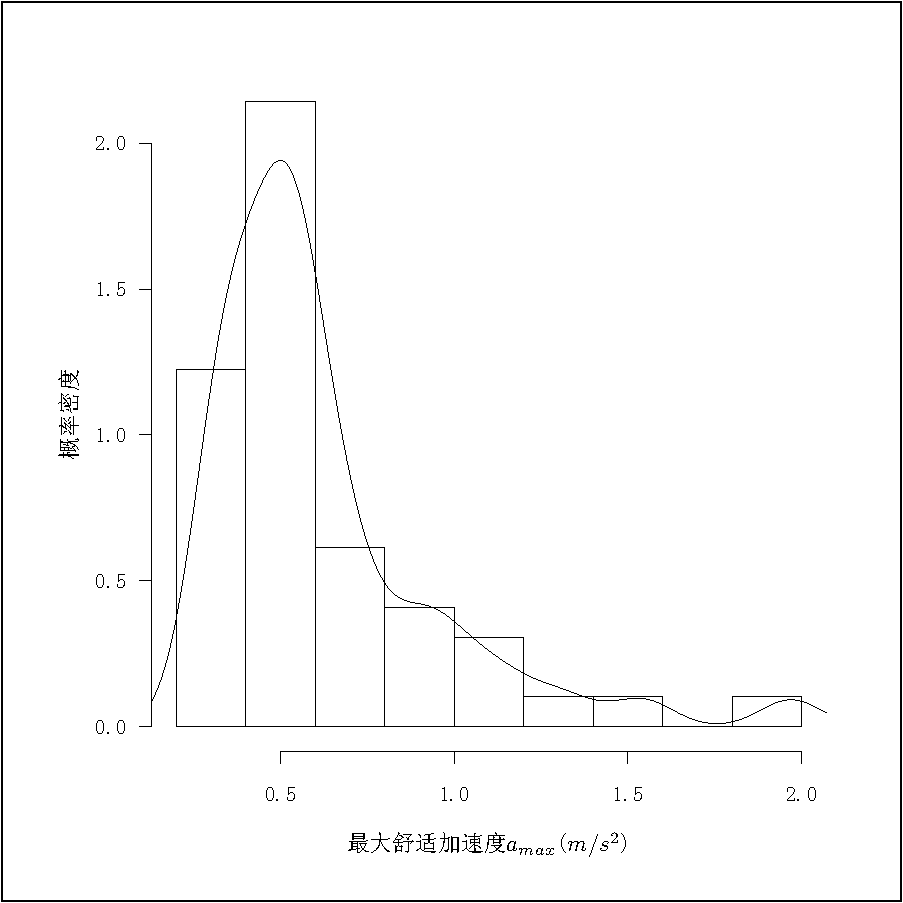
\includegraphics[width=\textwidth]{chapter4-weighted-distr-np2}
\caption{非专业最大舒适加速度$a_{max}$分布}
\label{weighted-distr-np2}
\end{minipage}%
\hspace*{0.04\linewidth}
\begin{minipage}[t]{0.48\linewidth}
\centering
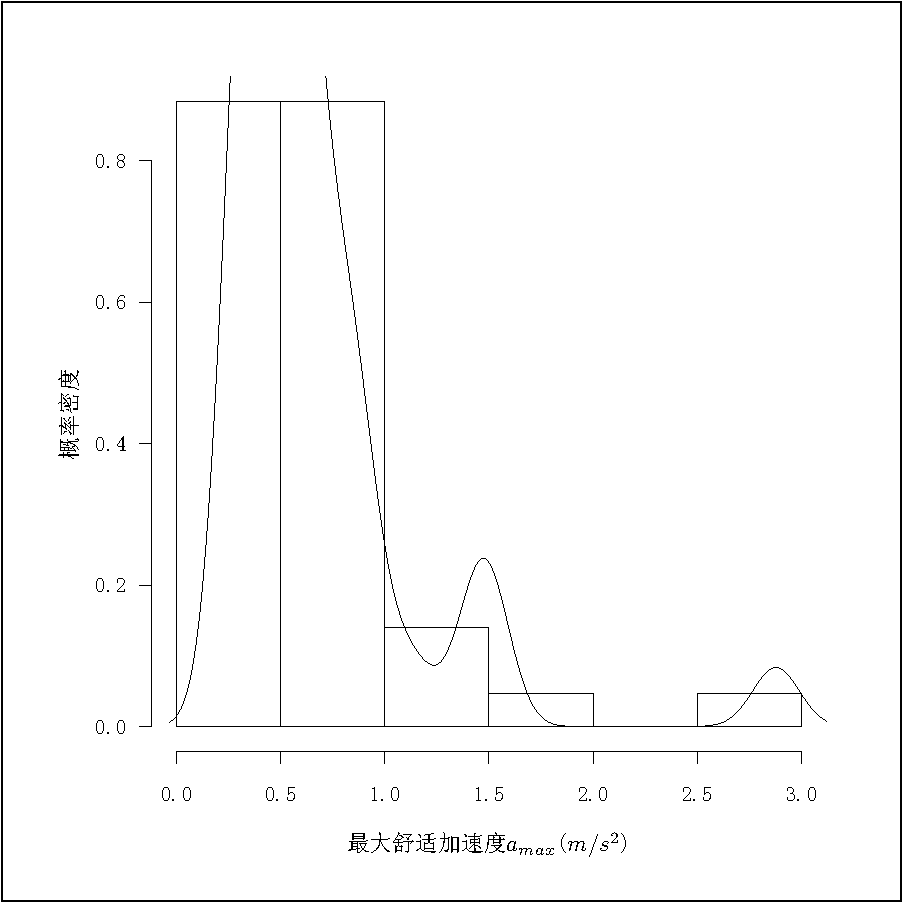
\includegraphics[width=\textwidth]{chapter4-weighted-distr-pp2}
\caption{专业最大舒适加速度$a_{max}$分布}
\label{weighted-distr-pp2}
\end{minipage}
\end{figure}

\begin{figure}[htbp]
\begin{minipage}[t]{0.48\linewidth}
\centering
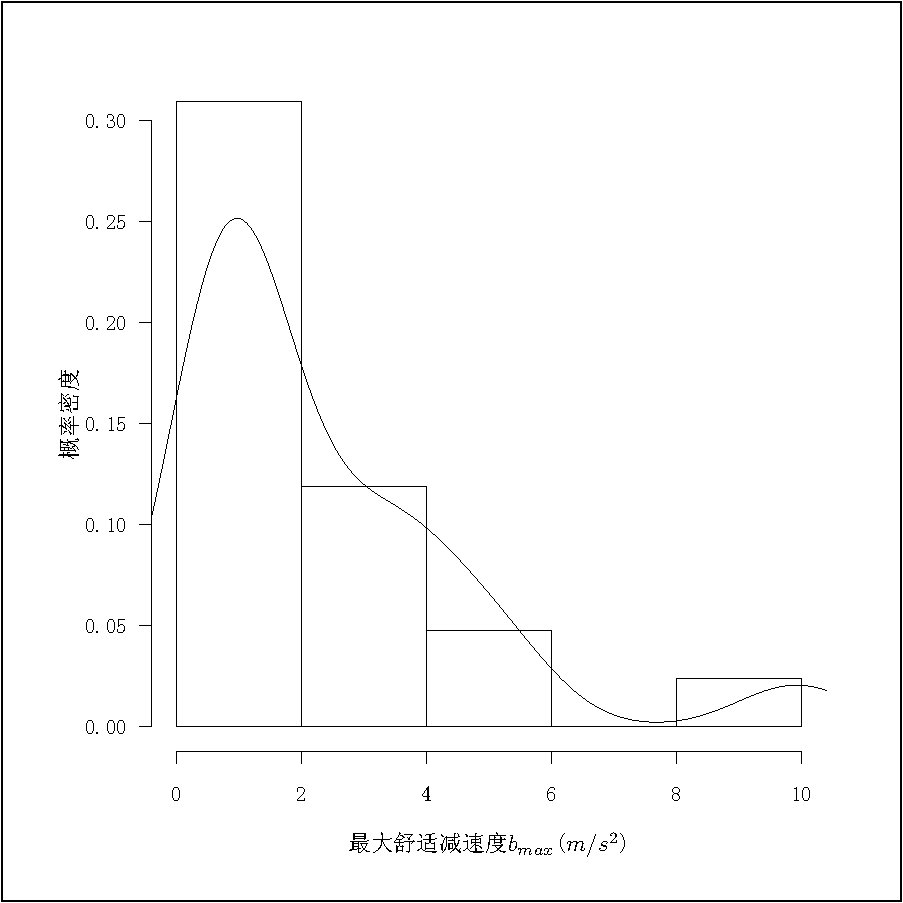
\includegraphics[width=\textwidth]{chapter4-weighted-distr-np3}
\caption{非专业最大舒适减速度$b_{max}$分布}
\label{weighted-distr-np3}
\end{minipage}%
\hspace*{0.04\linewidth}
\begin{minipage}[t]{0.48\linewidth}
\centering
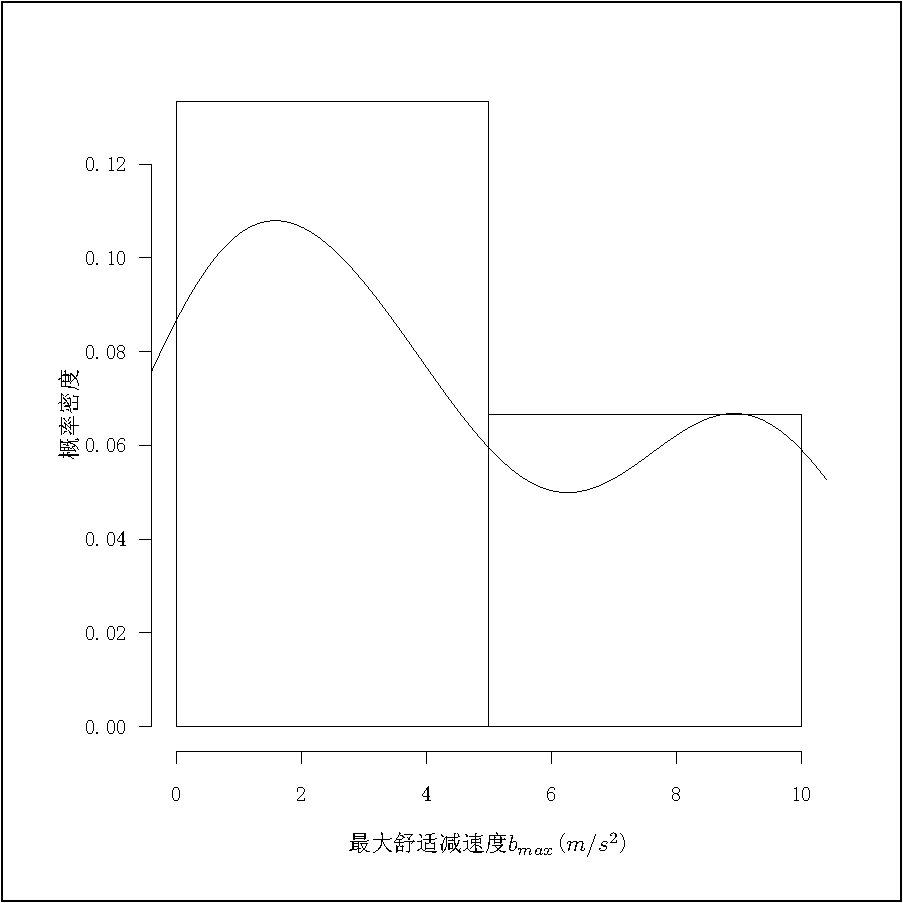
\includegraphics[width=\textwidth]{chapter4-weighted-distr-pp3}
\caption{专业最大舒适减速度$b_{max}$分布}
\label{weighted-distr-pp3}
\end{minipage}
\end{figure}

\begin{figure}[htbp]
\begin{minipage}[t]{0.48\linewidth}
\centering
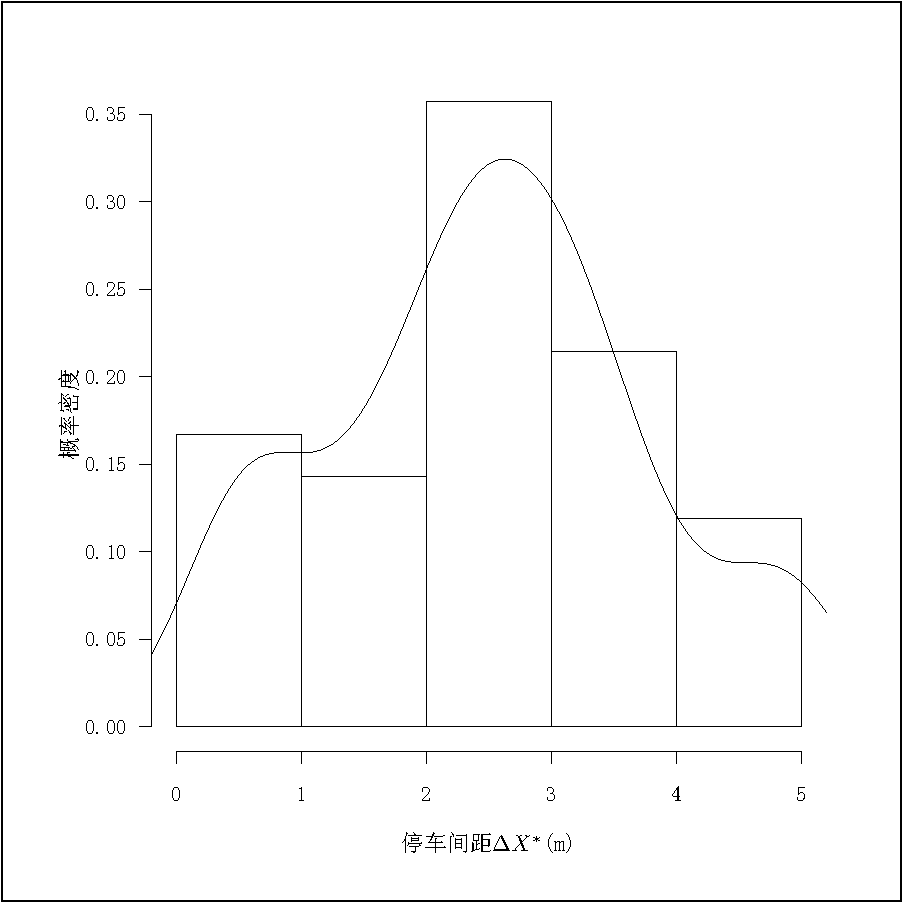
\includegraphics[width=\textwidth]{chapter4-weighted-distr-np4}
\caption{非专业停车间距$\Delta X^*$分布}
\label{weighted-distr-np4}
\end{minipage}%
\hspace*{0.04\linewidth}
\begin{minipage}[t]{0.48\linewidth}
\centering
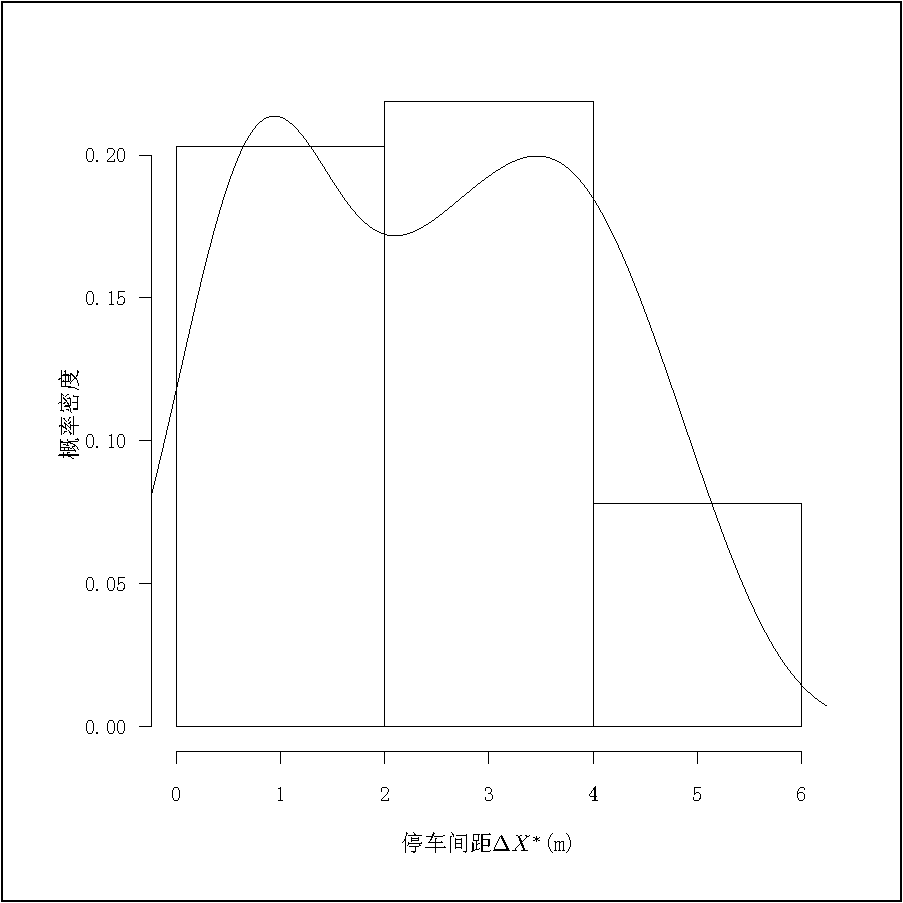
\includegraphics[width=\textwidth]{chapter4-weighted-distr-pp4}
\caption{专业停车间距$\Delta X^*$分布}
\label{weighted-distr-pp4}
\end{minipage}
\end{figure}

\begin{figure}[htbp]
\begin{minipage}[t]{0.48\linewidth}
\centering
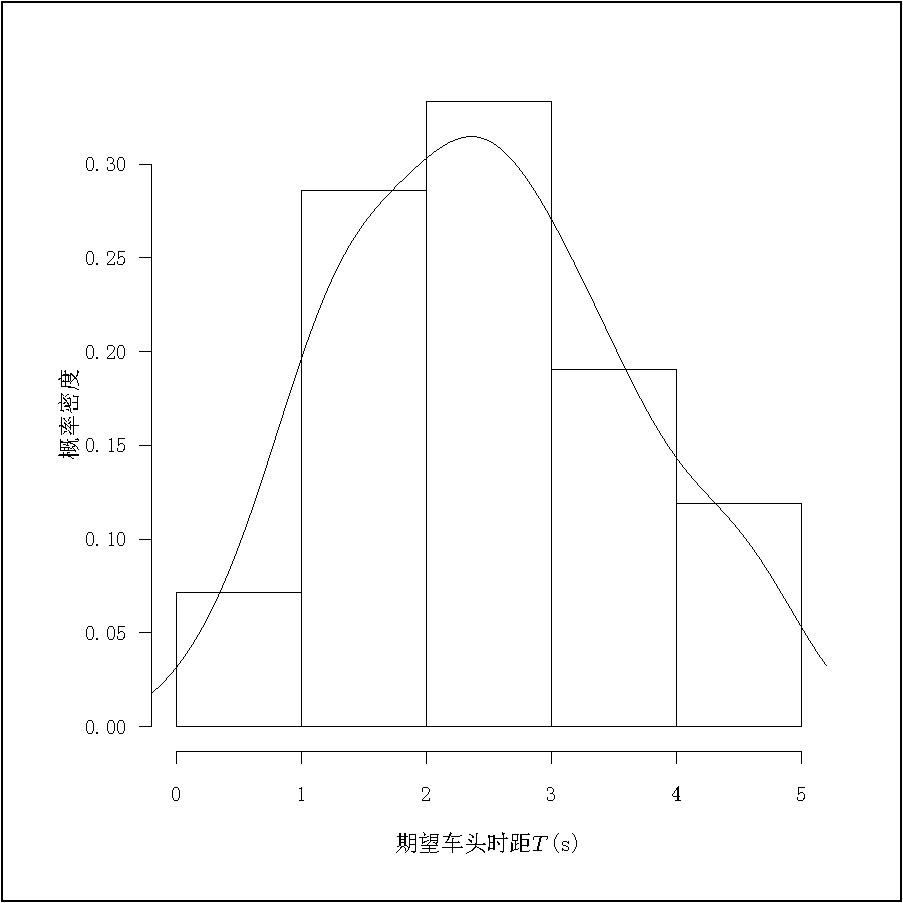
\includegraphics[width=\textwidth]{chapter4-weighted-distr-np5}
\caption{非专业期望车头时距$T$分布}
\label{weighted-distr-np5}
\end{minipage}%
\hspace*{0.04\linewidth}
\begin{minipage}[t]{0.48\linewidth}
\centering
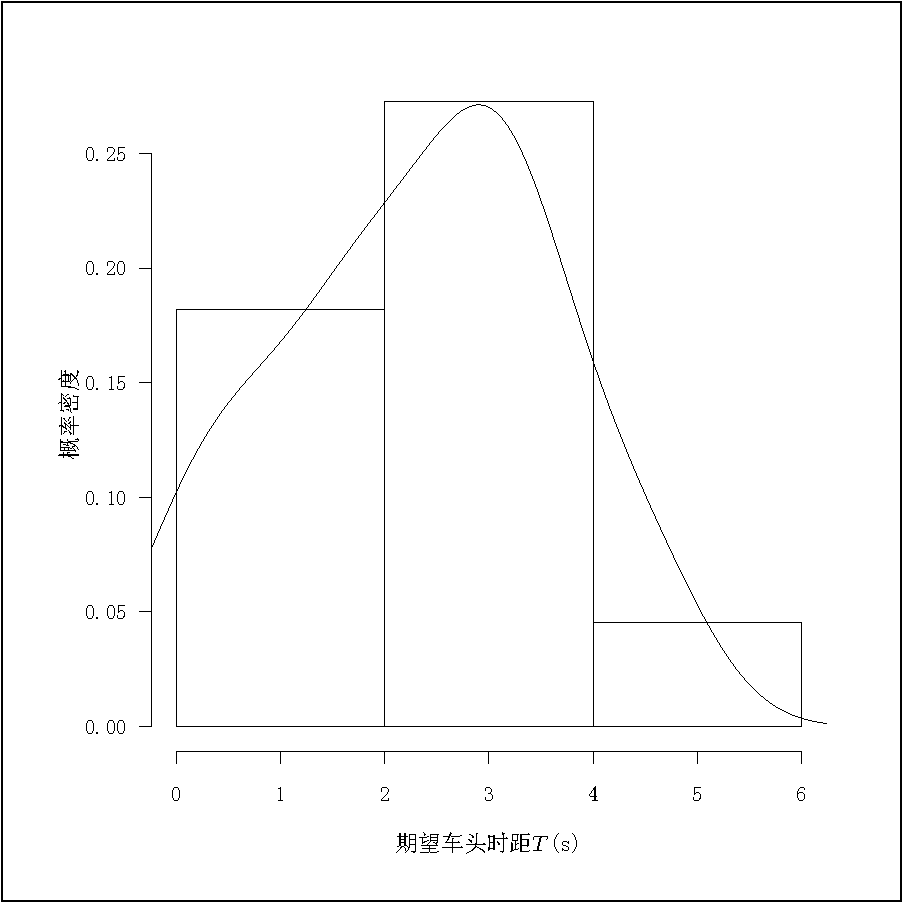
\includegraphics[width=\textwidth]{chapter4-weighted-distr-pp5}
\caption{专业期望车头时距$T$分布}
\label{weighted-distr-pp5}
\end{minipage}
\end{figure}

由图中可以明显看出各参数的样本分布均不符合正态分布,为了得到各参数在总体中的有效估计,并且比较两组驾驶人各参数的异同。本文使用Bootstrap,也称自助法来根据样本数据估计各参数的置信区间。
%bootstrap介绍
%bootstrapping is a computer-based method for assigning measures of accuracy to sample estimates (Efron and Tibshirani 1994). This technique allows estimation of the sample distribution of almost any statistic using only very simple methods (Varian 2005).
Efron(1979)\cite{Efron1979}最早明确提出了Bootstrap方法。Bootstrap方法是非参数统计中一种重要的估计统计量方差进而进行区间估计的统计方法。其核心思想是通过对样本大量(N一般不小于1000)的可重复的重抽样,通过计算重抽样样本的统计量构造Bootstrap分布来近似总体的抽样分布,从而估计样本所属总体的统计量。其渐进有效性对大多数常用分布和统计量已被证明。使用Bootstrap方法主要的优点在于无需对总体的分布进行假设,只需样本中的个体满足独立同分布的条件,便能对总体的统计量(例如均值)进行有效的估计。

对于本文中的数据,相邻轨迹数据的间隔一般都在10s以上。基于驾驶人自身行为具有差异性的假设,可以认为驾驶人在不同时刻的驾驶行为是独立的,那么估计所得各参数值可以认为符合独立同分布的条件。

% an independent and identically distributed population,this can be implemented by constructing a number of resamples of the observed dataset (and of equal size to the observed dataset), each of which is obtained by random sampling with replacement from the original dataset.
%   (1) 采用重抽样技术从原始样本中抽取一定数量(自己给定)的样本,此过程允许重复抽样。   (2) 根据抽出的样本计算给定的统计量T。   (3) 重复上述N次(一般大于1000),得到N个统计量T。   (4) 计算上述N各统计量T的样本方差,得到统计量的方差。

Bootstrap结果中样本均值与总体均值的95\%置信区间估计如\autoref{boot-mean},样本标准差与总体标准差的95\%置信区间估计如\autoref{boot-mean}。Kesting和Treiber(2008)\cite{Kesting2008}的对照结果如\autoref{reference-idm}。可以发现各参数均值均在合理范围内,且非专业组与专业组的参数均值主要在期望速度$DV(m/s)$和最大舒适减速度$b_{max}(m/s^2)$存在差异。

\begin{table}[htbp]
  \centering
  \caption{IDM参数均值估计}
    \begin{tabular}{rrrrr}
    \addlinespace
    \toprule
          & \multicolumn{ 2}{c}{非专业驾驶人} & \multicolumn{ 2}{c}{专业驾驶人} \\
    \midrule
          & 样本均值  & 95\%置信区间 & 样本均值  & 95\%置信区间 \\
    $DV(m/s)$ & 8.09  & (6.978,9.236) & 6.48  & (5.549,7.421) \\
    $a_{max}(m/s^2)$ & 0.63  & (0.531,0.718) & 0.66  & (0.523,0.802) \\
    $b_{max}(m/s^2)$ & 2.33  & (1.362,3.295) & 4.29  & (2.621,5.949) \\
    $\Delta X^*(m)$     & 2.50  & (2.124,2.878) & 2.41  & (1.905,2.931) \\
    $T(s)$     & 2.46  & (2.140,2.783) & 2.34  & (1.810,2.886) \\
    \bottomrule
    \end{tabular}%
  \label{boot-mean}%
\end{table}%

% Table generated by Excel2LaTeX from sheet 'Sheet1'
\begin{table}[htbp]
  \centering
  \caption{IDM参数标准差估计}
    \begin{tabular}{rrrrr}
    \addlinespace
    \toprule
          & \multicolumn{ 2}{c}{非专业驾驶人} & \multicolumn{ 2}{c}{专业驾驶人} \\
    \midrule
          & 样本标准差 & 95\%置信区间 & 样本标准差 & 95\%置信区间 \\
    $DV(m/s)$ & 5.55  & (4.338,6.866) & 4.83  & (4.286,5.440) \\
    $a_{max}(m/s^2)$ & 0.34  & (0.229,0.474) & 0.46  & (0.243,0.724) \\
    $b_{max}(m/s^2)$ & 2.31  & (1.310,3.531) & 3.69  & (3.053,4.593) \\
    $\Delta X^*(m)$    & 1.27  & (1.043,1.523) & 1.50  & (1.305,1.749) \\
    $T(s)$      & 1.12  & (0.936,1.333) & 1.32  & (1.052,1.643) \\
    \bottomrule
    \end{tabular}%
  \label{boot-sd}%
\end{table}%

% Table generated by Excel2LaTeX from sheet 'Sheet1'
\begin{table}[htbp]
  \centering
  \caption{Kesting\cite{Kesting2008}的IDM参数估计}
    \begin{tabular}{rrrr}
    \addlinespace
    \toprule
          & \multicolumn{ 3}{c}{Data Set1} \\
    \midrule
          & $F_{rel}(s)$ & $F_{mix}(s)$ & $F_{abs}(s)$ \\
    误差(\%)     & 24.0  & 20.7  & 20.7  \\
    $DV(m/s)$    & 70.0  & 69.9  & 70.0  \\
    $T(s)$    & 1.07  & 1.12  & 1.03  \\
    $\Delta X^*(m)$    & 2.41  & 2.33  & 2.56  \\
    $a_{max}(m/s^2)$     & 1.00  & 1.23  & 1.40  \\
    $b_{max}(m/s^2)$     & 3.21  & 3.20  & 3.73  \\
    \bottomrule
    \end{tabular}%
  \label{reference-idm}%
\end{table}%
%做均值和SD


对样本的分层Bootstrap,可以获得总体的非专业与专业驾驶人参数均值差的置信区间估计,期望速度$DV(m/s)$和最大舒适减速度$b_{max}(m/s^2)$的Bootstrap分布及正态Q-Q如\autoref{p1-df-qq,p3-df-qq},图中的Bootstrap分布基本上符合正态分布,且样本均值差具有较小的偏差,因此其总体均值差的95\%置信区间是可靠的。置信区间估计结果如\autoref{boot-df},可以看到非专业驾驶人的期望速度大于专业驾驶人,而其最大舒适减速度小于专业驾驶人。

综合以上结果,可以推断在不同的驾驶人之间其期望速度和最大减速度存在差异。期望速度的差异说明驾驶人在大致相同条件下其希望的行驶速度是不同的,这反映了不同驾驶人综合考虑自身需求和对道路交通条件适应的结果。由于样本中非专业组与专业组的年龄存在差异,期望速度的差异可能因为年龄或其他差异而非驾驶经验的差异。而不同驾驶人间最大减速度的差异,反应了驾驶人减速的能力,非专业驾驶人由于驾驶经验较短可能对于潜在的危险情况认识不足,导致其减速能力较低。


% Table generated by Excel2LaTeX from sheet 'Sheet1'
\begin{table}[htbp]
  \centering
  \caption{样本均值差(非专业减去专业)与总体均值差95\%置信区间估计}
    \begin{tabular}{rrr}
    \addlinespace
    \toprule
          & 样本均值差 & 95\%置信区间 \\
    \midrule
    $DV(m/s)$ & 1.60  & (0.072,3.048) \\
    $a_{max}(m/s^2)$ & -0.03  & (-0.204,0.137) \\
    $b_{max}(m/s^2)$ & -1.95  & (-3.774,-0.115) \\
    $\Delta X^*(m)$     & 0.09  & (-0.552,0.751) \\
    $T(s)$     & 0.12  & (-0.519,-0.742) \\
    \bottomrule
    \end{tabular}%
  \label{boot-df}%
\end{table}%

%\begin{figure}[H]
%\begin{center}
%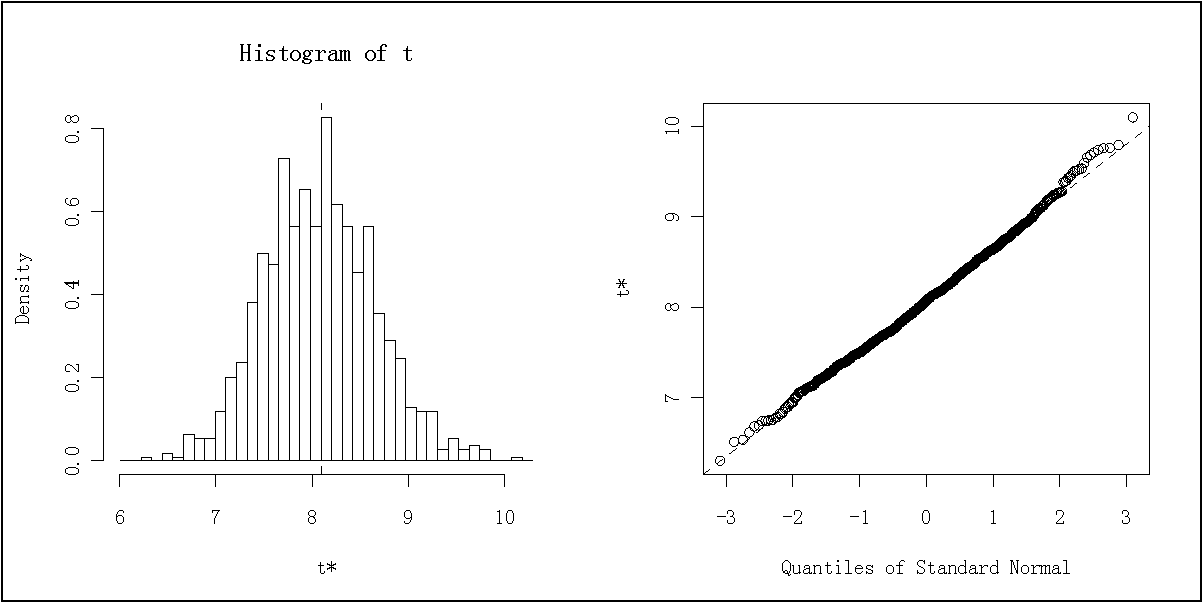
\includegraphics{chapter4-bootstrap-np1-mean.pdf}
%\end{center}
%\caption{非专业驾驶人期望速度$v_{des}$参数Bootstrap分布及正态Q-Q}
%\end{figure}
%
%\begin{figure}[H]
%\begin{center}
%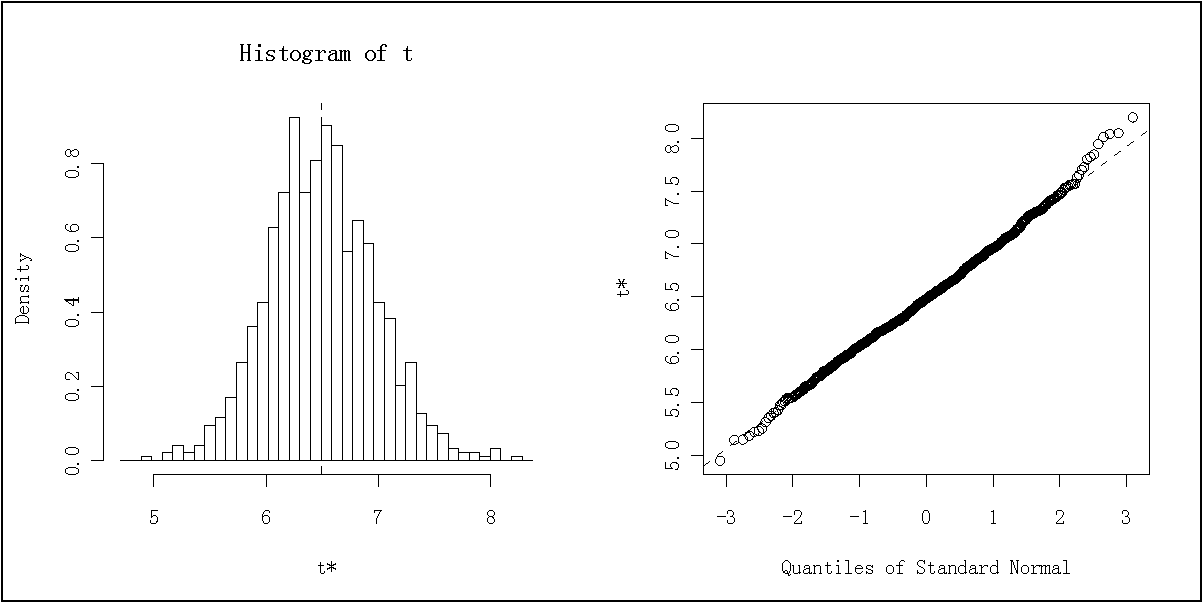
\includegraphics{chapter4-bootstrap-pp1-mean.pdf}
%\end{center}
%\caption{专业驾驶人期望速度$v_{des}$参数Bootstrap分布及正态Q-Q}
%\end{figure}

\begin{figure}[htbp]
\begin{center}
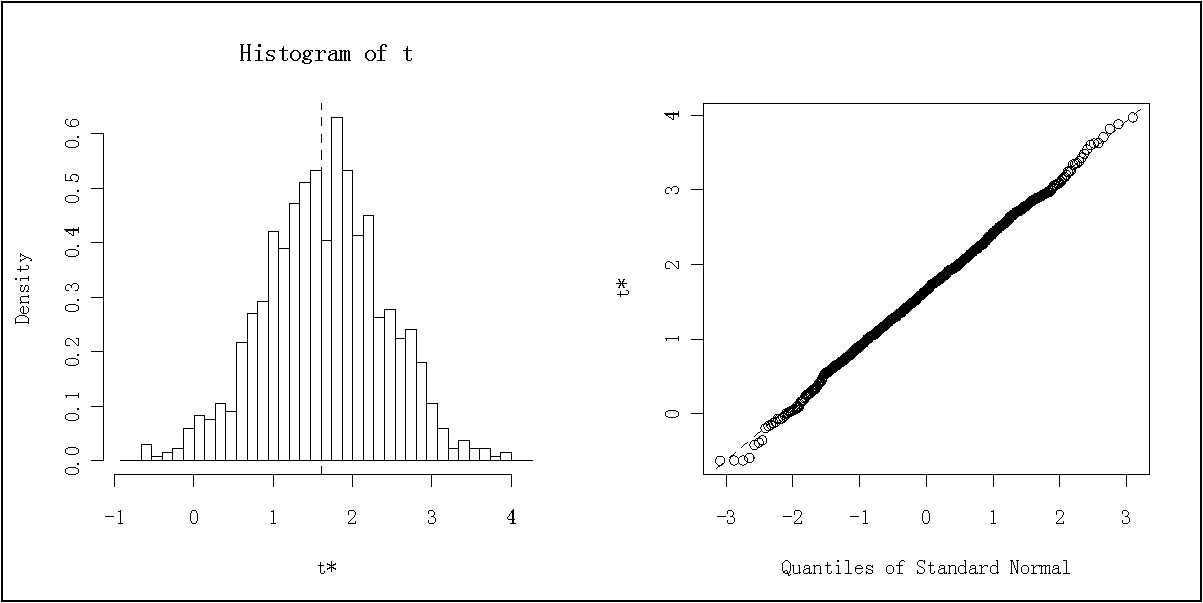
\includegraphics[width=0.6\textwidth]{chapter4-bootstrap-p1df-mean.pdf}
\end{center}
\caption{非专业与专业驾驶人期望速度$v_{des}$参数差值分层Bootstrap分布及正态Q-Q}
\label{p1-df-qq}
\end{figure}





%\begin{figure}[H]
%\begin{center}
%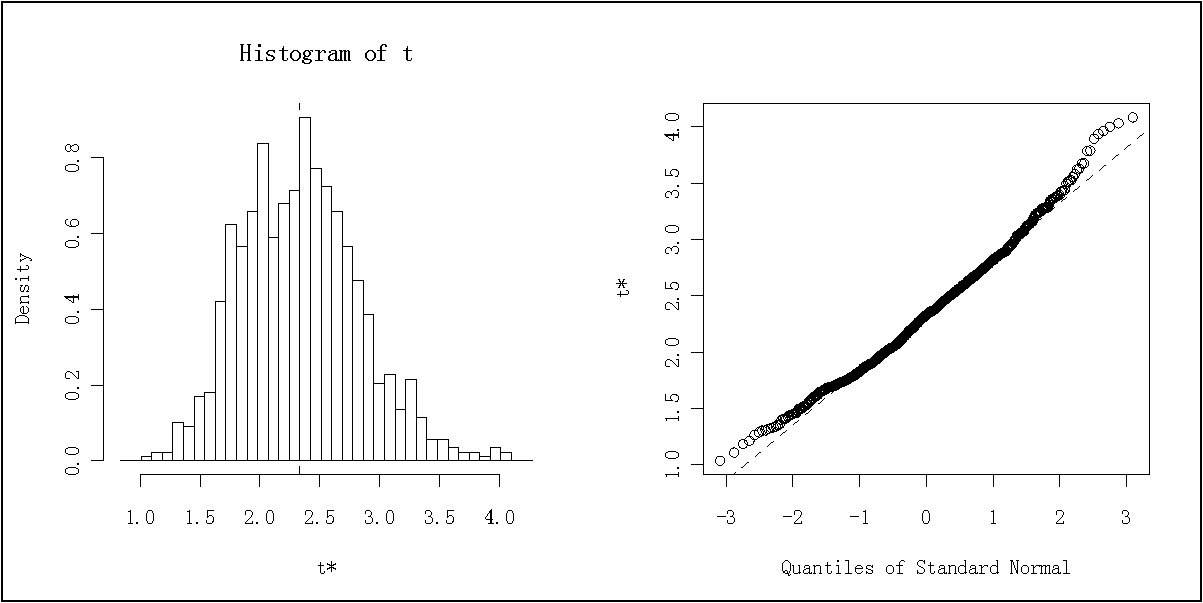
\includegraphics{chapter4-bootstrap-np3-mean.pdf}
%\end{center}
%\caption{非专业驾驶人最大舒适减速度$b_{max}$参数Bootstrap分布及正态Q-Q}
%\end{figure}
%
%\begin{figure}[H]
%\begin{center}
%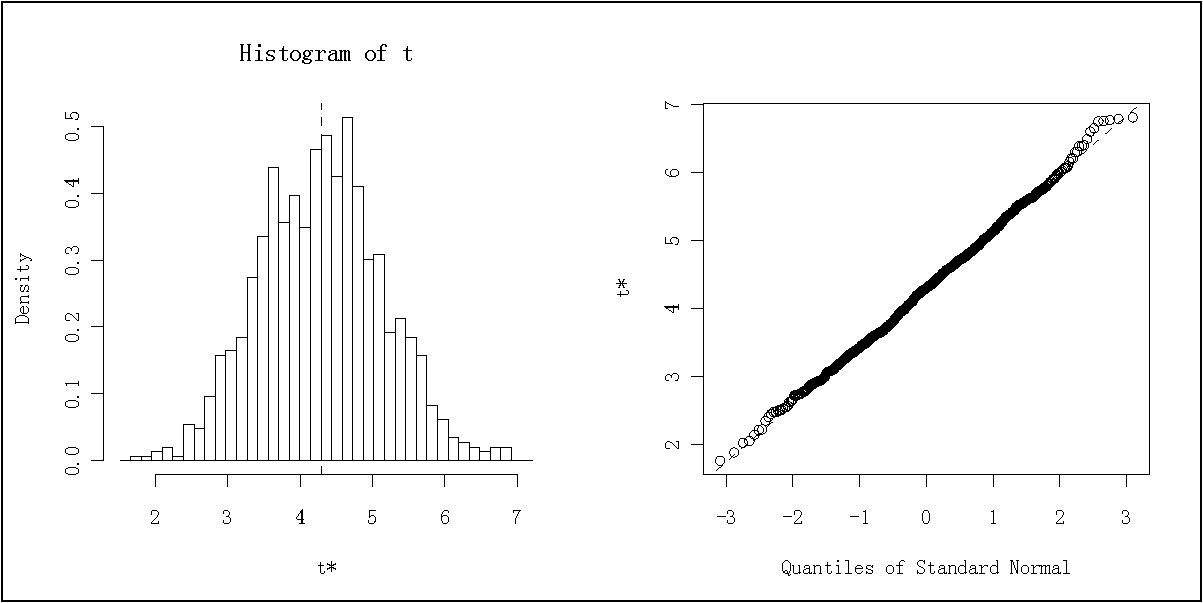
\includegraphics{chapter4-bootstrap-pp3-mean.pdf}
%\end{center}
%\caption{专业驾驶人最大舒适减速度$b_{max}$参数Bootstrap分布及正态Q-Q}
%\end{figure}

\begin{figure}[htbp]
\begin{center}
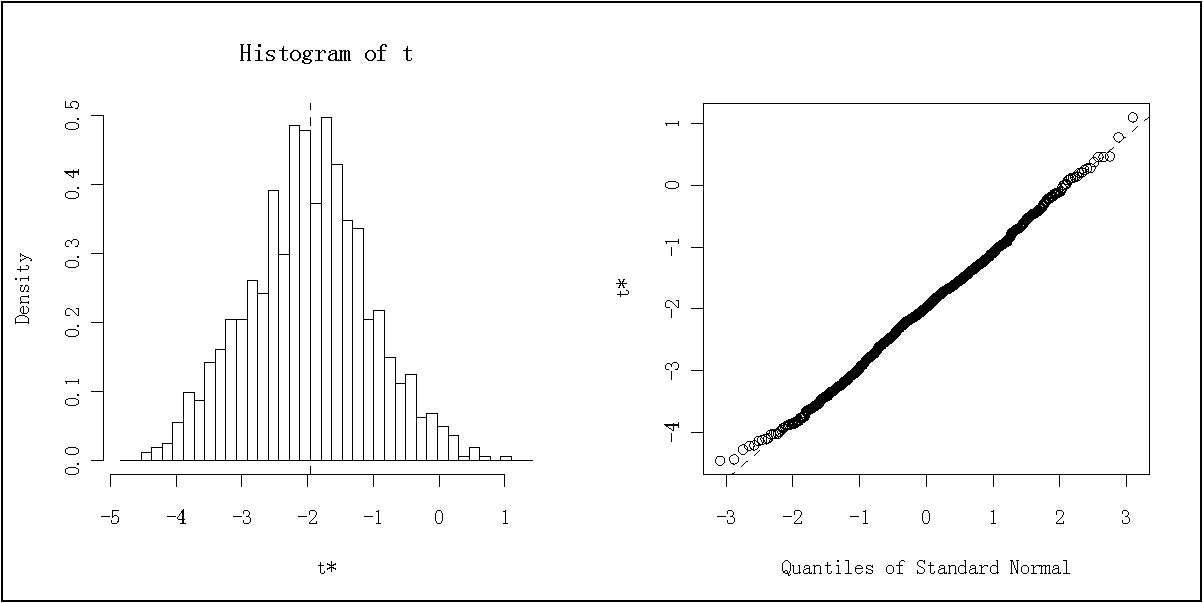
\includegraphics[width=0.6\textwidth]{chapter4-bootstrap-p3df-mean.pdf}
\end{center}
\caption{非专业与专业驾驶人最大舒适减速度$b_{max}$参数差值分层Bootstrap分布及正态Q-Q}
\label{p3-df-qq}
\end{figure}








%
%free us from the tedious assumptions
%bca confidence interval

%permutation test
%requirements



\section{本章小结}
本章通过对所采集数据进行处理和分析,研究了驾驶人行为特性的异同,发现非专业组和专业组驾驶人在自由行驶与跟驰的临界点,期望速度和最大减速度方面存在差异,为下一章研究驾驶人行为特性对交通流影响提供了依据。

\chapter{驾驶人行为特性对交通流影响分析}


\section{驾驶行为建模}
\section{路段交通流仿真}
\section{交通流影响分析}
\chapter{结论与展望}

本文在假设专业与非专业驾驶人驾驶行为存在差异的基础上,通过自行设计的实验,收集了大量的数据,分析了专业驾驶人与非专业驾驶人驾驶行为特性的异同,并通过微观模拟仿真的方法研究了驾驶人行为特性对交通流的可能影响。

\section{主要成果和结论}
\subsection{研究方法}
设计并应用车载激光测距仪、车载GPS卫星定位系统、摄像机同步实时监测实验车辆的驾驶人行为特性关键指标,获取大量真实有效的实验数据。获得了跟车实验的大概的有效数据获取率为40\%,为进一步研究提供了数据量的参考。

给出了使用跟驰模型参数标定和Bootstrap方法估计驾驶人参数的方法框架,以及通过模拟分析驾驶行为特性对交通流影响的思路。

\subsection{关于驾驶人行为特性的发现}
研究表明,驾驶人所采取的减速度与TTC倒数呈现较为明显的线性关系,驾驶人在加减速方面存在不对称性。

专业和非专业两组驾驶人的跟驰与自由流临界点特性方面存在差异。通过参数标定表明,驾驶人在期望速度和最大减速度方面存在差异。


\subsection{驾驶人行为特性对交通流的影响}

最小通行能力似乎取决于所有驾驶人中的最低期望车速。期望车速对基本图上的速度流量曲线的形状产生影响,且主要在自由流阶段。

高期望速度导致TTC倒数绝对值的时间密度增加,低期望车速驾驶人混入少于高期望车速驾驶人时,TTC倒数绝对值的时间密度变化较大。


最大减速度的增加,导致密度流量图上较难达到通行能力的区域,且在J线以上较为不稳定的同步流状态。

最大减速的增加导致总模拟时间有增加的趋势。少量高最大减速度的驾驶人的混入时,即使模拟时间较大增加,并且模拟时间的变化范围较大。

对于具有不同最大减速度的驾驶人,似乎存在最佳的混合比例使得TTC倒数绝对值的时间密度最小。

混合作用影响下随着B型驾驶人(代表专业驾驶人)的增加,TTC倒数的绝对值的最大值在相同流量下有增加的趋势,表明相同流量下专业驾驶人的增加导致交通流偏向不安全的方向。

期望速度与最大减速度共同影响时,最大减速度影响的效应占了主要成分,表明相比期望速度最大减速度是影响交通流关键的因素。


\section{研究所存在的问题}

由于本文收集的驾驶人数据量,就驾驶人个数而言还较小,这导致样本的代表性存在不足,例如样本中女性驾驶人较少。

样本中专业组和非专业组驾驶人除了在驾驶经验方面存在差异之外在平均年龄上也存在差异,因此驾驶行为的差异可能不是由于驾驶经验的差异导致的。

本文中由于实验条件的限制未对变道行为进行更多讨论。

%由于不存在完全模拟现实的模型存在,模拟所得出的结果也没有完备的理论支撑,因此结果应当审慎地对待。



\section{研究展望}

可以考虑改进研究设备,例如增加激光测距仪的光线条数来获取变道行为的数据。要获得更确定性的结论,应当对更多涉及范围更广的驾驶人进行更长时间的研究。

可以考虑使用其他模型或者通过实际测试的方法来验证驾驶人行为特性对交通流的影响。

研究表明驾驶人的减速度与交通流关系密切,这为辅助驾驶系统的研究提供了更多的动机和条件。

%更多的考虑交通流的安全性的评价

%(1)	设计了一种新的研究驾驶人行为特性的实验方法
%在对驾驶人行为特性定义与分类的基础上,应用车载激光测距仪、车载GPS卫星定位系统、摄像机同步实时监测实验车辆的驾驶人行为特性关键指标,利用调查问卷了解必要的驾驶人心智特性。本实验能够克服传统调查实验中的各种不足与缺点,能够获取大量真实有效的实验数据,在国内是首次采用车载激光测距仪、GPS和摄像机相结合的方式同步实时监测实验车辆。
%(2)	研究了城市道路上驾驶人行为特性的规律
%针对驾驶人行为特性的关键指标,研究了在单向两车道与单向三车道城市道路上,驾驶人在速度、车头间距和车头时距方面的规律。分析了速度、车头间距和车头时距的分布及其统计特征值,通过对车头间距和车头时距统计值的进行回归分析,得到专业驾驶人和非专业驾驶人的车头间距与速度之间关系的拟合函数和车头时距与速度之间关系的拟合函数。
%(3)	建立的驾驶人行为特性对城市路段通行能力的修正模型
%利用专业驾驶人与非专业驾驶人车头间距与速度之间关系的拟合函数和车头时距与速度之间关系的拟合函数,分别得到基于车头间距与车头时距的路段通行能力模型,并给出了两种路段通行能力模型在各速度下,混合交通流的通行能力驾驶人修正系数推荐值。为了消除误差,取两者的平均值作为最后推荐值,得到基于驾驶人行为特性的城市路段通行能力模型,并给出不同道路条件各速度下,驾驶人混合交通流的通行能力驾驶人修正系数推荐值。
%(4)	对论文提出的通行能力模型与通行能力修正系数进行仿真
%通过仿真程序对论文提出的城市道路路段通行能力模型和推荐的通行能力修正系数进行模拟检验,可视、直观的表现出驾驶人混合交通流对城市道路路段通行能力的影响。


\end{Main} % 结束正文

\begin{Thanks}
感谢……
\end{Thanks}

\bibliography{seuthesis}
%\bibliographystyle{seuthesis}

\begin{Appendix}
  \chapter{第一个附录}% latex table generated in R 2.12.0 by xtable 1.5-6 package
% Thu Mar 03 12:36:06 2011
\begin{table}[ht]
\begin{center}
\begin{tabular}{rrlrlrrr}
  \hline
 & ID & sex & age & license & certified & mileage & pro \\ 
  \hline
1 & 1.00 & 女 & 25.00 & C1 & 0.50 & 0.00 & 0.00 \\ 
  2 & 2.00 & 男 & 23.00 & C1 & 1.00 & 0.50 & 0.00 \\ 
  3 & 3.00 & 男 & 26.00 & C1 & 4.00 & 2.00 & 0.00 \\ 
  4 & 4.00 & 女 & 24.00 & C1 & 2.50 & NA & 0.00 \\ 
  5 & 5.00 & 男 & 24.00 & C1 & 4.00 & 0.60 & 0.00 \\ 
  6 & 6.00 & 男 & 26.00 & C1 & 5.00 & 1.00 & 0.00 \\ 
  7 & 7.00 & 男 & 26.00 & C1 & 4.00 & 0.50 & 0.00 \\ 
  8 & 8.00 & 男 & 23.00 & C1 & 4.00 & 0.20 & 0.00 \\ 
  9 & 9.00 & 男 & 24.00 & C1 & 5.00 & 1.50 & 0.00 \\ 
  10 & 10.00 & 男 & 24.00 & C1 & 3.00 & 1.00 & 0.00 \\ 
  11 & 11.00 & 男 & 28.00 & C1 & 1.00 & 0.50 & 0.00 \\ 
  12 & 12.00 & 男 & 25.00 & C1 & 1.00 & 0.80 & 0.00 \\ 
  13 & 13.00 & 女 & 24.00 & C1 & 3.00 & 2.50 & 0.00 \\ 
  14 & 14.00 & 男 & 24.00 & C1 & 2.00 & 2.00 & 0.00 \\ 
  15 & 15.00 & 男 & 29.00 & C1 & 5.00 & NA & 0.00 \\ 
  16 & 16.00 & 男 & 25.00 & C1 & 4.00 & 15.00 & 0.00 \\ 
  17 & 17.00 & 男 & 39.00 & NA & 3.00 & 24.00 & 1.00 \\ 
  18 & 18.00 & 男 & 44.00 & A & 11.00 & 90.00 & 1.00 \\ 
  19 & 19.00 & 男 & 37.00 & A & 10.00 & NA & 1.00 \\ 
  20 & 20.00 & 男 & 33.00 & B & 16.00 & 30.00 & 1.00 \\ 
  21 & 21.00 & 男 & 43.00 & B & 6.00 & 60.00 & 1.00 \\ 
  22 & 22.00 & 男 & 45.00 & A & 23.00 & 200.00 & 1.00 \\ 
  23 & 23.00 & 男 & NA & A & 10.00 & 50.00 & 1.00 \\ 
  24 & 24.00 & 男 & 50.00 & NA & 14.00 & 15.00 & 1.00 \\ 
  25 & 25.00 & 男 & 53.00 & NA & 18.00 & 60.00 & 1.00 \\ 
  26 & 26.00 & 男 & 47.00 & A & 15.00 & 76.00 & 1.00 \\ 
   \hline
\end{tabular}
\label{basic_table}
\end{center}
\end{table}

  \chapter{第二个附录}
  ……
\end{Appendix}

\newpage
\printindex % 索引

\begin{Resume}
作者简介
\end{Resume}
\backcover
\end{document}
